\documentclass{report}
\usepackage[utf8]{inputenc}
\usepackage{amssymb}
\usepackage{amsthm}
\usepackage{nicematrix}
\usepackage{subcaption}
\usepackage{pdfpages}
\usepackage{algpseudocode}
\DeclareMathOperator*{\argmin}{arg\,min}

\usepackage{listings}
\lstset { %
    language=C++,
    backgroundcolor=\color{white}, % set backgroundcolor
    numbers=none,
    frame=shadowbox,
    basicstyle=\footnotesize,% basic font setting
}

\NiceMatrixOptions{cell-space-top-limit = 4pt}
\NiceMatrixOptions{cell-space-bottom-limit = 4pt}

\usepackage{bm}
\usepackage{appendix}

\newtheorem{definition}{Definition}
\newtheorem{proposition}{Proposition}
\newtheorem*{remark}{Remark}

\usepackage{amsmath}
\usepackage{graphicx}
\usepackage{xcolor}
\usepackage{tcolorbox}
\tcbuselibrary{theorems}
\newtcbtheorem
  []% init options
  {tcb-def}% name
  {Definition}% title
  {%
    colback=green!5,
    colframe=green!35!black,
    fonttitle=\bfseries,
  }% options
  {def}% prefix
\newtcbtheorem
  []% init options
  {tcb-prop}% name
  {Proposition}% title
  {%
    colback=blue!5,
    colframe=blue!80!black,
    fonttitle=\bfseries,
  }% options
  {prop}% prefix

\usepackage{natbib}
\usepackage[figurename=Fig.,tablename=Tab.,labelfont={bf}]{caption}
\usepackage{listings}
\usepackage{tikz}
\usetikzlibrary{positioning, decorations.markings, arrows, intersections}
\bibliographystyle{apalike}
\setcitestyle{authoryear,open={(},close={)}} %Citation-related commands
\usepackage[linkbordercolor=green]{hyperref}
\usepackage{geometry}
\geometry{a4paper,scale=0.8}

\definecolor{codegreen}{rgb}{0,0.6,0}
\definecolor{codegray}{rgb}{0.5,0.5,0.5}
\definecolor{codepurple}{rgb}{0.58,0,0.82}
\definecolor{backcolour}{rgb}{0.95,0.95,0.92}

\lstdefinestyle{mystyle}{
    backgroundcolor=\color{backcolour},   
    commentstyle=\color{codegreen},
    keywordstyle=\color{magenta},
    numberstyle=\tiny\color{codegray},
    stringstyle=\color{codepurple},
    basicstyle=\ttfamily\footnotesize,
    breakatwhitespace=false,         
    breaklines=true,                 
    captionpos=b,                    
    keepspaces=true,                 
    numbers=left,                    
    numbersep=5pt,                  
    showspaces=false,                
    showstringspaces=false,
    showtabs=false,                  
    tabsize=2
}

\lstset{style=mystyle}

\newcommand{\mathcolorbox}[2]{\colorbox{#1}{$\displaystyle #2$}}
\newcommand{\note}[1]{{\footnotesize \textcolor{blue}{[\textbf{#1}]}}}

\title{\textbf{Asymptotic-preserving Plasma Model in 3D}}
\author{Tianwei Yu}
\date{\today}


\begin{document}

\begin{titlepage}
\noindent \includegraphics[]{ETHlogo.pdf}

\centering
\vspace*{7cm}

\textbf{\LARGE Asymptotic-Preserving Plasma Model in 3D}

\vspace{3cm}
\large

Master thesis

\vspace{0.25cm}

\textbf{Tianwei Yu}

\vspace{0.25cm}

\today

\vspace{7cm}

Supervisor: Prof. Dr. Ralf Hiptmair

\vspace{0.25cm}

Department of Mathematics, ETH Z\"{u}rich




\end{titlepage}

\chapter*{Abstract}
Plasma physics involves complex phenomena characterized by multiple scales, for example, the propagation of electromagnetic fields, the interaction between charged particles and electromagnetic fields, and the drift of fluids. To numerically simulate plasmas, discretization schemes that can automatically adapt to the scale of interest and remain stable regardless of the system scales are desirable. In this thesis, we discuss asymptotic-preserving (AP) schemes for the Euler-Maxwell system parametrized by the dimensionless Debye length $\lambda$ in a 3D setting for multi-species plasma modeling. The key capability of the AP scheme is the uniform performance, in the sense of stability and convergence, for a series of problems that are parametrized by arbitrary $\lambda$ and constitute a singular perturbation as $\lambda \rightarrow 0$. As the first part of the thesis, the AP property, still being a vague concept throughout literature, is clarified by two aspects: asymptotic-stability and asymptotic-consistency, which respectively refer to the unconditional stability on the asymptotic parameter and the convergence of the limit scheme to the limit model. Two propositions discussing some sufficient conditions for general AP schemes are presented, hopefully providing deeper insights into the AP property and some guidance for devising AP schemes. In the sequel, we reproduce the results in \cite{degond_2012}, based on which we extend the 1D two-fluid discrete Euler-Maxwell model to a more general model in a 3D setting that involves multiple species, friction terms, and possibly other source terms. The 3D discrete model for the Euler-Maxwell system is implemented based on the frameworks of Finite Volume Method (FVM) and Finite Integration Technique (FIT) for the Euler system and the Maxwell system respectively. Details about the procedure of time-stepping and the assembly of the linear system due to implicitness are provided. An essential aspect lies in the choice of right boundary conditions that are compatible with both non-limit and limit models. The discrete model is tested on a case that is adapted from \cite{fuchs_2021} due to the difficulty arising from the insulating solid domain. As verification, the scheme is checked on the subsystems and is compared with the corresponding 1D discrete model. The numerical results on the fully-coupled system with $\lambda$ ranging in $[0,1]$ manifest a continuous transition from the non-neutral model ($\lambda = \mathcal{O}(1)$) to the quasi-neutral model ($\lambda = 0$), which, as well as the convergence of the solutions over time, implies that the scheme is AP.                             

\chapter*{Acknowledgements}
First, I would like to extend my deepest gratitude to my supervisor Prof. Ralf Hiptmair. His proposal for this thesis combines fluid dynamics, a topic that I am familiar with, and electromagnetism, a completely new world for me. With reasonable amounts of theoretical and implementation work, I had much fun in the process of freely exploring the knowledge and accomplishing the task step by step. His constant and insightful input was always inspiring at the moment when I was lost. In a word, it was a pleasant, adventurous, and memorable journey.

My appreciation also goes to Dr. Roman Fuchs, who gave me a lot of guidance on familiarizing myself with the topic and the underlying C++ code. I would also like to acknowledge the help of my colleague Langwen Huang in the configuration of the running environment on the cluster, which potentially saved me considerable time.

Meanwhile, I would like to thank my girlfriend, friends, and flatmates for their company and support during the thesis work as well as my Master's life. I wish them all a bright future.  

In the end, I would like to express my special gratitude to my parents for their financial support and emotional care. They are always my strongest back no matter what setbacks I encounter.



\tableofcontents
\chapter{Introduction}
\section{Plasma}
Often described as the fourth state of matter, plasma is an ionized gas phase substance that consists of positively-charged \emph{ions}, negatively-charged \emph{electrons} and neutrally-charged atoms. Although plasmas seem to be intangible in our daily life, most of the material in the universe is in the plasma state \citep{gurnett2005}. They are largely associated with various astrophysical phenomena like sunspots, solar flares, planetary radiation belts. Regarding terrestrial plasmas, they can be found or exploited in many situations, for instance, lightning, gas-discharge lamps, controlled thermonuclear fusion.     

A plasma is classically defined as \emph{a quasi-neutral gas of charged particles showing collective behavior} \citep{chen_1994}. The \emph{collective} behavior arises due to the long-range nature of $1/r$ Coulumb potential \citep{gibbon2020}. Besides, the dynamics of plasma particles are largely determined by an internally-driven electromagnetic field, in the sense that the charges generate an electric field, and carry an electric current that induces a magnetic field. In contrast, a gas in a neutral state is largely characterized by inter-particle collision. The second key feature, \emph{quasi-neutrality}, refers to the tendency to keep the overall charges neutral in the scale of the Debye length $\lambda_D$, which is an important plasma parameter and will be elucidated in the later section. 

In classical plasma theory, three criteria must be satisfied to distinguish plasmas from ionized gases \citep{chen2016}. First, the quasi-neutrality requires that the Debye length $\lambda_D$ is much smaller than the system scale $L$. Second, to make the quasi-neutrality a statistically valid concept, the number $N_D$ of particles in a ``Debye sphere ", namely $N_D := n4/3\pi\lambda_D^3$ with $n$ being the number density of particles, must be large enough. The third criterion states the dominance of the electromagnetic forces over the hydrodynamics forces in driving the motions of particles.

\subsection{Fluid model}
To describe the dynamics of plasmas, a natural and extremely precise way is to treat it as a collection of particles and to monitor the positions and velocities of each particle, namely \emph{N-body dynamics}. It has been proven powerful in analytically describing effects relevant to plasmas \citep{escande2015}.  However, a typical plasma density might be $10^{18}$ particles per $m^3$ \citep{chen2016}, which is way far from affordable for today's computers if one attempts to numerically simulate it. Therefore, relatively crude models are necessary for plasma simulations. The \emph{kinetic model} is another successful tool to describe plasmas. It compiles the state of a collection of particles in the form of probabilistic distributions of velocity and usually consists of the Vlasov-Maxwell equations with velocity distribution functions as variables. See \cite{chaudhary2018} for details on the kinetic description of plasmas.  

An even simpler model, \emph{fluid model}, described by the Euler-Maxwell equations, can be derived by taking the moments of the Vlasov-Maxwell equations supplemented with some closure assumption. Specifically, we take the velocity distribution to be $Maxwellian$, by which the distribution can be characterized by its moments. In this way, the fluid model describes the evolution of the moments, e.g. number density, drift velocity, pressure, rather than the distribution. Such a treatment reduces the complexity of the system at the cost of some information. This bridging between the fluid model and the kinetic model applies reasonably for ordinary hydrodynamics where the Maxwellian velocity distribution results from frequent collisions. It seems problematic for a plasma since generally, the collision rate is very low in a plasma due to its dilute nature. However, the experimental work of \cite{langmuir1925} demonstrates the surprising validity of the Maxwellian assumption for plasmas. This phenomenon is known as \emph{Langmuir paradox} which remains unsolved. Readers are referred to \cite[][p. 63]{chen2016} for some discussions. It is worth noting that the fluid model suffices for the majority of plasma phenomena, but certain situations exist where neither the fluid model is applicable, nor is the kinetic theory.

In the fluid model of plasma, each species of particles is equipped with a full set of fluid equations into which the Lorentz force and other plasma effects are incorporated. Maxwell's equations govern how an electromagnetic field is generated by the charged fluids, their motions, and changes of the fields. For such a coupled system, various assumptions are usually made to reduce complexity according to specific scenarios. In the simplest case, one considers a fully-ionized plasma and treats the ions, which are about $10^4$ times heavier than electrons, to be immobilized. Such simplification makes sense when phenomena at the scale of electron motions are of particular interest, and thus leads to so-called \emph{one-fluid} model\footnote{In this report, we think of ions, electrons, and neutral atoms as `fluid', and each `fluid' is described by a set of fluid equations. Also, `species' and `fluid' are synonymous here. Notice that in some literature they have different meanings.} in the sense that only one set of fluid equations is sufficient. To study more realistic situations, motions of multiple species of particles ought to be simulated. Furthermore, other effects like viscosity, ionization, recombination, and collisions could play important roles in many applications.         

\subsection{Quasi-neutrality} \label{sec:quasi-neutrality}
Let's imagine such a situation: in a neutral\footnote{It means the net charge vanishes everywhere.} plasma with temperature $T_0$ and electron number density $n_0$, the electrons contained in cube volume $d^3$ are, due to thermal motions, separated from ions. The non-zero charge thus gives rise to an induced electric field, and the energy required for this movement is of magnitude $n_0e^2d^2 / \varepsilon_0$ for a single particle. In the absence of external forces, this energy must come only at the expense of the thermal energy \citep{frank_1972}, which is of magnitude $k_BT_0$. Only when the energy required for the displacement is less than the thermal energy can this local unbalance of charges happen. By balancing these two energy magnitudes we get the length scale

\begin{equation*}
    d \sim \left(\frac{\varepsilon_0k_BT_0}{e^2n_0}\right)^{1/2} =: \lambda_D
\end{equation*}
which is termed \emph{Debye length}\footnote{The Debye length is usually defined for electrons. In fact, one can define different Debye lengths for other species.}. The Debye length is a fundamental property of nearly all plasmas of interest \citep{gibbon2020}. Being a crucial plasma parameter, it is a characteristic length scale over which the perturbation of electric charges is screened due to random thermal motions. With a small $\lambda_D$, the mismatch of positive and negative charges would be limited to a small area. Hence the plasma is approximately \emph{neutral}, namely canceling out in net charges, over a relatively large spatial scale. Such phenomenon of effectively shielding the electrostatic field within a distance of the order $\lambda_D$ is called \emph{Debye shielding}.

Now comes the illustration of \emph{quasi-neutrality}, which is a common property of plasmas. Consider $L_0$ as the characteristic length scale of the system, upon which the dimensionless Debye length $\lambda$ is readily defined as
\begin{equation*}
    \lambda := \frac{\lambda_D}{L_0}.
\end{equation*}
When $\lambda_D$ is much smaller than $L_0$, any local charge unbalance is shielded out within distance of the order $L_0$. The quasi-neutrality refers to such a situation that the plasma is neutral enough such that one can take $\rho \approx 0$, but not so neutral that all the interesting electromagnetic forces vanish \citep{chen2016}. In other words, the quasi-neutrality does not render the plasma a neutral gas such that it has no interaction with the electromagnetic field. 

From a mathematical viewpoint, the quasi-neutrality assumption causes the degeneracy of Gauss's law for the electric field to the quasi-neutral condition $\rho = 0$. Despite the vanishing electric charge $\rho$, the electric field is \emph{not} divergence-free. Such degeneracy of the system poses challenges when one has to deal with the non-neutral and quasi-neutral models---two systems of different mathematical properties---at the same time.

\section{Asymptotic-preserving schemes}
 Many important partial differential equations (PDEs) systems involve asymptotic parameters (denoted by $\lambda$ from now on), which might take value from $\lambda = \mathcal{O}(1)$ to $\lambda \ll 1$ at different regimes of the targeting problem, e.g. the relaxation of collision term (or Knudsen number \textbf{Kn}) in Boltzmann equations, Mach number \textbf{Ma} in the Navier-Stokes (N-S) equations, and the Debye length $\lambda_D$ in the Euler-Maxwell system. These parameters have close connections with the characteristic scale of the system, e.g. wave speed and relaxation time. As the asymptotic parameter $\lambda$ approaches zero, the limit solution (if exists) is described by a set of PDEs of a different type from the non-limit one. A \emph{singular perturbation} problem hence arises (See \cite{mark_1995} for related theories). For instance, the Boltzmann equation tends to the compressible N-S equations as \textbf{Kn} $\rightarrow 0$; the compressible N-S equations approach the incompressible case as \textbf{Ma} $\rightarrow 0$, and the fluid pressure switches its hyperbolic character to the elliptic one. To give an intuition about the singular perturbation, consider a toy model
 \begin{equation} \label{equ:toy-model}
     \lambda u' + u = 0, u:[0,\infty]\rightarrow\mathbb{R},
 \end{equation}
 which is a first-order ordinary differential equation (ODE). Let $\lambda$ go to zero, the (pointwise) limit solution satisfies 
 \begin{equation*}
     u = 0,
 \end{equation*}
 which is no longer a first-order ODE.
 
 Following \cite{jin_2010}, we refer to the original system ($\lambda = \mathcal{O}(1)$) as \emph{microscopic} model while the limiting system ($\lambda \rightarrow 0$) as \emph{macroscopic} model, denoting them by $P^\lambda$ and $P^0$ respectively. If either the macroscopic or the microscopic model is uniformly valid in the whole domain, one can devise schemes accordingly. In fluid dynamics, for example, different solvers are tailored for compressible and incompressible flows. Applying schemes for $\lambda = \mathcal{O}(1)$ to the problem with $\lambda \ll 1$ would be problematic because schemes for $P^\lambda$ are usually subject to CFL-like conditions dependent on $\lambda$. For instance, \textbf{Ma} is inversely proportional to the sound speed; Debye length is inversely proportional to the wave speed. Under-resolving these small scales usually lead to instability. Therefore, $\lambda \ll 1$ would pose very strict restriction on time-step size, leading to prohibitive computational cost. Look back to the toy model (\ref{equ:toy-model}). A reasonable scheme for $\lambda = \mathcal{O}(1)$ is the explicit Euler
 \begin{equation*}
     \lambda\frac{u^{n+1}-u^{n}}{\delta} + u^n = 0.
 \end{equation*}
Yet obviously if the time-step size $\delta$ is fixed, it does not apply to arbitrarily small $\lambda$ due to the stability condition $\delta < 2\lambda$.  
 
 The standard strategy to handle problem $P^\lambda$ with $\lambda \ll 1$ is to solve $P^0$ instead of $P^\lambda$ under the assumption that $P^0$ is a good approximation of $P^\lambda$. For instance, the fluid limit of the Boltzmann equation removes the restrictive stability condition that is dependent on a small relaxation length; the incompressible N-S equations eliminate the need to resolve the sound speed whereas it is necessary in the compressible case. However, challenges occur when sub-domains with $\lambda = \mathcal{O}(1)$ and $\lambda \ll 1$ coexists in the computational domain. To mention some examples, the reentry problem of space shuttles involves both rarefied and dense gases; the plume of a convergence-divergence nozzle experiences \textbf{Kn} from small to very large value \citep{jenny2015}; the plasma sheath near the wall area violates the quasi-neutral assumption in contrast to the quasi-neutral bulk area. To handle such hybrid problems, the classical approach is to split the domain and apply schemes accordingly. However, the criterion for domain splitting is not straightforward and quite empirical. In addition, the projection of solutions from one model to another in the transitional area adds to complexity \citep{jin_2010, degond_2011}. In other words, the non-uniformity of numerical schemes on microscopic and macroscopic models poses a great challenge in handling problems in a transitive regime.
 
 This dilemma spurs tremendous interests in developing schemes that work \emph{uniformly} well for $\lambda \in [0,1]$ with fixed spatial/time step. Such a scheme is expected to produce satisfactory results without resolving the smallest scale and provide a more elegant and unified solution to problems in a transitive regime. At this point, we introduce the concept of \emph{asymptotic-preserving} (AP) schemes. We resort to the celebrated commuting diagram Fig. \ref{fig:illustration_ap} in \cite{jin_1999} which sketches the property that an AP scheme should possess. As is defined above, $P^\lambda$ and $P^0$ stand for the (solutions of) microscopic and macroscopic models respectively. We introduce the discrete model $P^\lambda_h$ based on some AP scheme, whose solution depends on both the asymptotic parameter $\lambda$ and the spatial (or temporal) step size $h$. We stress that each limit in Fig. \ref{fig:illustration_ap} is attained by letting one parameter go to zero while fixing the other. As a basic requirement, the discrete microscopic model $P^\lambda_h$ should at least converge to its analytic solution $P^\lambda$ as $h\rightarrow0$. The AP property additionally allows the convergence of $P^\lambda_h$ to the limit discrete model $P^0_h$ as $\lambda\rightarrow0$. To accomplish this aim, the stability restriction on $h$ must be independent of $\lambda$. We refer to such property as \emph{asymptotic stability}, following \cite{degond_2011}. Furthermore, the discrete macroscopic model $P^0_h$ must again converge to the macroscopic model $P^0$ as $h\rightarrow0$. Such property is termed \emph{asymptotic consistency}. In other words, a discrete model (scheme) $P^\lambda_h$ is AP if it satisfies the commuting diagram Fig.\ref{fig:illustration_ap}. To make it intuitive, AP schemes preserve the asymptotic limits from the microscopic to the macroscopic models, \emph{at the discrete level} \citep{jin_2010}.
 
  \begin{figure}
     \centering
     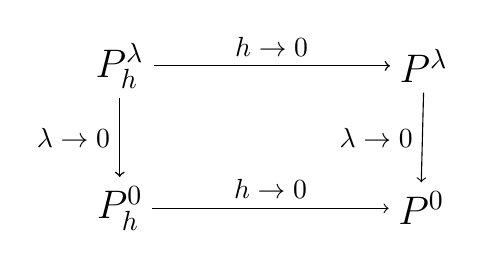
\begin{tikzpicture}
     \node (nw) {\Large $P^\lambda_h$};
     \node (ne) [right=3cm of nw]{\Large $P^\lambda$};
     \node (sw) [below=of nw]{\Large $P^0_h$};
     \node (se) [right=3cm of sw]{\Large $P^0$};
     \draw[->] (nw.east)  -- node [above,midway] {$h\rightarrow0$} (ne.west) ;
     \draw[->] (nw.east)  --  (ne.west) ;
     \draw[->] (nw.south) -- node [left,midway] {$\lambda\rightarrow0$} (sw.north);
     \draw[->] (nw.south) -- node {} (sw.north);
     \draw[->] (sw.east)  -- node [above,midway] {$h\rightarrow0$}(se.west);
     \draw[->] (ne.south) -- node [left,midway] {$\lambda\rightarrow0$} (se.north);
     \end{tikzpicture}
     \caption{Illustration of AP schemes}
     \label{fig:illustration_ap}
 \end{figure}
 
 We present the definition in a formal way: 
 \begin{definition} \label{def:ap}
 Consider the microscopic model $P^\lambda$ depending on an asymptotic parameter $\lambda$, and assume the macroscopic model $P^0$ exists as the asymptotic limit as $\lambda \rightarrow 0$. The discrete model $P^\lambda_h$, depending both on $\lambda$ and $h$, is \emph{asymptotic-preserving} if
 \begin{itemize}
     \item $P^\lambda_h$ converges to $P^\lambda$ as $h\rightarrow0$ with stability conditions independent of $\lambda$ \emph{(asymptotic stability)};
     \item the asymptotic limit model $P^0_h$ is consistent with $P^0$ \emph{(asymptotic consistency)}.
 \end{itemize}
 \end{definition}
 Looking back again to the model (\ref{equ:toy-model}), one can easily verify that the implicit Euler
 \begin{equation*}
     \lambda\frac{u^{n+1}-u^{n}}{\delta} + u^{n+1} = 0
 \end{equation*}
 is AP. 
 
 Extra properties are also desirable in some cases. In kinetic models with relaxations \citep{jin_2010}, for example, the scheme that can drive \emph{any} initial data into the local equilibrium \emph{in one step} is referred to as \emph{strongly AP}. Instead, if the local equilibrium is reached after long enough, it is referred to as \emph{relaxed AP}. If the initial data is well-prepared and the equilibrium remains for good, it is \emph{weakly AP}. Yet in this thesis, we are only concerned about the essential part of AP property that is specified in Definition \ref{def:ap}.
 
 Note that the existence of a macroscopic model $P^0$ as the asymptotic limit of microscopic model $P^\lambda$ is presumed. Rigorous proofs of some cases are available, for instance, in \cite{friedman_1968} for general linear PDEs, \cite{klainerman_1981} for the incompressible limit of the Euler equations, \cite{chen_1994, natalini_1996} for conservation laws with stiff relaxation term; \cite{remi_2014} for quasi-neutrality limit in the Euler-Maxwell system. This topic is beyond the scope of this thesis and we just take for granted the existence of such limit models. 
 
 The concept of AP schemes can be traced back to \cite{jin_1995} in which the authors approximate a conservation law by a hyperbolic system with relaxation, and manage to construct a scheme that is stable for an arbitrarily small relaxation parameter. The term ``asymptotic-preserving" was formally introduced in \cite{jin_1999} for handling the diffusive regime of kinetic models. This concept stemmed from and remains very active in kinetic models with stiff relaxations, see \cite{jin_2010} and the references therein. Nonetheless, considerable effort has been put into developing AP schemes for many other problems that admit asymptotic behavior. For instance, in fluid dynamics, the so-called \emph{all-speed} schemes are advantageous when dealing with both compressible and incompressible regimes simultaneously. \cite{degond_2007, haack_2010} devise all-speed schemes for the isentropic Euler equations through fast-slow decomposition of velocity fields. Concerning plasma physics, a number of papers are available dealing with the quasi-neutral limit of the Euler-Poisson (or Euler-Maxwell) system \citep{crispel_2005, degond_2008, degond_2011, degond_2012} and Vlasov-Poisson (or Vlasov-Maxwell) system \citep{degond_2017, degond2017b, zhu_2017}. Besides, \cite{caflisch_1997, berthon2011} concern AP schemes for generic hyperbolic systems with relaxation source terms. For a comprehensive review on AP schemes, readers are referred to \cite{jin_2010} for kinetic and hyperbolic equations, and \cite{degond_2017} for multiscale plasma simulations. 
 
 To devise an AP scheme, one mostly has to consider which terms need to be evaluated implicitly to meet the requirements of the AP property \citep{degond_2011} since stronger stability is usually achieved through implicit treatment in time discretization. We want to stress that unconditionally-stable (with respect to $\lambda$) schemes are not necessarily AP \citep{degond_2011,caflisch_1997}\footnote{It means the asymptotic stability does not necessarily lead to asymptotic consistency as is defined in definition \ref{def:ap}.}. Furthermore, a fully-implicit scheme is very likely to possess AP property, but the computational difficulties arising from solving massive linear or possibly nonlinear equations is potentially a huge cost. As is summarized by \cite{degond_2017}, AP schemes aim to bridge several sets of equations describing the system in different regimes, rather than to alleviate the stability constraints of the numerical methods. In this sense, a fully-implicit scheme is likely to be overkill. We want to achieve the AP property without incurring too much extra cost, which necessitates a smart construction.    
 
 A general methodology for devising AP schemes is suggested by \cite{degond_2012, degond_2017}. They summarize it into two steps. The first step is a ``reformulation" step, where an equivalent form $R^\lambda$ of $P^\lambda$ is to be found such that the $R^\lambda$ explicitly appears as a perturbation of $P^0$. Afterward, one discretizes $P^\lambda$ by a scheme $P^\lambda_h$ with a certain amount of implicitness in such a way that the reformulation procedure can be performed at the discrete level, and leads to a reformulated discrete model $R^\lambda_h$ that is consistent to $R^\lambda$. However, this procedure is somehow heuristic, and its applicability to other perturbation problems remains questionable. It is also infeasible to rigorously prove the AP property for a given scheme, which is largely owing to the fuzzy notations of ``convergence" of numerical schemes. Even the linearized stability, as a necessary condition, is difficult to analyze in a multi-dimensional framework. Therefore, for the time being, we can state the AP property and devise the AP scheme merely in a heuristic way, and mostly has to resort to numerical experiments for verification. 
 
 To summarize, the advantage of AP schemes over classical ones is twofold: for problems involving different regimes, the macroscopic regime ($\lambda \ll 1$) does not suffer from the strict stability requirement whereas the microscopic regime ($\lambda \sim \mathcal{O}(1)$) can be resolved as usual; the scale of interest, namely the resolution that we desire, is free to choose regardless of the value of the asymptotic parameter that represents the scale of the system.  


\chapter{Discussion on Asymptotic-preserving Property}

On portraying the AP property through the commuting diagram Fig. \ref{fig:illustration_ap} and Definition \ref{def:ap}, we convey the principle of how an AP scheme is supposed to behave. Yet these illustrations are somehow given in general terms and lack precise statements. Another concern lies in the potential entanglement between the two requirements of AP schemes, namely asymptotic stability and asymptotic consistency Since these two statements are very strong, decomposing them into weaker ones is likely to help identify essential components to yield AP property. Due to the shortage of theoretical analysis on AP schemes, we humbly make some attempts here.

In this chapter, the AP property, as well as the related arguments, are rephrased in a relatively rigorous way. Specifically, we want to explore the connection of the four asymptotic relations depicted in the commuting diagram Fig. \ref{fig:illustration_ap}, relying on which we try to present an argument about a set of sufficient conditions that lead to an AP scheme. 

Based on the formulation the commuting diagram Fig. \ref{fig:illustration_ap}, we rephrase the AP property by a uniform convergence statement: a discrete model $P^\lambda_h$ is AP if and only if
\begin{equation} \label{arg:ap}
    \exists C, k > 0,\ \ \  \|P^\lambda_h - P^\lambda\| \leq Ch^k,\ \ \ \forall \lambda \in [0,1]  
\end{equation}
where $\|\cdot\|$ represents some suitable norm.
We repeat the definitions: the asymptotic parameter $\lambda$; the discretization parameter $h$, e.g., time step size and cell size; the (solution of) discrete model $P^\lambda_h$; the (solution of)  continuous model $P^\lambda$. This amounts to stating a scheme that converges to the analytical solution uniformly well for arbitrary $\lambda$ and especially for the macroscopic model $P^0$, which is nothing but the philosophy of AP schemes. 

Next, we present an argument that relates the convergence relationships in the commuting diagram with the above uniform convergence statement.
\begin{proposition} \label{prop:1}
Assume $P^0_h$ is well-defined. If the following conditions are satisfied
\begin{itemize}
    \item[$(*)$] $P^\lambda_h \xrightarrow[]{h\rightarrow0}P^\lambda$ in the sense that $\exists \alpha, \Tilde{\alpha}, C_1$ being constant independent of $h, \lambda$ such that
    \begin{equation*}
        \|P^\lambda_h - P^\lambda\| \leq C_1\frac{h^\alpha}{\lambda^{\Tilde{\alpha}}},\ \ \ \forall \lambda \in (0,1],
    \end{equation*}
    \item[$(**)$] $P^\lambda_h \xrightarrow[]{\lambda\rightarrow0} P^0_h$ in the sense that $\exists \beta, C_2$ being constant independent of $h, \lambda$ such that
    \begin{equation*}
        \|P^\lambda_h - P^0_h\| \leq C_2\lambda^\beta,\ \ \ \forall h > 0,
    \end{equation*}
    \item[$(\$)$] $P^\lambda \xrightarrow[]{\lambda\rightarrow0}P^0$ in the sense that $\exists C_3, \gamma$ being constant independent of $h, \lambda$ such that
    \begin{equation*}
        \| P^\lambda - P^0\| \leq C_3\lambda^\gamma, \ \ \ \forall \lambda \in [0,1],
    \end{equation*}
\end{itemize}
Then we have $P^\lambda_h \xrightarrow[]{h\rightarrow0} P^\lambda$ uniformly on $\lambda$, namely argument (\ref{arg:ap}).
\end{proposition}
\begin{proof}
Let $\epsilon$ be a constant satisfying $\alpha - \epsilon > 0$. For any $\lambda \in [0,1]$, we have the following two situations.

If $\lambda^{\Tilde{\alpha}} < h^{\alpha - \epsilon}$, we pick $\Tilde{\lambda} = h^\frac{\alpha - \epsilon}{\Tilde{\alpha}}$, and we have
\begin{align*}
    \|P^\lambda_h - P^\lambda\| &\leq \|P^\lambda_h - P^{\Tilde{\lambda}}_h\| + \|P^{\Tilde{\lambda}}_h - P^{\Tilde{\lambda}}\| + \|P^{\Tilde{\lambda}} - P^\lambda\| \\
    & \leq C_2(\lambda^\beta + \Tilde{\lambda}^\beta) + C_1\frac{h^\alpha}{{\Tilde{\lambda}}^{\Tilde{\alpha}}} + C_3(\Tilde{\lambda}^\gamma + \lambda^\gamma) \\
    & \leq 2C_2h^{\frac{\alpha - \epsilon}{\Tilde{\alpha}}\beta} + C_1h^\epsilon + 2C_3 h^{\frac{\alpha - \epsilon}{\Tilde{\alpha}}\gamma} \\
    & \leq 5\text{max}\{C_1,C_2,C_3\}h^{\text{min}\{\frac{\alpha - \epsilon}{\Tilde{\alpha}}\beta, \epsilon, \frac{\alpha - \epsilon}{\Tilde{\alpha}}\gamma\}}.
\end{align*}
The triangle inequality is applied to the first and second inequalities. 

If $\lambda^{\Tilde{\alpha}} \geq h^{\alpha - \epsilon}$, we can directly apply condition $(*)$, which results in
\begin{align*}
    \|P^\lambda_h - P^\lambda\| \leq C_1\frac{h^\alpha}{\lambda^{\Tilde{\alpha}}} \leq C_1h^\epsilon.
\end{align*}
Combine these two situations, and we can conclude.
\end{proof}
Condition $(*)$ amounts to saying that the scheme converges to the right solution only when the discretization parameter $h$ resolves $\lambda$ in some way. Otherwise, the scheme diverges. This should be easily met by any classical scheme which is not necessarily AP. The asymptotic stability is enforced in Condition $(**)$ which implies that for a fixed $h$, no $\lambda$ should incur instability. Being the underlying assumption, the convergence of the microscopic model to the macroscopic model, as is depicted by Condition $(\$)$, is always taken for granted throughout the thesis. Therefore, Condition $(*)$ and $(\$)$ are usually satisfied by a suitable problem and a classical scheme. Proposition \ref{prop:1} hence provides some guidance on how to design an AP scheme, that is, to incorporate Condition $(**)$ into the scheme.  

In the sequel, we consider a single-step scheme in the form $u_{\lambda,h}^{m+1} = \Phi_{\lambda,h}^m u_{\lambda,h}^{m}$, where $\Phi_{\lambda,h}^m$ is the discrete evolving operator, and $u_{\lambda,h}^{m}$ is the numerical solution at $m$-th time step. Instead of directly arguing the convergence of solutions, as Proposition \ref{prop:1}, starting from such a scheme allows us to have finer control of their properties, especially the stability and consistency. The conclusion based on the scheme is more revealing in understanding AP properties and more instructive in the construction of AP schemes.   

\begin{proposition}{\emph{(A sufficient argument for AP schemes)}} \label{prop:2}

Consider a suitable norm $\|\cdot\|$ and a normed space $\mathcal{V}$ as the solution space. For a singular perturbation problem $P^\lambda$, assume Condition $(\$)$ in Proposition \ref{prop:1} is satisfied, and the solutions are uniformly bounded, that is, $\|\Tilde{u}_\lambda\| \leq C_u,\ \forall \lambda \in [0,1].$
For a single-step scheme $u_{\lambda,h}^{m+1} = \Phi_{\lambda,h}^m u_{\lambda,h}^{m}$, assume $\Phi_{0,h}^m$ is well-defined. We denote the exact solution by $\Tilde{u}_{\lambda,h}^m$. If the scheme satisfies the following conditions
\begin{itemize}
    \item[\emph{(AS)}]  $\Phi_{\lambda,h}(\cdot)$ is $(1+hC_\Phi)$-Lipschitz $\forall\lambda\in[0,1]$  where the constant $C_\Phi$ does not depend on $\lambda, h, m$;
    
    \item[\emph{(C)}] the non-limit scheme is \emph{consistent} in the sense that 
    \begin{equation*}
        \| \Tilde{u}^{m+1}_{\lambda,h} - \Phi_{\lambda,h}^m\Tilde{u}^{m}_{\lambda,h}\| \leq C_c\frac{h^2}{\lambda}, \ \ \ \forall \lambda \in (0,1],
    \end{equation*}
    where the constant $C_c$ does not depend on $\lambda, h, m$;
    
    \item[\emph{(AC)}] the limiting scheme is \emph{consistent} in the sense that 
    \begin{equation*}
        \| \Tilde{u}^{m+1}_{0,h} - \Phi_{0,h}^m\Tilde{u}^{m}_{0,h}\| \leq \Tilde{C_c}h^2, 
    \end{equation*}
    where the constant $\Tilde{C_c}$ does not depend on $h, m$;
    
    \item[\emph{(L)}] $\Phi_{\lambda,h}^m$ is Lipschitz with respect to $\lambda$ in the sense that
    \begin{equation*}
        \| (\Phi_{\lambda,h}^m - \Phi_{0,h}^m)u \| \leq \Tilde{C}_\Phi\|u\|h\lambda,\ \ \ \forall u \in \mathcal{V}, 
    \end{equation*}
    where the constant $\Tilde{C}_\Phi$ does not depend on $h$,
\end{itemize}
then the scheme is AP in the sense of (\ref{arg:ap}).
\end{proposition}
\begin{proof}[Proof]
Providing Proposition \ref{prop:1}, it suffices to check Condition $(*)$ and $(\$)$.

For $\lambda > 0$, define the error $e^{m}_{\lambda,h} := \Tilde{u}_{\lambda,h}^{m} - u_{\lambda,h}^{m}$, and we have 
\begin{align*}
    e^{m+1}_{\lambda,h} = \Tilde{u}_{\lambda,h}^{m+1} - \Phi^m_{\lambda,h} \Tilde{u}_{\lambda,h}^{m} + \Phi^m_{\lambda,h} \Tilde{u}_{\lambda,h}^{m} - \Phi^m_{\lambda,h}u_{\lambda,h}^{m}.
\end{align*}
By triangle inequality,
\begin{align*}
    \|e^{m+1}_{\lambda,h}\| \leq \|\Tilde{u}_{\lambda,h}^{m+1} - \Phi^m_{\lambda,h} \Tilde{u}_{\lambda,h}^{m}\| + \|\Phi^m_{\lambda,h} \Tilde{u}_{\lambda,h}^{m} - \Phi^m_{\lambda,h}u_{\lambda,h}^{m}\|
\end{align*}
By (AS) and (C), 
\begin{align*}
    \|e^{m+1}_{\lambda,h}\| \leq (1+hC_\Phi)\|e^m_{\lambda,h}\|+ C_c\frac{h^2}{\lambda},
\end{align*}
and thus by induction,
\begin{align*}
    \|e^{m+1}_{\lambda,h}\| \leq (1+hC_\Phi)^{m+1}\|e^0_{\lambda,h}\| + \sum_{i=0}^{m}(1+hC_\Phi)^iC_c\frac{h^2}{\lambda}.
\end{align*}
Since it is reasonable to take $\|e^0_{\lambda,h}\|=0$ and
\begin{align*}
    \sum_{i=0}^{m}(1+hC_\Phi)^i = \frac{(1+hC_\Phi)^{m+1} - 1}{hC_\Phi} = \frac{(1+hC_\Phi)^{T/h} - 1}{hC_\Phi} \leq \frac{e^{C_\Phi T}-1}{hC_\Phi}, 
\end{align*}
we obtain
\begin{align*}
    \|e^{m+1}_{\lambda,h}\| \leq \frac{e^{C_\Phi T}-1}{C_\Phi}C_c\frac{h}{\lambda}, 
\end{align*}
namely Condition $(*)$ in Proposition \ref{prop:1}.
By the same procedure and Condition (AC), we can draw the similar conclusion for the case $\lambda = 0$,
\begin{align}\label{equ:prop2-arg1}
    \|e^{m+1}_{0,h}\| \leq \frac{e^{C_\Phi T}-1}{C_\Phi}\Tilde{C}_ch, 
\end{align}

Secondly, we want to prove (\$) in Proposition \ref{prop:1}. Set $\lambda = 0$ in the scheme,
\begin{align*}
    u_{0,h}^{m+1} = \Phi^m_{0,h} u_{0,h}^{m}.
\end{align*}
Define $\varepsilon^{m}_{\lambda,h} := u_{\lambda,h}^{m} - u_{0,h}^{m}$, and we have
\begin{align*}
    \varepsilon^{m+1}_{\lambda,h} = \Phi^m_{\lambda,h} u_{\lambda,h}^{m} - \Phi^m_{0,h} u_{0,h}^{m}.
\end{align*}
By triangle inequality,
\begin{align*}
    \|\varepsilon^{m+1}_{\lambda,h}\| \leq \|\Phi^m_{\lambda,h} u_{\lambda,h}^{m} - \Phi^m_{\lambda,h} u_{0,h}^{m}\| + \|\Phi^m_{\lambda,h} u_{0,h}^{m} - \Phi^m_{0,h} u_{0,h}^{m}\|.
\end{align*}
By (AS) and (L),
\begin{align*}
    \|\varepsilon^{m+1}_{\lambda,h}\| \leq (1+hC_\Phi)\|\varepsilon^{m}_{\lambda,h}\| + \Tilde{C}_{\Phi}\|u_{0,h}^{m}\|h\lambda.
\end{align*}
From the definition $u_{0,h}^{m} = \Tilde{u}_{0,h}^{m} - e_{0,h}^{m}$, we deduce by (\ref{equ:prop2-arg1}) and boundedness on solutions that
\begin{align} \label{equ:prop2-arg2}
    \|\varepsilon^{m+1}_{\lambda,h}\| \leq (1+hC_\Phi)\|\varepsilon^{m}_{\lambda,h}\| + \Tilde{C}_{\Phi}\left[C_u + \frac{e^{C_\Phi T}-1}{C_\Phi}C_ch\right]h\lambda.
\end{align}
By induction as before, we end up getting
\begin{align*}
    \|\varepsilon^{m+1}_{\lambda,h}\| \leq \frac{e^{C_\Phi T}-1}{C_\Phi}\left[C_u + \frac{e^{C_\Phi T}-1}{C_\Phi}C_ch\right]\Tilde{C}_{\Phi}\lambda,
\end{align*}
Since we are concerned with the behavior of $h\rightarrow0$, one can assume $h < 1$ without loss of generality.

On yielding (\ref{equ:prop2-arg1}) and (\ref{equ:prop2-arg2}), we can conclude by Proposition \ref{prop:1}.
\end{proof}

One can interpret Proposition \ref{prop:2} in this way: for a scheme that is already stable and consistent pointwise with respect to $\lambda > 0$, by requiring the asymptotic stability (AS), consistency in the limiting case (AS), as well as Condition (L), can one attain AP property. We would like to stress that Condition (AS) is weaker than the asymptotic consistency in Definition \ref{def:ap} which states the convergence of the limiting model. In exchange, we have to additionally enforce (L). 

To summarize, we try to dig in and present some concrete statements for the sake of unveiling the essential qualifications for an AP scheme. Proposition \ref{prop:1} serves to concretize the commuting diagram Fig. \ref{fig:illustration_ap}, and illuminates how these converging relations result in AP property. Further specification is manifested in Proposition \ref{prop:2} which proposes a sufficient condition and tries to give some definite clues about the properties worth paying attention to construct an AP scheme.             
\chapter{Discretization of the Euler-Maxwell System} \label{chap:discretization_euler_maxwell}
Throughout the thesis, we are dealing with the numerical treatment of the \emph{Euler-Maxwell} system as a fluid description of multi-species plasmas. Hence, before specifying the schemes, we would like to give a preliminary introduction to the discretization of this system. This chapter is organized as follows: first, the governing equations of the Euler-Maxwell system are presented. In the sequel, two discretization framework, Finite Volume Method (FVM) and Finite Integration Technique (FIT), are briefly introduced, serving to discretize the Euler system and the Maxwell system respectively. Lastly, we discuss the interpolation of electromagnetic fields, which is dispensable in coupling the two subsystems. 

\section{Governing equations for multi-species plasma modeling}
In plasma modeling, the system is composed of two subsystems. One governs the behavior of electric and magnetic fields while the other rules the motions of gas particles. We refer to the former one as \emph{Maxwell system} and the latter one as \emph{Euler system} under the framework of the fluid plasma model.

The Maxwell system is described by Maxwell's equations whose expression in SI units read
\begin{align}
    \partial_t \mathbf{B} + \nabla \times \mathbf{E} &= 0, \label{equ:maxwell_faraday} \\ 
    \partial_t \mathbf{D} - \nabla \times \mathbf{H} &= -\mathbf{J}, \label{equ:maxwell_ampere} \\
    \nabla \cdot \mathbf{B} &= 0,  \label{equ:maxwell_gauss_B}\\
    \nabla \cdot \mathbf{D} &= \rho, \label{equ:maxwell_gauss_D}
\end{align}
where the involved quantities are magnetic flux density $\mathbf{B}$, electric field intensity $\mathbf{E}$, electric induction $\mathbf{D}$, magnetic field intensity $\mathbf{H}$, electric current density $\mathbf{J}$ and electric charge density $\rho$. These equations are known as Faraday's law (\ref{equ:maxwell_faraday}), Amp\`{e}re's law (\ref{equ:maxwell_ampere}), Gauss's law for magnetism (\ref{equ:maxwell_gauss_B}) and Gauss's law for electric field (\ref{equ:maxwell_gauss_D}). For simplicity, we only consider isotropic and homogeneous mediums in vacuum. The quantities are thus related by the linear constitutive relations 
\begin{equation*}
    \mathbf{D} = \varepsilon_0 \mathbf{E}, \ \ \ \mathbf{B} = \mu_0\mathbf{H}, 
\end{equation*}
where $\varepsilon_0$ and $\mu_0$ are the vacuum permittivity and permeability of the medium. By definition of the electric current density $\mathbf{J}$ and electric charge density $\rho$, they are supposed to satisfy the continuity equation
\begin{equation} \label{equ:charge_continuity}
    \partial_t\rho + \nabla \cdot \mathbf{J} = 0.
\end{equation}
Besides, on taking the divergence of equations (\ref{equ:maxwell_faraday}) and (\ref{equ:maxwell_ampere}) together with the relation (\ref{equ:charge_continuity}), it is possible to verify that Gauss's laws (\ref{equ:maxwell_gauss_B}) (\ref{equ:maxwell_gauss_D}) are consequences of (\ref{equ:maxwell_faraday}) and (\ref{equ:maxwell_ampere}) provided that (\ref{equ:maxwell_gauss_B}) (\ref{equ:maxwell_gauss_D}) are satisfied at the initial time. In other words, Gauss's laws (\ref{equ:maxwell_gauss_B}) (\ref{equ:maxwell_gauss_D}) are redundant, and Faraday's law (\ref{equ:maxwell_faraday}) and Amp\`{e}re's law (\ref{equ:maxwell_ampere}) suffice.

In the Euler system, the motions of gas particles are accounted for through the \emph{Euler equations}. Specifically, we equip each species with one set of (compressible) Euler equations, taking into account the effect of electromagnetic fields as well as other processes like collisions and recombination. The generic expressions read
\begin{align} \label{equ:euler_}
    \partial_t
    \begin{bmatrix}
    n_* \\
    m_*n_* \mathbf{u}_* \\
    m_*n_* e_*
    \end{bmatrix}
    + \nabla \cdot
    \begin{bmatrix}
    n_* \mathbf{u}_* \\
    m_*n_* \mathbf{u}_* \otimes \mathbf{u}_* + p_*\mathbb{I} \\
    m_*n_* h_* \mathbf{u}_*
    \end{bmatrix}
    =
    \begin{bmatrix}
    0 \\
    q_*n_*(\mathbf{E} + \mathbf{u}_* \times \mathbf{B}) \\
    \mathbf{J}_* \cdot \mathbf{E}
    \end{bmatrix}
    +
    \begin{bmatrix}
    \Gamma_* \\
    \mathbf{R}_* \\
    Q_*
    \end{bmatrix}.
\end{align}
The subscript $*$ represents the indices for different species, and by convention we assign $* = e$ to electrons, $* = i$ to ions, and $* = n$ to neutral atoms. The involved fluid quantities are: number density $n_*$, particle mass $m_*$,  charge number $q_*$, velocity $\mathbf{u}_*$, pressure $p_*$, specific total energy $e_* := \frac{1}{2}|\mathbf{u}_*|^2 + \frac{p_*}{m_*n_*(\gamma - 1)}$, specific total enthalpy $h_* := e_* + \frac{p_*}{m_*n_*}$ and current density $\mathbf{J}_* := q_*n_*\mathbf{u}_*$. All the species are assumed ideal gases with heat capacity ratio $\gamma=5/3$ for monatomic gases. The left-hand side of the equations describes the convection of plasma fluids. The first term at the right-hand side denotes Lorentz force in the momentum equation and Joule heating in the energy equation. $\Gamma_*, \mathbf{R}_*, Q_*$ are generic terms that include effects of inter-species collision, ionization, recombination, etc. The three equations respectively describes how the mass, momentum and energy of plasma fluids change over time. 

It should be noted that by such a fluid model several assumptions are implicitly presumed. The intra-species collision rate is assumed to be high and isotropic so that the thermal equilibrium holds all the time, and one temperature is sufficient to characterize the thermal energy, which also explains the isotropic pressure. Actually, in some cases, a plasma species can exhibit two temperatures in different directions because of anisotropic thermal motions \citep{chen2016}. Additionally, the viscosity of plasma fluids, which gives rise to the off-diagonal elements of the stress tensor, is neglected in the Euler equations. 

Combination of the two sets of equations (\ref{equ:maxwell_faraday}) to (\ref{equ:maxwell_gauss_D}) and (\ref{equ:euler_}) leads to the governing equations for a multi-species plasma model. The coupling of the two subsystems takes effect through the following relations that connect the fluid and electromagnetic quantities
\begin{equation*}
    \rho = \sum_* q_*n_*, \ \ \  \mathbf{J} = \sum_* q_*n_*\mathbf{u}_*. 
\end{equation*}
\subsection{Collision term}
The collisions within each species are accounted for by the pressure term which results from the Maxwellian assumption on the velocity distribution, while the intra-species collisions have to be included through source terms. If we consider a fully-ionized plasma that is composed of ions (with charge number $Z$) and electrons, their collisions are mostly \emph{Coulomb collision} \citep[][sec. 5.6.2]{chen2016}. That is, different from the billiard-ball collision, an electron already feels a force from a distance when it approaches an ion and is deflected gradually. Such collisions are modeled by friction terms as follows, and we simply present the expressions without derivation (see \citep[][sec. 5.6.2]{chen2016}):
\begin{equation} \label{equ:collision}
    \mathbf{R}_{e}^{\text{coll}} = \frac{\pi Ze^4m_e^{1/2}}{(4\pi\varepsilon_0)^2(k_BT_e)^{3/2}}\text{ln}\Lambda n_en_i(\mathbf{u}_i - \mathbf{u}_e) = - \mathbf{R}_{i}^{\text{coll}},  
\end{equation}
which models the collision force that is applied on the electrons. ln$\Lambda$ is called the \emph{Coulomb logarithm}, which typically takes a numerical value of order 10–20 . Because of the conservation of momentum, the collision term experienced by ions $\mathbf{R}_{i}^{\text{coll}}$ is just the negative of $\mathbf{R}_{e}^{\text{coll}}$.




\section{Spatial discretization of Euler system: Finite Volume Method}
We employ the finite volume method (FVM) to discretize the Euler system. As a classical framework for solving conservation laws and hyperbolic systems, FVM is derived from the integral form of the equations in each cell. It is the cell average of quantities that evolves at each time step, based on the \emph{numerical flux} through the cell boundary. The construction of the numerical flux, which serves to approximate the real flux, is the essence of constructing an FVM scheme. Due to the convection nature of fluid dynamics, the numerical fluxes are supposed to respect the convection direction, namely, the \emph{upwind scheme} is preferable. To this end, people resort to the approximated solution of \emph{Riemann problems}. The method is briefly illustrated in the following. For detailed information, see the textbook \cite{leveque_2002}.

The Euler equations (\ref{equ:euler_}) can be generalized into the form of conservation law with source terms:
\begin{equation} \label{equ:euler_conservation}
    \partial_t \mathbf{U} + \nabla \cdot \mathbf{F}(\mathbf{U}) = \mathbf{RHS},
\end{equation}
where $\mathbf{U}$ stands for the conservative variable, $\mathbf{F}(\mathbf{U})$ is the flux density, and $\mathbf{RHS}$ is the source term. 

To obtain the semi-discretization, we first integrate (\ref{equ:euler_conservation}) over a cell $V_i$ 
\begin{equation} \label{equ:euler_grid} 
    \partial_t \overline{\mathbf{U}}_i + \frac{1}{|V_i|}\sum_{j:A_j\in\partial V_i} |A_j|\underbrace{\frac{1}{|A_j|}\iint_{A_j}\mathbf{F}(\mathbf{U})\cdot \mathbf{n}_j \text{d}A}_{\overline{\mathbf{F}}_j} = \underbrace{\frac{1}{|V_i|}\iiint_{V_i} \mathbf{RHS} \text{d}V}_{\overline{\mathbf{RHS}}_i}
\end{equation}
where $\overline{\mathbf{U}}_i := \iiint_{V_i} \mathbf{U} \text{d}V / |V_i|$ calculates the cell average, $\mathbf{n}_j$ is the outer normal vector of face $A_j$ with respect to the cell $V_i$. We approximate the analytic flux $\overline{\mathbf{F}}_j$ in (\ref{equ:euler_grid}) by the numerical flux $\overline{\mathbf{F}}\left(\overline{\mathbf{U}}_i, \overline{\mathbf{U}}_{k(i,j)}, \mathbf{n}_j\right)$, where $k(i,j)$ returns the index of the adjacent cell that shares $A_j$ with cell $V_i$. Classical numerical fluxes include Lax-Friedrich flux, Rusanov flux, Engquist-Osher flux, see \cite[][p. 44-46]{mishra_2019}. Finally, we end up with the semi-discretized equation:
\begin{equation*}
    \partial_t \overline{\mathbf{U}}_i + \frac{1}{|V_i|}\sum_{j:A_j\in\partial V_i} |A_j| \overline{\mathbf{F}}\left(\overline{\mathbf{U}}_i, \overline{\mathbf{U}}_{k(i,j)}, \mathbf{n}_j\right) = \overline{\mathbf{RHS}}_i.
\end{equation*}
The Rusanov flux in multi-dimensions on face $A_j$ reads\footnote{See Appendix \ref{app:flux} for detailed derivation.}
\begin{equation} \label{equ:rusanov-flux-3d}
    \overline{\mathbf{F}}\left(\overline{\mathbf{U}}_L, \overline{\mathbf{U}}_R, \mathbf{n}\right) = \frac{1}{2}\left[\mathbf{F}(\overline{\mathbf{U}}_L)\cdot\mathbf{n} + \mathbf{F}(\overline{\mathbf{U}}_R)\cdot\mathbf{n}\right] - \frac{1}{2}\overline{s}\left(\overline{\mathbf{U}}_R - \overline{\mathbf{U}}_L\right),  
\end{equation}
where $\overline{s} = \text{max}(s(\overline{\mathbf{U}}_L), s(\overline{\mathbf{U}}_R))$ with $s(\mathbf{U}) := |\mathbf{u}\cdot\mathbf{n}| + \sqrt{\gamma p/\rho}$ representing the largest wave speed. 


\section{Spatial discretization of Maxwell system: Finite Integration Technique}
The Finite Integration Technique (FIT), originally proposed by \cite{weiland_1977}, is adopted as the discretized model for the Maxwell system in our work. Just like FVM, FIT starts from the integral form of Maxwell's equations \emph{on a mesh doublet} and yields the so-called \emph{Maxwell's Grid Equations}. The quantities to be evolved are global quantities like the electric voltage assigned to a line and the magnetic flux assigned to a surface, rather than the local quantities like a component-wise electric field. 

The FIT can be treated as a generalization of Yee's method \citep{yee_1966}, which is also known as Finite-Difference Time-Domain (FDTD). The FDTD method, in its standard formulation, is based on structured Cartesian grids, discretizing Maxwell's equations in a finite-difference manner. Coupled with the leap-frog time scheme, the FDTD method does not need to invoke an iterative solver at each time-step like the Finite Element Method (FEM), which makes it computationally efficient and easy-to-implement approach for solving a wide range of time-domain electromagnetic problems. The explicit time-domain FIT on Cartesian grids is computationally equivalent to the FDTD method. Inheriting the advantages of the FDTD method, FIT is furthermore able to handle complex geometry with unstructured mesh, and, thanks to the absence of approximation error in deriving the Maxwell's Grid Equations, provides powerful tools for the analysis of consistency, stability, and other issues \citep{weiland_2003}. Although originally developed for electromagnetism, FIT is also applicable in other types of wave-field problems, like acoustic and elastodynamic waves, as is summarized in \cite{marklein_2002}.

\subsection{Mesh duality} \label{sec:mesh_duality}

A mesh doublet $(\mathcal{M}, \Tilde{\mathcal{M}})$ is required for the formulation of FIT in the need of incorporating the material laws. The spatial domain is discretized by two meshes that interlace with each other. They are called \emph{primal} mesh $\mathcal{M}$ and \emph{dual} mesh $\Tilde{\mathcal{M}}$. The essential duality property requires that \emph{each edge of one mesh penetrates a face of the other mesh and that each vertex of one mesh lies at the center of a cell of the other mesh} \citep{weiland_2003}. We demonstrate such interlacing character by an example in Fig. \ref{fig:illustration_primal_dual}, where the primal mesh is composed of triangular prisms and the dual mesh is composed of hexagon prisms. The dual mesh can be generated as the Voronoi decomposition of the primal mesh \citep{fuchs_2021}. Compared to the constraint of FDTD to Cartesian meshes, FIT is compatible with a wide range of mesh types. An example of primal and dual meshes is given in Fig. \ref{fig:primal_dual_meshes}.

To clarify the terminology, the \emph{vertices, edges, faces} and \emph{volumes} (denoted by $P,L,A$ and $V$ respectively) make up a mesh. Also, they are uniformly termed \emph{facets} with zero, one, two and three dimensions. 


\begin{figure}
    \centering
    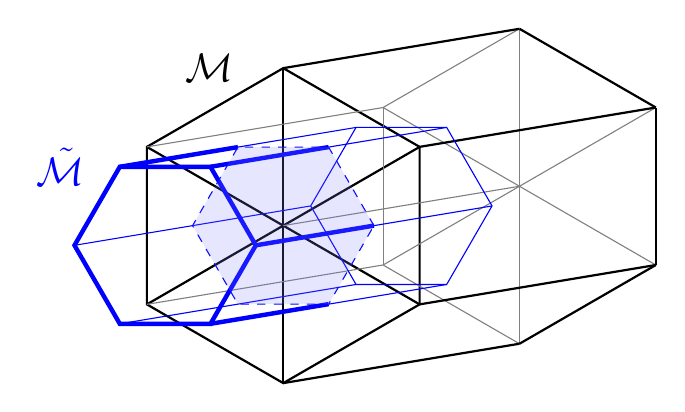
\begin{tikzpicture}
    \def\primalstyle{thick}
    \def\dualstyle{thick}
    \coordinate (P0) at (0cm, 0cm);
    \foreach \i in {1,2,...,6}
    {
    \coordinate (P\i) at ({60*\i-30}:2cm);
    \draw[\primalstyle] (P0) -- (P\i);
    }
    \draw[\primalstyle] (P1) -- (P2) node[left=5mm]{\Large $\mathcal{M}$} -- (P3) -- (P4) -- (P5) -- (P6) -- cycle;
    \begin{scope}[shift={(3cm,0.5cm)}]
        \coordinate (PP0) at (0cm, 0cm);
        \foreach \i in {1,2,...,6}
        {
        \coordinate (PP\i) at ({60*\i-30}:2cm);
        \draw[gray] (PP0) -- (PP\i);
        }
    \end{scope}
    
    \draw[\primalstyle] (PP1) -- (PP2);
    \draw[gray] (PP2) -- (PP3);
    \draw[gray] (PP3) -- (PP4);
    \draw[gray] (PP4) -- (PP5);
    \draw[\primalstyle] (PP5) -- (PP6);
    \draw[\primalstyle] (PP6) -- (PP1);
    
    \draw[gray] (P0) -- (PP0);
    \draw[\primalstyle] (P1) -- (PP1);
    \draw[\primalstyle] (P2) -- (PP2);
    \draw[gray] (P3) -- (PP3);
    \draw[gray] (P4) -- (PP4);
    \draw[\primalstyle] (P5) -- (PP5);
    \draw[\primalstyle] (P6) -- (PP6);
    
    \foreach \i in {1,2,...,6}
    {
    \coordinate (D\i) at ({60*\i-60}:{2./1.737});
    }
    \draw[dashed, blue] (D1) -- (D2) -- (D3) -- (D4) -- (D5) -- (D6) -- cycle;
    \begin{scope}[shift={(1.5,0.25)}]
        \foreach \i in {1,2,...,6}
        {
        \coordinate (DD\i) at ({60*\i-60}:{2./1.737});
        }
    \end{scope}
    \draw[blue] (DD1) -- (DD2) -- (DD3) -- (DD4) -- (DD5) -- (DD6) -- cycle;
    \draw[blue] (D1) -- (DD1);
    \draw[blue] (D2) -- (DD2);
    \draw[blue] (D3) -- (DD3);
    \draw[blue] (D4) -- (DD4);
    \draw[blue] (D5) -- (DD5);
    \draw[blue] (D6) -- (DD6);
    
    \begin{scope}[shift={(-1.5,-0.25)}]
        \foreach \i in {1,2,...,6}
        {
        \coordinate (DDD\i) at ({60*\i-60}:{2./1.737});
        }
    \end{scope}
    \draw[blue, ultra thick] (DDD1) -- (DDD2) -- (DDD3) node[left=3mm]{\textcolor{blue}{\Large $\Tilde{\mathcal{M}}$}} -- (DDD4) -- (DDD5) -- (DDD6) -- cycle;
    \draw[blue, ultra thick] (D1) -- (DDD1);
    \draw[blue, ultra thick] (D2) -- (DDD2);
    \draw[blue, ultra thick] (D3) -- (DDD3);
    \draw[blue] (D4) -- (DDD4);
    \draw[blue] (D5) -- (DDD5);
    \draw[blue, ultra thick] (D6) -- (DDD6);
    
    \fill[blue!50, opacity=0.2] (D1) -- (D2) -- (D3) -- (D4) -- (D5) -- (D6);
    
    \end{tikzpicture}
    \caption{Illustration of primal and dual meshes. Six primal cells, which are triangle prisms, are depicted by black and gray edges. One dual cell, which is a hexagon prism, is depicted by blue edges. The dashed hexagon represents the intersection of the dual cell and primal cells. This particular type of mesh composed of prisms is picked as a demonstration since it is used in our numerical experiments.}
    \label{fig:illustration_primal_dual}
\end{figure}
\subsection{Spatial semi-discretization} \label{sec:fit}
The FIT is established based on the integral form of Maxwell's equations:
\begin{align}
    &\oint_{\partial A} \mathbf{E} \cdot d\mathbf{s} \ = - \iint_A \frac{\partial \mathbf{B}}{\partial t} \cdot d\mathbf{A}, \label{equ:maxwell_int_faraday}\\
    &\oint_{\partial A} \mathbf{H} \cdot d\mathbf{s} \ = \iint_A \left(\frac{\partial \mathbf{D}}{\partial t} + \mathbf{J}\right) \cdot d\mathbf{A}, \label{equ:maxwell_int_ampere}\\
    &\oint_{\partial V} \mathbf{B} \cdot d\mathbf{A} = 0, \label{equ:maxwell_int_gauss_B}\\
    &\oint_{\partial V} \mathbf{D} \cdot d\mathbf{A} = \iiint_V \rho dV. \label{equ:maxwell_int_gauss_D}
\end{align}
where $A, V$ stand for any 2-D faces and 3-D cells in the spatial domain. These equations are consequence of curl theorem and divergence theorem, and correspond to the integral form of Faraday's law (\ref{equ:maxwell_int_faraday}), Ampere's law (\ref{equ:maxwell_int_ampere}) and Gauss's laws for magnetic flux (\ref{equ:maxwell_int_gauss_B}) and electric induction (\ref{equ:maxwell_int_gauss_D}). The fields are related by the material laws
\begin{align} \label{equ:maxwell_material_laws}
    \mathbf{B} = \mu_0 \mathbf{H},\ \ \ \mathbf{D} = \varepsilon_0 \mathbf{E}.
\end{align}

The discrete Maxwell system is obtained by applying and collecting the equations (\ref{equ:maxwell_int_faraday}) (\ref{equ:maxwell_int_gauss_B}) on each facet of the primal mesh $\mathcal{M}$ and the equations (\ref{equ:maxwell_int_ampere}) (\ref{equ:maxwell_int_gauss_D}) on each facet of the dual mesh $\Tilde{\mathcal{M}}$. We denote the vertices by $(P_i)_{i=1}^{N_P}$, $(\Tilde{P}_i)_{i=1}^{N_{\Tilde{P}}}$, edges by $(L_i)_{i=1}^{N_L}$, $(\Tilde{L}_i)_{i=1}^{N_{\Tilde{L}}}$, faces by $(A_i)_{i=1}^{N_A}$, $(\Tilde{A}_i)_{i=1}^{N_{\Tilde{A}}}$, and cells by $(V_i)_{i=1}^{N_V}$, $(\Tilde{V}_i)_{i=1}^{N_{\Tilde{V}}}$ where the ones with tilde belong to the dual mesh. Recall the duality property that $\mathcal{M}$ and $\mathcal{M}'$ interlaces with each other in the sense that each edge penetrates a face of the other mesh. This leads to $N_L = N_{\Tilde{A}}$ and $N_A = N_{\Tilde{L}}$\footnote{Note that here the influence of boundary is not considered.}. The equations (\ref{equ:maxwell_int_faraday}) to (\ref{equ:maxwell_int_gauss_D}) can be rewritten into

\begin{align}
    &\sum_{j:L_j\in\partial A_i} \underbrace{\int_{L_j} \mathbf{E} \cdot d\mathbf{s}}_{e_j} = - \frac{\partial}{\partial t} \underbrace{\iint_{A_i} \mathbf{B} \cdot d\mathbf{A}}_{b_i},\ \ \ i = 1,...,N_A, \label{equ:maxwell_grid_faraday} \\
    &\sum_{j:\Tilde{L}_j\in\partial \Tilde{A}_i} \underbrace{\int_{\Tilde{L}_j} \mathbf{H} \cdot d\mathbf{s}}_{h_j} = \frac{\partial}{\partial t} \underbrace{\iint_{\Tilde{A}_i} \mathbf{D} \cdot d\mathbf{A}}_{d_i} + \underbrace{\iint_{\Tilde{A}_i} \mathbf{J} \cdot d\mathbf{A}}_{j_i}, \ \ \ i = 1,...,N_{\Tilde{A}}, \label{equ:maxwell_grid_ampere}\\
    &\sum_{j:A_j\in \partial V_i} \iint_{A_j} \mathbf{B} \cdot d\mathbf{A} = 0,\ \ \ i = 1,..., N_V,\label{equ:maxwell_grid_gauss_B}\\
    &\sum_{j:\Tilde{A}_j \in \partial\Tilde{V}_i}\iint_{\Tilde{A}_j} \mathbf{D} \cdot d\mathbf{A} = \underbrace{\iiint_{\Tilde{V}_i} \rho dV}_{q_i},\ \ \ i = 1,...,N_{\Tilde{V}}. \label{equ:maxwell_grid_gauss_D}
\end{align}
For the sake of neat illustration, we temporarily neglect the boundary conditions which will be discussed later. As is indicated in (\ref{equ:maxwell_grid_faraday})(\ref{equ:maxwell_grid_ampere}) by the underbraces, the discrete variables are chosen as the integral quantities of field vectors on edges or faces. Packing these scalar quantities into vectors, we define
\begin{equation} \label{equ:fit_scale_vector}
    \mathbf{e} := (e_i)_{i=1}^{N_L},\ \ \mathbf{b} := (b_i)_{i=1}^{N_A}, \ \ \mathbf{h} := (h_i)_{i=1}^{N_{\Tilde{L}}}, \ \ \mathbf{d} := (d_i)_{i=1}^{N_{\Tilde{A}}}, \ \ \mathbf{j} := (j_i)_{i=1}^{N_{\Tilde{A}}}, \ \ \mathbf{q} := (q_i)_{i=1}^{N_{\Tilde{V}}}.
\end{equation}

The next step is to transform the discrete Maxwell system (\ref{equ:maxwell_grid_faraday}) to (\ref{equ:maxwell_grid_gauss_D}) into a set of algebraic equations. One should note that the sign of each scalar depends on the orientation of the facet on which it is integrated. To uniquely determine the meaning of these quantities, an \emph{internal orientation} is assigned to every facet of the primal mesh $\mathcal{M}$. This attribute defines the orientations of edges and outer normals of faces. Besides, since the application of curl theorem and divergence theorem entails the orientation relations of edge-to-face and face-to-volume respectively, another orientation attribute, \emph{induced orientation}, is introduced to specify this topology. An induced orientation of a $k$-dim facet $f$ with respect to a $(k+1)$-dim facet $f'$ that contains $f$ is determined by the internal orientation of $f'$ according to some rule. An example is shown in Fig. \ref{fig:illustration_external_orientation}.
These topological attributes are inherent for a mesh and can be set at will.

\begin{figure}
    \centering

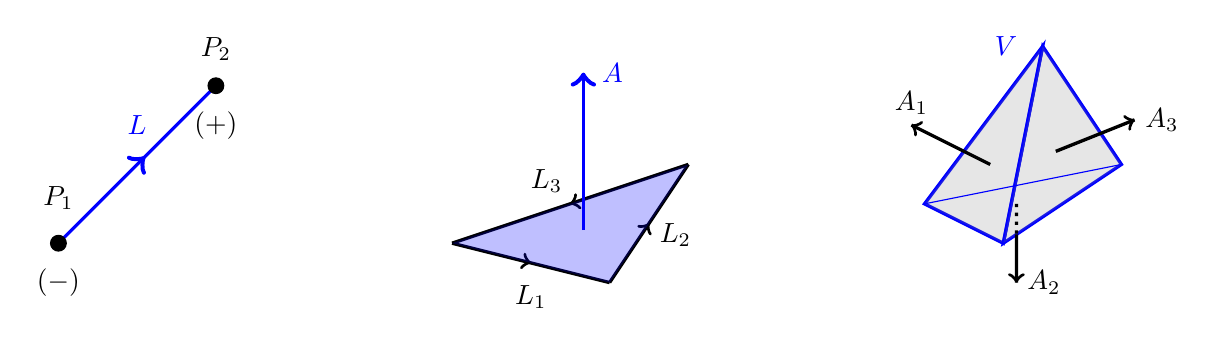
\begin{tikzpicture}
\coordinate (P1) at (0,0);
\coordinate (P2) at (2,2);
\draw[decoration={markings, 
    mark= at position 0.55 with {\arrow[scale=1.5]{to}}}
    ,postaction={decorate}, very thick, blue] (P1) -- (P2);
\node at (1,1.5) {\textcolor{blue}{$L$}};
\draw[fill=black] (P1) circle (0.1) node[above=3mm] {$P_1$} node[below=2mm] {$(-)$};
\draw[fill=black] (P2) circle (0.1) node[above=2mm] {$P_2$} node[below=2mm] {$(+)$};

\begin{scope}[shift={(5, 0)}]
\coordinate (Q1) at (0,0);
\coordinate (Q2) at (2cm, -0.5cm);
\coordinate (Q3) at (3cm, 1cm);
\draw[decoration={markings, 
    mark= at position 0.5 with {\arrow[scale=1]{to}}}
    , postaction={decorate}, very thick] (Q1) -- node[below=1.5mm]{$L_1$} (Q2);
    \draw[decoration={markings, 
    mark= at position 0.5 with {\arrow[scale=1]{to}}}
    , postaction={decorate}, very thick] (Q2) -- node[right,yshift=-1.5mm]{$L_2$} (Q3);
    \draw[decoration={markings, 
    mark= at position 0.5 with {\arrow[scale=1]{to}}}
    , postaction={decorate}, very thick] (Q3) -- node[above,xshift=-3mm] {$L_3$}(Q1);

\fill[blue, opacity=0.25] (Q1) -- (Q2) -- (Q3);
\draw[decoration={markings, 
    mark= at position 1 with {\arrow[scale=1.5]{to}}}
    , postaction={decorate}, very thick, blue](barycentric cs:Q1=1,Q2=1,Q3=1) -- ([shift={(0,2cm)}] barycentric cs:Q1=1,Q2=1,Q3=1) node[right,xshift=1mm] {\textcolor{blue}{$A$}}; 
\end{scope}

\begin{scope}[shift={(12,0)}]
\coordinate (S1) at (0,0);
\coordinate (S2) at (-1,0.5);
\coordinate (S3) at (1.5,1);
\coordinate (S4) at (0.5,2.5);
\draw[very thick, blue] (S1) -- (S2) -- (S4) -- cycle;
\fill[gray, opacity=0.2] (S1) -- (S2) -- (S4);
\draw[very thick, blue] (S1) -- (S3) -- (S4) -- cycle;
\fill[gray, opacity=0.2] (S1) -- (S3) -- (S4);
\draw[blue, thin] (S2) -- (S3);
\draw[decoration={markings, 
    mark= at position 1 with {\arrow[scale=1]{to}}}
    , postaction={decorate}, very thick] (barycentric cs:S1=1,S2=1,S4=1) -- ([shift={(-1,0.5)}] barycentric cs:S1=1,S2=1,S4=1) node[above] {$A_1$};
\coordinate (O1) at (barycentric cs:S1=1,S2=1,S3=1);
\coordinate (O2) at ([shift={(0,-1)}] barycentric cs:S1=1,S2=1,S3=1);
\coordinate (S)  at (intersection of O1--O2 and S1--S3);
\draw[very thick, dotted] (O1) -- (S);
\draw[decoration={markings, 
    mark= at position 1 with {\arrow[scale=1]{to}}}
    , postaction={decorate}, very thick] (S) -- (O2) node[right] {$A_2$};
\draw[decoration={markings, 
    mark= at position 1 with {\arrow[scale=1]{to}}}
    , postaction={decorate}, very thick] (barycentric cs:S1=1,S3=1,S4=1) -- ([shift={(1,0.4)}] barycentric cs:S1=1,S3=1,S4=1) node[right] {$A_3$} ;
\node at (S4) [left, xshift=-2mm] {\textcolor{blue}{$V$}};
\end{scope}
\end{tikzpicture}
    \caption{Illustration of induced orientations. As per our rule, the ending vertex of an edge is positively oriented while the starting point is negatively oriented; the orientations of edges with respect to a face obey the right-hand rule; a face of a volume are oriented with its outer normal. Note that the rule can be freely set.}
    \label{fig:illustration_external_orientation}
\end{figure}

With the aid of both internal and induced orientations, the facet-to-facet relations can be summarized by matrices containing only $\{-1,0,0\}$, which are called \emph{incidence matrices}. To describe the primal face-to-edge incidence relation, for instance, a sparse $N_A \times N_L$-matrix $\mathbb{C}$ is assembled whose $(i,j)$-entry is assigned $+1$ if the internal orientation of edge $L_j$ and its induced orientation with respect to face $A_i$ coincides; it is assigned $-1$ if two orientations are opposite; and assigned $0$ if $L_j$ is not a subset of the boundary of $A_i$. Discrete Faraday's law (\ref{equ:maxwell_grid_faraday}) is thus reformulated by:
\begin{equation*}
    \mathbb{C}\mathbf{e} = - \frac{\text{d}}{\text{d}t} \mathbf{b}.
\end{equation*}
As the incidence matrix $\mathbb{C}$ makes up the curl operator in a discrete manner, it is referred to as the \emph{discrete curl operator} for a certain primal mesh.

Given $\mathcal{M}$, the generation of $\Tilde{\mathcal{M}}$ is usually affiliated to $\mathcal{M}$ in terms of geometry, indexing, and topology. Although the latter two attributes can be defined with no dependence on $\mathcal{M}$, conventionally one specifies them relying on those of $\mathcal{M}$ for the sake of convenience in both formulation and implementation. Recall that primal edges (resp. faces) and dual faces (resp. edges) intersect in a one-to-one manner. Therefore, one can equate the index of a dual edge (resp. face) to that of its intersecting primal face (resp. edge). Furthermore, the internal orientation of a dual facet can be linked to that of its associated primal facet. With these constraints, discrete Ampere's law (\ref{equ:maxwell_grid_ampere}) can be reformulated into:
\begin{equation*}
    \Tilde{\mathbb{C}}\mathbf{h} = \frac{\text{d}}{\text{d}t} \mathbf{d} + \mathbf{j},
\end{equation*}
where $\Tilde{\mathbb{C}}$ is the dual face-to-edge incidence matrix of size $N_{\Tilde{A}} \times N_{\Tilde{L}}$, satisfying $\Tilde{\mathbb{C}} = \mathbb{C}^T$. 

In a similar way, discrete Gauss's laws (\ref{equ:maxwell_grid_gauss_B})(\ref{equ:maxwell_grid_gauss_D}) is rewritten into:
\begin{equation*}
    \mathbb{D}\mathbf{b} = 0, \ \ \ \  \Tilde{\mathbb{D}}\mathbf{d} = \mathbf{q},
\end{equation*}
with $\mathbb{D}$ being the primal cell-to-face incidence matrix of size $N_{V} \times N_{A}$, and $\Tilde{\mathbb{D}}$ being the dual cell-to-face incidence matrix of size $N_{\Tilde{V}} \times N_{\Tilde{A}}$. Since they serve as the discrete version of the div operator, they are also referred to as \emph{discrete div operator}. It is readily to be checked the following relations 
\begin{equation*}
    \mathbb{D}\mathbb{C} = 0, \ \ \ \ \Tilde{\mathbb{D}}\Tilde{\mathbb{C}} = 0,
\end{equation*}
which is the discrete version of the vector calculus $\nabla \cdot (\nabla \times u) = 0$.

Additionally, the grad operator at the discrete level can be constructed by edge-to-vertex incidence matrices $\mathbb{G}$ of size $N_L \times N_P$ and $\Tilde{\mathbb{G}}$ of size $N_{\Tilde{L}} \times N_{\Tilde{P}}$. Given an electric potential vector $\bm{\varphi}$ whose components are defined at primal vertices, for example, the edge voltage vector $\mathbf{e}$ can thus be computed by
\begin{equation*}
    \mathbf{e} = \mathbb{G}\bm{\varphi}.
\end{equation*}

The material laws (\ref{equ:maxwell_material_laws}) need to be reformulated within this framework. The relations between scalar vectors, in the form of $\mathbf{b} = \mathbb{M}_\mu \mathbf{h}$ and $\mathbf{d} = \mathbb{M}_\varepsilon \mathbf{e}$, are to be derived. In the simplest case where permittivity $\mu$ and permeability $\varepsilon$ are homogeneous in the domain, and the orthogonality\footnote{The edges of one mesh penetrate the faces of the other mesh in an orthogonal manner.} of ($\mathcal{M}, \Tilde{\mathcal{M}}$) pair is ensured, the material matrices are diagonal with entries 

\begin{equation*}
    \mathbb{M}_\mu[i,i] = \frac{\mu|A_i|}{|\Tilde{L}_i|}, \ \ \ \ \mathbb{M}_\varepsilon[i,i] = \frac{\varepsilon |\Tilde{A}_i|}{|L_i|},
\end{equation*}
where $|\cdot|$ means taking length or area.

To summarize, the FIT framework enables us to transform Maxwell’s equations into algebraic equations given the mesh pair ($\mathcal{M}, \Tilde{\mathcal{M}}$). The resulting system of algebraic equations is called Maxwell's Grid Equations (MGE). Let's put together the original form of the Maxwell system as well as the MGE:

\begin{minipage}{0.3\textwidth}
\begin{align*}
    \partial_t \mathbf{B} + \nabla \times \mathbf{E} &= 0, \\
    \partial_t \mathbf{D} - \nabla \times \mathbf{H} &= -\mathbf{J}, \\
    \nabla \cdot \mathbf{B} &= 0,  \\
    \nabla \cdot \mathbf{D} &= \rho, \\
    \mathbf{H} &= \mu^{-1} \mathbf{B}, \\
    \mathbf{D} &= \varepsilon \mathbf{E}. 
\end{align*}
\end{minipage}
\begin{minipage}{0.1\textwidth}
\centering
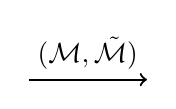
\begin{tikzpicture}
\draw[thick, -{to}] (0,0) -- node[above]{$(\mathcal{M}, \Tilde{\mathcal{M}})$} (1.5,0);
\end{tikzpicture}
\end{minipage}
\begin{minipage}{0.3\textwidth}
\begin{align*}
    \dot{\mathbf{b}} + \mathbb{C}\mathbf{e} &= 0 , \\
    \dot{\mathbf{d}} - \Tilde{\mathbb{C}}\mathbf{h} &= - \mathbf{j}, \\
    \mathbb{D}\mathbf{b} &= 0,  \\
    \Tilde{\mathbb{D}}\mathbf{d} &= \mathbf{q},  \\
    \mathbf{h} &= \mathbb{M}_\mu^{-1} \mathbf{b}, \\
    \mathbf{d} &= \mathbb{M}_{\varepsilon} \mathbf{e}. 
\end{align*}
\end{minipage}
\begin{minipage}{0.2\textwidth}
Topological relations:
\begin{align*}
    \Tilde{\mathbb{C}} = \mathbb{C}^T \\
    \mathbb{D}\mathbb{C} = 0 \\
    \Tilde{\mathbb{D}}\Tilde{\mathbb{C}} = 0
\end{align*}
\end{minipage}

\hfill

Note that this transformation does not introduce approximations \emph{except for} the discrete material laws. The essence of FIT lies in that the complexity of continuous electric and magnetic field quantities
is reduced to a finite number of well-defined discrete unknowns \citep{weiland_2003}.

\subsection{Boundary treatment} \label{sec:boundary_treatment}

So far we have not discussed the boundary treatment. In fact, in the formulation of MGE, no boundary of the spatial domain is taken into account and all the scalar vectors should be treated of infinite length. Yet in a computer simulation, the computational domain has to be bounded, and the introduction of boundary complicates the situation. Under the framework of FIT, the issue is twofold: 1) The staggered mesh doublet ($\mathcal{M}, \Tilde{\mathcal{M}}$) entails cut-off cells at the boundary such that the boundaries of both meshes match up. To close the cut-off cells, we need auxiliary facets and quantities attached to them. 2) The auxiliary edges might not be straight and the auxiliary faces might not be flat, which necessitates a versatile data structure to include such situations. The boundary effect is shown in Fig. \ref{fig:illustraion_dual_boundary}. How these auxiliary quantities are incorporated into the discrete system is explained in Chapter \ref{chap:numerical_experiments_in_3d} along with the specific case.

\begin{figure}
    \centering
    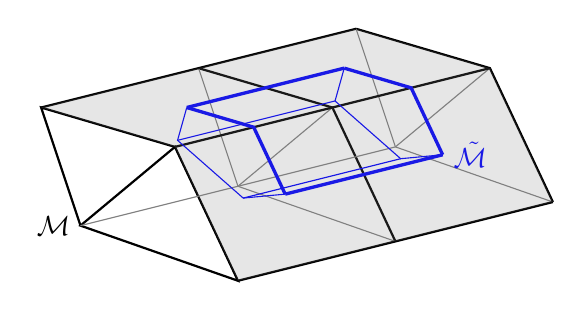
\begin{tikzpicture}
    \coordinate (A1) at (0,0);
    \coordinate (A2) at (2,-0.7);
    \coordinate (A3) at (1.2,1);
    \coordinate (A4) at (-0.5,1.5);
    \draw[thick] (A1) node[left] {$\mathcal{M}$} -- (A2) -- (A3) -- cycle;
    \draw[thick] (A1) -- (A4) -- (A3);
    \begin{scope}[shift={(2,0.5)}]
        \coordinate (B1) at (0,0);
        \coordinate (B2) at (2,-0.7);
        \coordinate (B3) at (1.2,1);
        \coordinate (B4) at (-0.5,1.5);
        \draw[thick] (B2) -- (B3) -- (B4);
        \draw[gray]  (B1) -- (B3);
        \draw[gray]  (B1) -- (B2);
        \draw[gray]  (B1) -- (B4);
    \end{scope}
    \begin{scope}[shift={(4,1)}]
        \coordinate (C1) at (0,0);
        \coordinate (C2) at (2,-0.7);
        \coordinate (C3) at (1.2,1);
        \coordinate (C4) at (-0.5,1.5);
        \draw[thick] (C2) -- (C3) -- (C4);
        \draw[gray]  (C1) -- (C3);
        \draw[gray]  (C1) -- (C2);
        \draw[gray]  (C1) -- (C4);
    \end{scope}
    \draw[thick] (A4) -- (B4) -- (C4);
    \draw[thick] (A3) -- (B3) -- (C3);
    \draw[thick] (A2) -- (B2) -- (C2);
    \draw[gray]  (A1) -- (C1);
    \coordinate (O1) at (barycentric cs:A3=1,B3=1);
    \coordinate (O2) at (barycentric cs:A3=1,B3=1,A4=1,B4=1);
    \coordinate (O5) at (barycentric cs:A3=1,B3=1,A2=1,B2=1);
    \draw[blue, very thick] (O2) -- (O1) -- (O5);
    \coordinate (O3) at (barycentric cs:A1=1,A3=1,A4=1,B1=1,B3=1,B4=1);
    \coordinate (O4) at (barycentric cs:A1=1,A2=1,A3=1,B1=1,B2=1,B3=1);
    \draw[blue] (O2) -- (O3) -- (O4) -- (O5);
    \coordinate (OO1) at ([shift={(2,0.5)}]O1);
    \coordinate (OO2) at ([shift={(2,0.5)}]O2);
    \coordinate (OO3) at ([shift={(2,0.5)}]O3);
    \coordinate (OO4) at ([shift={(2,0.5)}]O4);
    \coordinate (OO5) at ([shift={(2,0.5)}]O5);
    \draw[very thick, blue] (OO2) -- (OO1) -- (OO5) node[right] {\textcolor{blue}{$\Tilde{\mathcal{M}}$}};
    \draw[blue] (OO2) -- (OO3) -- (OO4) -- (OO5);
    \draw[very thick, blue] (O2) -- (OO2);
    %\draw[very thick, blue] (O1) -- (OO1);
    \draw[very thick, blue] (O5) -- (OO5);
    \draw[blue] (O3) -- (OO3);
    \draw[blue] (O4) -- (OO4);
    \fill[gray,opacity=0.2] (A4) -- (A3) -- (C3) -- (C4);
    \fill[gray,opacity=0.2] (A3) -- (A2) -- (C2) -- (C3);
    \end{tikzpicture}
    \caption{Illustration of a cut-off dual cell at the boundary. Compared to the interior case, the dual cells at boundary are cut off. Besides, an extra dual face (with thick blue edges) as well as their edges are supplemented to close the dual mesh. Note that this supplementary face is not necessarily flat, and its edges are not necessarily straight, as is shown here.}
    \label{fig:illustraion_dual_boundary}
\end{figure}

\section{Interpolation of electromagnetic quantities} \label{sec:interpolation}
The coupling of the two subsystems is bidirectional, in the sense that the Maxwell system impacts the Euler system through the Lorentz force while the latter provides information about charges and currents to the former. Since the currents, as is indicated by (\ref{equ:maxwell_grid_ampere}), are defined at dual faces and appear as mass fluxes in the fluid equations, the Euler system is discretized on the dual mesh. Therefore, an issue occurs because the component-wise electromagnetic fields are required to compute the Lorentz force inside the dual cells whereas the Maxwell system can only provide the integral form due to the nature of FIT. Hence the interpolation from the integral form on either edges or faces to the vector form at the cell center has to be tackled.

The problem is summarized as:
\begin{itemize}
    \item[-] Given the flux at each face of a polyhedron, reconstruct the vector field at the cell center;
    \item[-] Given the projection at each edge of a polyhedron, reconstruct the vector field at the cell center. 
\end{itemize}
We adopt the principle of least square fitting, and try to reconstruct the \emph{constant} vector field inside each cell. Specifically, assuming a polyhedral cell with $k$ faces with areas $\{A_i\}_{i=1}^k$, normal vectors $\{\mathbf{n}_i\}_{i=1}^k$ and fluxes $\{f_i\}_{i=1}^k$, one wants to find a vector $\mathbf{h}$ satisfying 
\begin{equation*}
    \mathbf{h} = \argmin_{h\in \mathbb{R}^3} \sum_{i=1}^k(A_i\mathbf{h} \cdot \mathbf{n}_i - f_i)^2.   
\end{equation*}
The solution can be easily expressed as
\begin{equation*}
    \mathbf{h} = (\mathbb{K}^T\mathbb{K})^{-1}\mathbb{K}^T\mathbf{f},
\end{equation*}
where
\begin{equation*}
    \mathbb{K} = [A_1\mathbf{n}_1, A_2\mathbf{n}_2, \cdots, A_k\mathbf{n}_k]^T,\ \ \ \mathbf{f} = [f_1, f_2, \cdots, f_k]^T,
\end{equation*}
and each vector in $\mathbb{R}^3$ is treated as a column vector.

The interpolation based on the integral quantities on edges can be done similarly, namely to find a constant vector field that minimizes the square error. This approach amounts to a first-order interpolation in the sense that a constant vector field can be precisely reconstructed. Assembling the local interpolation of each dual cell, we end up getting the global interpolation relation
\begin{equation}
    \mathbf{E} = \Tilde{\mathbb{R}}_E\mathbf{e},
    \ \ \ \ 
    \mathbf{B} = \Tilde{\mathbb{R}}_B\mathbf{b},
\end{equation}
where $\mathbf{e}, \mathbf{b}$ are electric voltage vector and magnetic flux vector defined in (\ref{equ:fit_scale_vector}); $\mathbf{E} := (\mathbf{E}_i)_{i=1}^{N_{\Tilde{V}}}$ and $\mathbf{B} := (\mathbf{B}_i)_{i=1}^{N_{\Tilde{V}}}$ are $N_{\Tilde{V}} \times 3$ matrices stacking the interpolated $\mathbf{E}$-field and $\mathbf{B}$-field at each dual cell center; $\Tilde{\mathbb{R}}_E$ and $\Tilde{\mathbb{R}}_B$ are thus rank-3 tensors that perform interpolation.

The problem of the reconstruction of vector fields on unstructured meshes is a widely studied topic. Apart from the least-square method, other methods include Perot's method \citep{perot_2000}, finite-element-based methods, etc., which potentially can achieve higher-order accuracy. See \cite[][sec. 3.4.4]{fuchs_2021} and the references therein.  

\chapter{Asymptotic-preserving Schemes for Euler-Maxwell System}
The objective of AP schemes is to solve problems over different regimes, that is, problems with a huge gap in a certain characteristic scale $\lambda$. An AP scheme expects to provide a uniformly working discretization for arbitrary value of $\lambda$. To this end, two central issues must be solved: first, the dependence of a stability-induced constraint on $\lambda$ has to be alleviated; second, $\lambda \rightarrow 0$ usually poses a singular perturbation problem, and the limiting scheme is supposed to remain valid and consistent to the limiting model.

A plasma is a multi-scale system that involves several scales, e.g. the wave speeds of electromagnetic fields and plasma fluids, and the plasma thermal speed that impacts its response to an external electromagnetic field. The identification of the impact of different characteristic scales is realized by rescaling the equations. The scale of interest in this work is the Debye length $\lambda_D$ that has a strong connection with the quasi-neutrality of plasma.

This chapter is organized as follows. First, we define several typical quantities relying on which the Euler-Maxwell system is rescaled. By making assumptions on the magnitude relations between these typical quantities, the parametrization of the system is limited to the dimensionless Debye length $\lambda$ and the quasi-neutral behavior can thus be identified. Afterward comes the presentation of an AP scheme. The asymptotic stability and consistency, namely the two properties as are defined in definition \ref{def:ap}, are discussed for this scheme. At last, we talk about two issues, namely boundary conditions and the presence of an insulating domain, that hinders the construction of AP schemes in the way that they could undermine the well-posedness of the problem in the limiting case.  

\section{Rescaling of Euler-Maxwell system} \label{sec:rescaling}
The multi-scale nature of the Euler-Maxwell system is revealed by defining different dimensionless parameters. In particular, the quasi-neutrality approximation is clarified. The rescaling procedure mostly sticks to that of \cite{degond_2017}.

First, typical values for each quantity, as well as the characteristic length and time scale are specified. Rescaled by these values, the magnitude of each term of the equations can be compared according to the presumption on the magnitude of these typical values. We define $\overline{x}$ and $\overline{t}$ as space and time scale of interest, by which the reference velocity $\overline{v}$ is defined as $\overline{x}/\overline{t}$. The typical magnitudes of electromagnetic fields are $\overline{E}$ and $\overline{B}$. The typical magnitudes of fluid quantities are denoted by $\overline{u}$ for plasma drift velocity, $\overline{n}$ for plasma number density, $\overline{T}$ for plasma temperature. On top of that, the typical pressure is set $\overline{n}k_B\overline{T}$ with $k_B$ being the Boltzmann constant; the typical value for the specific total energy and enthalpy is set $\overline{u}^2$. Together with the physical parameters, namely, permittivity $\varepsilon_0$, permeability $\mu_0$, light speed $c^2 = (\varepsilon_0\mu_0)^{-1}$, Boltzmann constant $k_B$, the elementary charge $e$, and ion mass $m_i$, the following dimensionless parameters are induced,
\begin{align*} 
    \xi &:= \frac{\overline{v}}{c} \text{ the velocity of interest to the light speed}, &\\
    \zeta &:= \frac{\overline{u}}{\overline{v}} \text{ the plasma velocity to the speed of interest}, &\\
    M &:= \frac{\overline{u}}{v_{th,i}} \text{ the plasma drift velocity to the thermal speed of ions, where } v_{th,i} := \left(\frac{k_B \overline{T}}{m_i}\right)^{1/2}, &\\
    \eta &:= \frac{e\overline{E}\overline{x}}{m_i\overline{u}^2} \text{ the electric energy to the kinetic energy of ions}, &\\
    \beta &:= \frac{\overline{v}\overline{B}}{\overline{E}} \text{ the induced electric field to the total electric field}, &\\
    \lambda &:= \frac{\lambda_D}{\overline{x}} \text{ the dimensionless Debye length, where }\lambda_D := \left(\frac{\varepsilon_0k_B\overline{T}}{e^2\overline{n}}\right)^{1/2}, &\\
    \varepsilon_*^2 &:= \frac{m_*}{m_i} \text{ the species mass ratio to the ion mass},\ \  * \in \{i,e,n,\cdots\}, &\\
    g &:= \frac{1}{\overline{n}\lambda_D^3} \text{ the plasma parameter\footnotemark}.&
\end{align*}
\footnotetext{It is basically the reciprocal of the number of particles per Debye sphere, see \cite[][sec. 1.1]{gibbon2020}. Classical plasma theory assumes $g \ll 1$.} 

The Euler-Maxwell system (\ref{equ:maxwell_faraday}) to (\ref{equ:euler_}) is readily to be rescaled by nondimensionalizing each quantity with respect to its typical value. By abuse of notation, the dimensionless quantities have the same symbol with their original ones without incurring any ambiguity. For simplicity, we only consider the collision terms, namely $\Gamma_* = 0, \mathbf{R}_* = \mathbf{R}_*^\text{coll}, Q_* = 0$ in (\ref{equ:euler_}), while neglecting other effects. The rescaled Euler-Maxwell system reads
\begin{align}
    \beta \partial_t \mathbf{B} + \nabla \times \mathbf{E} &= 0, \label{equ:maxwell_faraday_rescalling} \\ 
    \lambda^2 \partial_t \mathbf{E} - \frac{\beta \lambda^2}{\xi^2}\nabla \times \mathbf{B} &= - \frac{\zeta}{\eta M^2}\mathbf{J}, \label{equ:maxwell_ampere_rescalling} \\
    \nabla \cdot \mathbf{B} &= 0,  \label{equ:maxwell_gauss_B_rescalling}\\
    \lambda^2 \eta M^2 \nabla \cdot \mathbf{E} &= \rho, \label{equ:maxwell_gauss_D_rescalling} \\
    \partial_t
    \begin{bmatrix}
    n_* \\
    n_* \mathbf{u}_* \\
    n_* e_*
    \end{bmatrix}
    + \nabla \cdot
    \begin{bmatrix}
    \zeta n_* \mathbf{u}_* \\
    \zeta n_* \mathbf{u}_* \otimes \mathbf{u}_* + \zeta M^{-2} \varepsilon_*^{-2} p_*\mathbb{I} \\
    \zeta n_* h_* \mathbf{u}_*
    \end{bmatrix}
    &=
    \begin{bmatrix}
    0 \\
    \eta \zea \varepsilon_*^{-2} q_* n_*\mathbf{E} + \eta \zeta^2 \beta \varepsilon_*^{-2} q_* n_* \mathbf{u}_* \times \mathbf{B} \\
    \zeta \eta \varepsilon_*^{-2} \mathbf{J}_* \cdot \mathbf{E}
    \end{bmatrix} +
    \begin{bmatrix}
    0 \\
    \varepsilon_*^{-2}\mathbf{R}_*^{\text{coll}} \\
    0 
    \end{bmatrix}, \label{equ:euler_rescalling}
\end{align}
where the equation of state becomes $e_* = \frac{1}{2}|\mathbf{u_*}|^2 + M^{-2}\frac{p_*}{\epsilon^2_* n_* (\gamma - 1)}$ and $h_* = e_* + M^{-2}\frac{p_*}{\epsilon^2_* n_*}$. For a fully-ionized gas, we have the original expression of $\mathbf{R}_*^{\text{coll}}$ in (\ref{equ:collision}), and its rescaled expression becomes
\begin{equation*}
    \mathbf{R}_i^{\text{coll}} = \frac{Z\text{ln}\Lambda}{16\pi}g\lambda^{-1}M^{-1}\varepsilon_en_en_i(\mathbf{u}_i - \mathbf{u}_e). 
\end{equation*}

Following the assumption in \cite{degond_2017}, the reference speed $\overline{v}$ is of the same scale with the plasma speed $\overline{u}$ and the thermal speed $v_{th,i}$ whereas it is much smaller than the light speed $c$. To study the quasi-neutral regime, the dimensionless Debye length $\lambda$ is an asymptotic parameter ranging in $[0,1]$. It is assumed that $\alpha$ has the same magnitude as $\lambda$, and $\eta$ and $\beta$ are of order one. 

Special treatment is needed for the collision term. One would notice the inverse proportionality to $\lambda$, which would introduce a singular perturbation to the Euler system as $\lambda \rightarrow 0$. However, the validity of such a collision model is doubtful when $\lambda \rightarrow 0$. From the physical viewpoint, the shielding effect characterized by Debye length $\lambda$ makes the impact parameter no larger than $\lambda$. The $\lambda \rightarrow 0$ limit implies that the collisions happen in the atomic length scale, in which quantum-mechanical effects must be taken into effect \citep{frank_1972}. Therefore, for simplicity, we decide to assume $g \sim \lambda$ and keep the prefactor of collision term constant $\alpha^{\text{coll}}$ throughout the simulation\footnote{The reasonableness of this assumption is questionable.}.  

In summary, we make the following choices
\begin{align*}
    \xi \sim g \sim \lambda \in [0,1], \ \ \ \zeta \sim M \sim \eta \sim \beta \sim \mathcal{O}(1).
\end{align*}


Under such assumptions on these dimensionless parameters, the rescaled Euler-Maxwell system is simplified into a parametrized system with the dimensionless Debye length $\lambda$ being the asymptotic parameter
\begin{align}
    \partial_t \mathbf{B} + \nabla \times \mathbf{E} &= 0, \label{equ:maxwell_faraday_rescaled} \\ 
    \lambda^2 \partial_t \mathbf{E} - \nabla \times \mathbf{B} &= - \mathbf{J}, \label{equ:maxwell_ampere_rescaled} \\
    \nabla \cdot \mathbf{B} &= 0,  \label{equ:maxwell_gauss_B_rescaled}\\
    \lambda^2 \nabla \cdot \mathbf{E} &= \rho, \label{equ:maxwell_gauss_D_rescaled} \\
    \partial_t
    \begin{bmatrix}
    n_* \\
    n_* \mathbf{u}_* \\
    n_* e_*
    \end{bmatrix}
    + \nabla \cdot
    \begin{bmatrix}
    n_* \mathbf{u}_* \\
    n_* \mathbf{u}_* \otimes \mathbf{u}_* + \varepsilon_*^{-2} p_*\mathbb{I} \\
    n_* h_* \mathbf{u}_*
    \end{bmatrix}
    &=
    \begin{bmatrix}
    0 \\
    \varepsilon_*^{-2} q_* n_* (\mathbf{E} + \mathbf{u}_* \times \mathbf{B}) \\
    \varepsilon_*^{-2} \mathbf{J}_* \cdot \mathbf{E}
    \end{bmatrix}+
    \begin{bmatrix}
    0 \\
    \varepsilon_*^{-2}\mathbf{R}_*^{\text{coll}} \\
    0 
    \end{bmatrix}, \label{equ:euler_rescaled}
\end{align}
with the equation of state $e_* = \frac{1}{2}|\mathbf{u_*}|^2 + \frac{p_*}{\varepsilon^2_* n_* (\gamma - 1)}$ and $h_* = e_* + \frac{p_*}{\varepsilon^2_* n_*}$. For a fully-ionized gas with only ions and electrons, 
\begin{equation} \label{equ:collision_rescaled} 
    \mathbf{R}_i^{\text{coll}} = \alpha^{\text{coll}}n_en_i(\mathbf{u}_i - \mathbf{u}_e) = - \mathbf{R}_e^{\text{coll}}.
\end{equation}


Although the rescaling of the equations involves considerable physical intuitions on the decision of typical values and their magnitudes, which is crucial to reach a physically meaningful problem, we are now in a position to forget this reasoning, and focus on the singular perturbation problem parameterized by $\lambda$. The rescaling enables us to identify the magnitude of each term of the equations, which is revealed by the prefactor polynomial of $\lambda$. The consequence of vanishing $\lambda$, namely the quasi-neutrality, will be discussed in the next section.

\section{Quasi-neutral limit} \label{sec:quasi-neutral_limit}
As is already discussed in section \ref{sec:quasi-neutrality}, the quasi-neutrality, being an important character of plasmas, refers to the fact that the net charge of the free electrons and ions in plasmas cancel out over an area of the same order as the Deybe length $\lambda_D$. When the typical length scale $\overline{x}$ is of magnitudes larger than $\lambda_D$, the condition $\rho = 0$ can be approximately satisfied.

Such behavior is clearly explained through the rescaled Euler-Maxwell system (\ref{equ:maxwell_faraday_rescaled}) to (\ref{equ:euler_rescaled}). By formally taking dimensionless Debye length $\lambda$ to zero\footnote{The convergence of the solutions as $\lambda$ tending to zero is discussed in \cite[][chap. 2]{remi_2014}}, the Maxwell system becomes 
\begin{align}
    \partial_t \mathbf{B} + \nabla \times \mathbf{E} &= 0, \label{equ:maxwell_faraday_limit} \\ 
    - \nabla \times \mathbf{B} &= - \mathbf{J}, \label{equ:maxwell_ampere_limit} \\
    \nabla \cdot \mathbf{B} &= 0,  \label{equ:maxwell_gauss_B_limit}\\
     0 &= \rho. \label{equ:maxwell_gauss_D_limit}
\end{align}
One can notice that the quasi-neutral condition (\ref{equ:maxwell_gauss_D_limit}) is the consequence of taking $\lambda = 0$ in Gauss's law for electric field (\ref{equ:maxwell_gauss_D_rescaled}). Like the non-neutral case, Gauss's laws (\ref{equ:maxwell_gauss_B_limit}) (\ref{equ:maxwell_gauss_D_limit}) are the consequence of (\ref{equ:maxwell_faraday_limit}) (\ref{equ:maxwell_ampere_limit}) provided (\ref{equ:maxwell_gauss_B_limit}) (\ref{equ:maxwell_gauss_D_limit}) are satisfied at the initial time.  

The vanishing time derivative of $\mathbf{E}$-field is an indicator of the singular perturbation nature of the quasi-neutral model. To be specific, in the non-neutral model the $\mathbf{E}$-field evolves with time whereas in the quasi-neutral model it responds instantaneously to other quantities according to the constraint (\ref{equ:maxwell_ampere_limit}). To make it clear, we replace the equation (\ref{equ:maxwell_ampere_rescaled}) by the sum of the curl of (\ref{equ:maxwell_faraday_rescaled}) and the time-derivative of (\ref{equ:maxwell_ampere_rescaled}). Meanwhile exploiting the momentum equation in (\ref{equ:euler_rescaled}) to express $\partial_t\mathbf{J}$, we end up getting the reformulated Maxwell's equations
\begin{align}
    \partial_t \mathbf{B} + \nabla \times \mathbf{E} &= 0, \label{equ:maxwell_faraday_reform}\\
    \lambda^2\partial_t^2 \mathbf{E} + \nabla \times \nabla \times \mathbf{E} &= - a\mathbf{E} - \mathbf{b}, \label{equ:maxwell_ampere_reform}\\
    \nabla \cdot \mathbf{B} &= 0,  \label{equ:maxwell_gauss_B_reform}\\
    \lambda^2\nabla \cdot \mathbf{E} &= \rho, \label{equ:maxwell_gauss_D_reform}
\end{align}
where
\begin{equation*}
    a = \sum_*\varepsilon_*^{-2}q_*^2n_*, \ \ \ \mathbf{b} = \sum_* \epsilon_*^{-2}q_*^2n_*\mathbf{u}_*\times\mathbf{B} - q_*\nabla\cdot(n_* \mathbf{u}_* \otimes \mathbf{u}_* + \varepsilon_*^{-2}p_*\mathbb{I}).
\end{equation*}
It is easy to check that (\ref{equ:maxwell_faraday_reform}) to (\ref{equ:maxwell_ampere_reform}) is equivalent to (\ref{equ:maxwell_faraday_rescaled}) to (\ref{equ:maxwell_gauss_D_rescaled}) as soon as (\ref{equ:maxwell_ampere_rescaled}) is satisfied at the initial time. The equation (\ref{equ:maxwell_ampere_reform}) implies the shift from the hyperbolic nature to the elliptic nature of the $\mathbf{E}$-field as $\lambda\rightarrow0$. One of the key aims of designing an AP scheme is to reproduce this shift at the discrete level.

\section{AP schemes}
In this section, we present the full discretization with AP property. The general approach for spatial discretizations of both the Euler and Maxwell's equations has been introduced in chapter \ref{chap:discretization_euler_maxwell}. As stability is a central issue for the AP property, this section is mostly devoted to the time discretization of the Euler-Maxwell system.

We want to first recall the objective of AP schemes and make clear the direction to proceed towards. By definition \ref{def:ap}, the stability condition that does not depend on $\lambda$ and the consistency of the limit scheme with the quasi-neutral system have to be fulfilled. Furthermore, what is desired for the numerical treatment of Maxwell's equations is that Gauss's law is satisfied at the discrete level. To sum up, the following properties of the constructed scheme are to be realized:

\begin{itemize}
    \item[I] stable regardless of the value of $\lambda$;
    \item[II] the limit scheme by taking $\lambda = 0$ is valid\footnote{By ``valid" we mean the scheme is a valid recursion such that the state at $t^{m+1}$ can be \emph{uniquely} computed by that at $t^m$.} and consistent to its continuous counterpart (\ref{equ:maxwell_faraday_limit}) to (\ref{equ:maxwell_gauss_D_limit});
    \item[III] Gauss's law (\ref{equ:maxwell_gauss_D_rescaled}) is fulfilled at the discrete level for any $\lambda$. \label{condition3}
\end{itemize}

Given the mesh pair $(\mathcal{M}, \Tilde{\mathcal{M}})$, Maxwell's equations are handled by the FIT framework while FVM is applied to Euler equations on the dual mesh 
$\Tilde{\mathcal{M}}$. Naturally extending the AP scheme for 1D two-fluid plasma proposed in \cite{degond_2012} to which the detailed constructing procedure should be referred, we straightforwardly present the full-discretization scheme for 3D multi-species plasma:

\begin{align}
    \delta_m^{-1} (\mathbf{b}^{m+1} - \mathbf{b}^{m}) \hspace{0.4cm}&\;+\; \hspace{1.5cm}\mathbb{C}\textcolor{blue}{\mathbf{e}^{m+1}}\hspace{1.25cm}=\; 0, \label{equ:maxwell_faraday_ap}\\
    \lambda^2\delta_m^{-1}(\mathbf{d}^{m+1} - \mathbf{d}^m) \hspace{0.4cm}&\;-\; \hspace{1.5cm}\Tilde{\mathbb{C}}\textcolor{blue}{\mathbf{h}^{m+1}} \hspace{1.22cm}=\; - \textcolor{blue}{\mathbf{j}^{m+1}}, \label{equ:maxwell_ampere_ap}\\
    \delta_m^{-1}(\mathbf{U}_{*,k}^{m+1} - \mathbf{U}_{*,k}^{m}) \hspace{0.10cm}&\;+\;  \frac{1}{|\Tilde{V}_k|}\sum_{j:\Tilde{A}_j\in\partial\Tilde{V}_k}|\Tilde{A}_j|\textcolor{blue}{\overline{\mathbf{F}}_{*,j}^{m+1/2}} \hspace{0.05cm}=\; \textcolor{blue}{\mathbf{RHS}_{*,k}^{m+1/2}}, \label{equ:euler_ap}
\end{align}
where 
\begin{align}
    \mathbf{U}_{*,k}^{m} &=
    \begin{bmatrix}
    n_* \\
    n_* \mathbf{u}_* \\
    n_* e_*
    \end{bmatrix}^m_k, \\
    \overline{\mathbf{F}}_{*,j}^{m+1/2} &=
    \begin{bmatrix}
    f^{m+1}_{n,*,j} \\
    \bm{f}^m_{u,*,j} \\
    f^m_{e,*,j} 
    \end{bmatrix}
    = 
    \begin{bmatrix}
    \frac{1}{2}\left[\textcolor{blue}{(nu_{\bot})_{*,k}^{m+1}} + \textcolor{blue}{(nu_{\bot})_{*,k+1}^{m+1}}\right] - \frac{1}{2}s^m_{*,k+1/2}(n_{*,k+1}^m - n_{*,k}^m) \\
    \frac{1}{2}\left[(nu_{\bot}\mathbf{u})^m_{*,k} + (nu_{\bot}\mathbf{u})^m_{*,k+1} + p_{*,k}^m\mathbf{n}_j + p_{*,k+1}^m\mathbf{n}_j\right] - \frac{1}{2}s^m_{*,k+1/2}\left[(n\mathbf{u})^m_{*,k+1} - (n\mathbf{u})^m_{*,k}\right] \\
    \frac{1}{2}\left[(nhu_\bot)^m_{*,k} + (nhu_\bot)^m_{*,k+1}\right] - \frac{1}{2}s^m_{*,k+1/2}\left[(ne)^m_{*,k+1} - (ne)^m_{*,k}\right]
    \end{bmatrix}, \label{equ:flux_ap}\\
    \mathbf{RHS}_{*,k}^{m+1/2} &=
    \begin{bmatrix}
    0 \\
    \varepsilon_*^{-2}q_*\left[n_*^m\textcolor{blue}{\mathbf{E}^{m+1}} + (n\mathbf{u})^m_*\times\mathbf{B}^m\right] \\
    \varepsilon_*^{-2}q_*(n\mathbf{u})^m_* \cdot \textcolor{blue}{\mathbf{E}^{m+1}}
    \end{bmatrix}_k +
    \begin{bmatrix}
    0 \\
    \varepsilon_*^{-2}\textcolor{blue}{\mathbf{R}_{*,k}^{\text{coll},m+1}} \\
    0
    \end{bmatrix}, \label{equ:rhs_ap}\\
    \mathbf{R}_{*,k}^{\text{coll},m+1} &= 
    \begin{cases}
    \alpha^\text{coll}\left[n_{e,k}^m\textcolor{blue}{(n\mathbf{u})^{m+1}_{i,k}} - n_{i,k}^m\textcolor{blue}{(n\mathbf{u})^{m+1}_{e,k}}\right] \text{  if  } * = e \\
    \alpha^\text{coll}\left[n_{i,k}^m\textcolor{blue}{(n\mathbf{u})^{m+1}_{e,k}} - n_{e,k}^m\textcolor{blue}{(n\mathbf{u})^{m+1}_{i,k}}\right] \text{  if  } * = i
    \end{cases}  \\
    \mathbf{j}^{m+1} &= \left(\sum_*\pm q_*\textcolor{blue}{f^{m+1}_{n,*,j}}|\Tilde{A}_j|\right)_{j=1}^{N_{\Tilde{A}}}, \label{equ:current_ap}\\
    \mathbf{d}^m &= \mathbb{M}_\varepsilon \mathbf{e}^m, \ \ \ \mathbf{h}^m = \mathbb{M}_\mu^{-1} \mathbf{b}^m. \label{equ:material_law}
\end{align}
In the above scheme, the superscript $m$ indicates the number of iterations, and the quantities with superscript $m+1/2$ implies its dependency on the quantities at both $m$-th and $(m+1)$-th iterations; $\delta_m$ is the time step size for the $m$-th iteration. The numerical flux (\ref{equ:flux_ap}), where $u_\perp$ stands for the velocity component normal to the dual face $\Tilde{A}_j$, is just the application of the generic Rusanov flux (\ref{equ:rusanov-flux-3d}) on the Euler equations, see also the expression (\ref{equ:rusanov_flux_euler}) in the appendix.  

By abuse of notations, quantities with subscript $k+1$ are associated with the adjacent cell of $\Tilde{V}_k$ with respect to $\Tilde{A}_j$, which should not be confused with its real index. $\mathbf{n}_j$ is the outer normal of $\Tilde{A}_j$ as a face of $\Tilde{V}_k$. Since the equations have been rescaled into the dimensionless form, the material matrices $\mathbb{M}_\varepsilon = \text{diag}(\{|\Tilde{A}_i|/{|L_i|}\}_i)$, $\mathbb{M}_\varepsilon = \text{diag}(\{{|A_i|}/{|\Tilde{L}_i|}\}_i)$ now only depend on the meshes. 

Recall that the discrete Euler system (\ref{equ:euler_ap}) is defined on the dual mesh $\Tilde{\mathcal{M}}$, and hence $\mathbf{E}^{m+1}$ and $\mathbf{B}^m$ in (\ref{equ:rhs_ap}) are the interpolated vector fields at dual cell center as is illustrated in section \ref{sec:interpolation}. The $\pm$ in (\ref{equ:current_ap}) arises from the fact that the direction of numerical fluxes is determined by the outer normal of each cell whereas each component in $\mathbf{j}^{m+1}$ is defined to be aligned with the internal orientation of the dual face it associates with. Hence a flip of the sign may be necessary. 

First, we would like to discuss the necessity of the implicit terms (highlighted in blue color). The implicit treatment of electric field in (\ref{equ:rhs_ap}) is a must to ensure stability and is justified in \cite{fabre_1992} for the Euler-Poisson system. It is reasonable to infer that it applies equally to the Euler-Maxwell system. To guarantee Gauss's law at the discrete level, the current in (\ref{equ:maxwell_ampere_ap}), as well as the mass flux in (\ref{equ:flux_ap}), must be at the same implicit level. The reformulated Ampere's law (\ref{equ:maxwell_ampere_reform}) gives us some clue that in the quasi-neutral case the right-hand side, arising from the electric current, must be implicit to lead to a valid and unique time-stepping. Furthermore, we stress that the current (\ref{equ:current_ap}) is evaluated by the numerical mass flux rather than its original definition $\sum_*n_*q_*\mathbf{u}_*$ for the sake of consistency to the discrete Gauss's law. The implicitness of the electric field in (\ref{equ:maxwell_faraday_ap}) and the magnetic flux in (\ref{equ:maxwell_ampere_ap}) is necessary for unconditional stability with respect to $\lambda$, as is demonstrated by \cite{degond_2012} through a linearized analysis. The implicitness of the friction term is owing to the stiffness incurred from a potentially large value of $\varepsilon^{-2}_*\alpha^\text{coll}$.

Now we deduce the limiting scheme and check its validity and consistency. By formally setting $\lambda = 0$ in the AP scheme (\ref{equ:maxwell_faraday_ap}) to (\ref{equ:euler_ap}), the equation for evolving the electric edge voltages (\ref{equ:maxwell_ampere_ap}) degenerates into a constraint that should be satisfied at each step, namely
\begin{equation*}
     \Tilde{\mathbb{C}}\mathbb{M}_\mu^{-1}\mathbf{b}^{m+1} = - \mathbf{j}^{m+1}.
\end{equation*}
We want to check the consistency of the limiting scheme with the quasi-neutral model, and especially to check if the constraint (\ref{equ:maxwell_ampere_reform}) when $\lambda = 0$ is correctly discretized. To that end, we mimic the procedure to derive (\ref{equ:maxwell_ampere_reform}) in a discrete way, which leads to
\begin{equation*}
    (\Tilde{\mathbb{C}}\mathbb{M}_\mu^{-1}\mathbb{C}\mathbf{e}^{m+1})_j / |\Tilde{A}_j| = - \frac{1}{2}(a_{j,k}^m\mathbf{E}^{m+1}_{j,k} + a_{j,k+1}^m\mathbf{E}^{m+1}_{j,k+1})\cdot \mathbf{n}_j - \frac{1}{2}(\mathbf{b}_{j,k}^m + \mathbf{b}_{j, k+1}^m) \cdot \mathbf{n}_j - \pi_j^m,
\end{equation*}
where
\begin{align*}
    a_{j,k}^m &= \sum_*\pm\varepsilon_*^{-2}q_*^2n^m_{*,k}, \\
    \mathbf{b}_{j,k}^m &= \sum_*\pm\varepsilon_*^{-2}q_*\left[(n\mathbf{u})^m_{*,k}\times\mathbf{B}^m_k - \frac{1}{|\Tilde{V}_k|}\sum_{i:\Tilde{A}_i\in\partial\Tilde{V}_k}|\Tilde{A}_i|\bm{f}_{u,*,i}^m\right], \\
    \pi^m_j &= - \frac{1}{2} \delta_m^{-1} \sum_* \pm q_* \left[s_{*,k+1/2}^m(n^m_{*,k+1} - n^m_{*,k}) - s^{m-1}_{*,k+1/2}(n^{m-1}_{*,k+1} - n^{m-1}_{*,k})\right].
\end{align*}
Comparison with (\ref{equ:maxwell_ampere_reform}) manifests the consistency when $\lambda = 0$, given the fact that $\pi^m_j = \mathcal{O}(h)$ where h is cell size.

One should be aware that such a scheme merely meets the necessary conditions of AP property while we do not rigorously prove that it is AP. The difficulty to prove the nonlinear stability for such a complex system is notorious. Also as is mentioned throughout the thesis, the convergence of the continuous solutions as $\lambda \rightarrow 0$ is taken for granted. Therefore, instead of rigorously proving the scheme to be AP, the procedure shown here should be treated as a heuristic approach for constructing AP schemes, and one should always turn to numerical experiments for verification. 

\section{CFL condition}

It has been shown in \cite{degond_2012} that the stability-induced constraint on the time-step size does not depend on the value of $\lambda$ thanks to the implicitness in the discrete Maxwell system. However, the Euler system is discretized by an explicit scheme and thus still subject to a CFL condition which we want to specify here. 

In standard conservation laws where no source term is present, the CFL condition is solely dependent on the numerical flux (recall Rusanov flux (\ref{equ:rusanov-flux-3d})) and mesh size $\delta_x$. Classically one restricts the time step size by $\delta_t < \delta_x/s$ where $s$ represents the maximum wave speed over all the cells. 

To be noticed is that the presence of source terms might poses more constraint. Let us consider the model equation
\begin{equation*}
    \partial_tu + c\partial_xu = \beta u, 
\end{equation*}
where $c>0$ and $\beta<0$ are constant. By a first-order upwind scheme
\begin{equation*}
    \delta_t^{-1}(u^{m+1}_k - u^m_k) + c\delta_x^{-1}(u^m_k - u^m_{k-1}) = \beta u^m_k,
\end{equation*}
we can perform Neumann analysis and deduce the CFL condition
\begin{equation*}
    \delta_t \leq \left[\frac{c}{\delta_x} + \frac{\beta}{2}\right]^{-1}.
\end{equation*}
On noticing the source term $\varepsilon_*^{-2}q_*(n\mathbf{u})^m_*\times\mathbf{B}^m$ in the momentum equation, we heuristically take the following restriction
\begin{equation*}
    \delta_t^m \leq \min_*\bigg\{\left[\frac{s^m_*}{\delta_x} + \frac{\varepsilon^{-2}_*|q_*||\mathbf{B}^m|}{2}\right]^{-1}\bigg\},
\end{equation*}
which is proven necessary by numerical experiments.

A short remark goes to the factor $\varepsilon_*^{2}$, the mass ratio with respect to a reference mass. Because of the small mass of electrons, this factor can be very penalizing as it leads to a stiff time-stepping for heavy species. It is possible and interesting to devise a scheme that is AP with respect to the limit of vanishing $\varepsilon_e^{2}$ \citep{degond_2008}.


\section{Impact of boundary conditions} \label{sec:impact_of_bc}
We want to talk about the problems that may arise due to inappropriate BCs when taking $\lambda \rightarrow 0$. Since the scheme is supposed to work for both regimes, the BCs ought to be uniformly well-posed. An example is given to convey the idea. Let's look at the continuous non-neutral Amp\`{e}re's law (\ref{equ:maxwell_ampere_rescaled})
\begin{equation*}
    \lambda^2 \partial_t \mathbf{E} - \nabla \times \mathbf{B} = - \mathbf{J},
\end{equation*}
which loses its hyperbolic character and becomes a constraint when $\lambda \rightarrow 0$. Now consider two boundary conditions
\begin{itemize}
    \item[-]  $\mathbf{E}\cdot\mathbf{n} = 0$ on $\partial\Omega$;
    \item[-] $\nabla \times \mathbf{B} \cdot\mathbf{n} = \mathbf{J}\cdot\mathbf{n}$ on $\partial\Omega$. 
\end{itemize}
They are equivalent when $\lambda$ is non-zero provided $\mathbf{E}\cdot\mathbf{n}|_{\partial\Omega}$ is zero at the initial time. However, setting $\lambda = 0$ destroys the equivalence. The second BC no longer implies the first one and becomes redundant since the quasi-neutral Amp\`{e}re's law already enforces such condition, which ruins the well-posedness of the quasi-neutral problem. Hence the first BC is the one that is supposed to be employed.

From the viewpoint of the discrete model, the continuous equations are discretized into a set of algebraic equations according to the scheme, and they are assembled into a linear system that needs to be solved at each time step. The redundancy of the second BC at limiting case results in the singularity of the linear system since the BC can be derived by linear operations from the algebraic form of the PDEs. This issue and how BCs are incorporated in the numerical scheme will be elaborated in Chapter \ref{chap:numerical_experiments_in_3d}.

\section{Impact of insulating domain} \label{sec:impact_insulating_domain}

In many applications, plasmas might be confined by insulating solid walls in which the electromagnetic fields are of interest as well. An example is sketched in Fig. \ref{fig:sketch_domain_fusch} which is the test case in \cite{fuchs_2021}. The plasma is enclosed by an insulating solid sleeve where no charged particles exist. Such a setting implies that the plasma domain, where the Euler system is defined, does not make up the whole domain, where the Maxwell system is defined. 
\begin{figure}
    \centering
    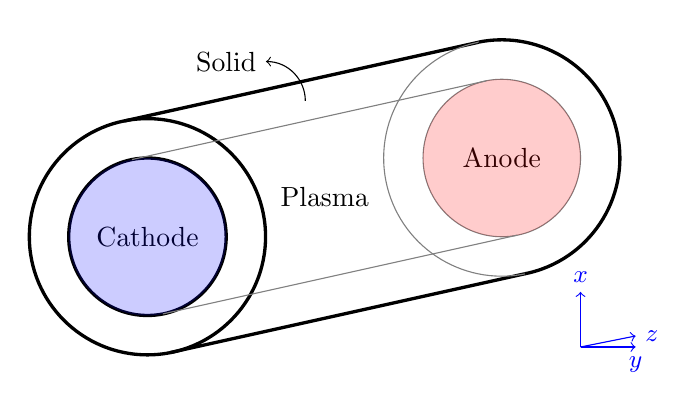
\begin{tikzpicture}
    \coordinate (O1) at (0,0);
    \draw[very thick] (O1) circle (1) node {Cathode};
    \fill[blue, opacity=0.2] (O1) circle (1);
    \draw[very thick] (O1) circle (1.5);
    \coordinate (O2) at (4.5,1) ;
    \draw[gray] (O2) circle (1);
    \node at (O2) {Anode};
    \node at (barycentric cs:O1=1,O2=1) {Plasma}; 
    \fill[red, opacity=0.2] (O2) circle (1);
    \coordinate (S1) at ([shift={(-0.196,0.98)}]O1);
    \coordinate (S2) at ([shift={(-0.196,0.98)}]O2);
    \coordinate (P1) at ([shift={(0.196,-0.98)}]O1);
    \coordinate (P2) at ([shift={(0.196,-0.98)}]O2);
    \draw[gray] (S1) -- (S2);
    \draw[gray] (P1) -- (P2);
    \coordinate (SS1) at ([shift={({-0.196*1.5},{0.98*1.5})}]O1);
    \coordinate (SS2) at ([shift={({-0.196*1.5},{0.98*1.5})}]O2);
    \coordinate (PP1) at ([shift={({0.196*1.5},{-0.98*1.5})}]O1);
    \coordinate (PP2) at ([shift={({0.196*1.5},{-0.98*1.5})}]O2);
    \draw[very thick] (SS1) -- (SS2);
    \draw[very thick] (PP1) -- (PP2); 
    \draw[gray] (SS2) arc (101.31:180+101.31:1.5);
    \draw[very thick] (PP2) arc (101.31-180:101.31:1.5);
    \draw[-to] (barycentric cs:SS1=1,SS2=1,S1=1,S2=1) to[out=90,in=0] ([shift={(-0.5,0.5)}]barycentric cs:SS1=1,SS2=1,S1=1,S2=1) node[left] {Solid};
    \begin{scope}[shift={(5.5,-1.4)}]
    \draw[blue, -to] (0,0) -- (0.7,0.14) node[right]{\small $z$};
    \draw[blue, -to] (0,0) -- (0,0.7) node[above]{\small $x$};
    \draw[blue, -to] (0,0) -- (0.7,0) node[below]{\small $y$};
    \end{scope}
    \end{tikzpicture}
    \caption{Sketch of the computational domain of the case in \cite{fuchs_2021}. Different from the one in this thesis (see Fig. \ref{fig:sketch_domain}), there is a solid enclosing sleeve, and the plasma is confined at the inner area.}
    \label{fig:sketch_domain_fusch}
\end{figure}
Consequently, the following Maxwell's equations to be solved in the insulating solid domain
\begin{align}
    \partial_t \mathbf{B} + \nabla \times \mathbf{E} &= 0, \label{equ:tmp__1}\\ 
    \lambda^2 \partial_t \mathbf{E} - \nabla \times \mathbf{B} &= 0,  \label{equ:tmp__3}\\
    \nabla \cdot \mathbf{B} &= 0, \\
    \lambda^2 \nabla \cdot \mathbf{E} &= 0 \label{equ:tmp__2}.
\end{align}
Supplemented by suitable BCs, the problem is well-posed for $\lambda > 0$. Nonetheless, the $\lambda \rightarrow 0$ limit would lose control of the irrotational part of $\mathbf{E}$-field since only the term curl$\mathbf{E}$ remains in the equations when $\lambda = 0$ (equation (\ref{equ:tmp__2}) becomes trivial) and the BCs are not sufficient to uniquely determine an irrotational vector field. 

To circumvent this problem, one can possibly, as \cite{fuchs_2021}, define a small electrical conductivity $\sigma$ for the insulating domain so that Amp\`{e}re's law becomes
\begin{equation*}
    \lambda^2 \partial_t \mathbf{E} - \nabla \times \mathbf{B} = \sigma\mathbf{E},
\end{equation*}
and the $\lambda \rightarrow 0$ limit model regains well-posedness.

The quasi-neutral limit of the Maxwell system in insulating mediums shares much similarity with the eddy current approximation where the propagation speed, namely the light speed, is treated as infinite, and the displacement current $\partial_t\mathbf{D}$ is hence omitted. Recall that in Section \ref{sec:rescaling} we assume $\lambda$ has the same order as $\xi$, the ratio of the typical speed and light speed. Therefore, although the Debye length is not defined in the solid domain where no plasma exists, the $\lambda \rightarrow 0$ limit of the Maxwell system (\ref{equ:tmp__1}) to (\ref{equ:tmp__2}) is supposed to be interpreted as the eddy current approximation. Due to the disappearance of the divergence-free constraint (\ref{equ:tmp__2}) when $\lambda = 0$, the system is not well-posed. This failure might be resolved by enforcing vanishing divergence of the $\mathbf{E}$-field at the $\lambda \rightarrow 0$ limit, which is no longer a consequence of Amp\`{e}re's law (\ref{equ:tmp__3}). In this thesis, we do not pursue this way. One would later see that in the numerical experiments, for simplicity, we cancel the solid domain and extend the plasma domain to the whole domain. Similar to applying a small conductivity, this way recovers the connection between the current density and the $\mathbf{E}$-field.  

\chapter{Numerical Experiments in 1D}
This chapter is devoted to reproducing the results in \cite{degond_2012} upon which our generalized scheme is built. In their work, 1D problems of one-fluid and two-fluid models are treated by FDTD, in the sense that quantities are defined on staggered structured meshes. As is mentioned before, the FDTD method is a subset of the FIT method, and they are equivalent under Cartesian meshes. One can interpret the FIT treatment of 1D problems through the projection of quantities defined on a 3D Cartesian mesh dual onto a 1D axis, as is depicted in Fig. \ref{fig:1d-frame}.

Although Maxwell's equations are inherently 3D, their reduction in 1D can be derived based on some assumptions and, thanks to great simplification on notations and implementations, helps to test numerical schemes. In this chapter, three cases are tested: one-fluid and two-fluid models tested in \cite{degond_2012}, and additionally the two-fluid model with friction terms. The verification is meant to pave the way for testing in the 3D setting.    

\section{One-fluid model}
In the one-fluid model, only the dynamics of electrons are to be simulated while the background ions are fixed with a uniform number density of unity. The ions are singly-charged throughout the thesis if not specifically stated. Since ions are much heavier than electrons, such a model is a reasonable approximation when only the short-term behavior is of interest so that ions have no time to respond. 

The rescaled one-fluid Euler-Maxwell system\footnote{In \cite{degond_2012}, the equation (2.11) is wrong since the mass ratio $\varepsilon^2$ is missing whereas it is necessary to reproduce their results.} is adapted from the general system (\ref{equ:maxwell_faraday_rescaled}) to (\ref{equ:euler_rescaled}) by only keeping one set of fluid equations to describe electrons and setting the number density of ions to be unity:
\begin{align}
    & \partial_t n + \nabla\cdot(n \mathbf{u}) = 0, \label{equ:EM_1f_n}\\
    \varepsilon^2[& \partial_t (n \mathbf{u}) + \nabla \cdot (n \mathbf{u} \otimes \mathbf{u})] + \nabla p(n) = -n(\mathbf{E} + \mathbf{u} \times \mathbf{B}), \label{equ:EM_1f_nu}\\
    & \partial_t \mathbf{B} + \nabla \times \mathbf{E} = 0 \label{equ:EM_1f_faraday}. \\
    \lambda^2 & \partial_t \mathbf{E} - \nabla \times \mathbf{B} = n \mathbf{u}, \label{equ:EM_1f_ampere}\\
    & \nabla\cdot \mathbf{B} = 0, \label{equ:EM_1f_gauss_B} \\
    \lambda^2 & \nabla\cdot \mathbf{E} = 1 - n \label{equ:EM_1f_gauss_E}.
\end{align}
where $n$ and $\mathbf{u}$ stands for electron number density and velocity, $\varepsilon^2$ now stands for electron-ion mass ratio $m_e/m_i$ which is taken to be $10^{-4}$ here. Note that the energy equation is removed by assuming adiabatic process, and the equation of state $p(n) = n^\gamma$ with $\gamma = 5/3$ is supplemented.  

\subsection{Governing equations in 1D} \label{sec:1f-eqs-1d}
The 3D problem is projected onto the 1D axis by assuming vanishing traverse derivatives (see Fig. \ref{fig:1d-frame} for the definition of reference frame). Besides, $u_y, E_y, B_x, B_z$ are set zero for simplicity, which amounts to considering the TE mode. The collision between particles is omitted for the time being. 
\begin{figure}
    \centering
    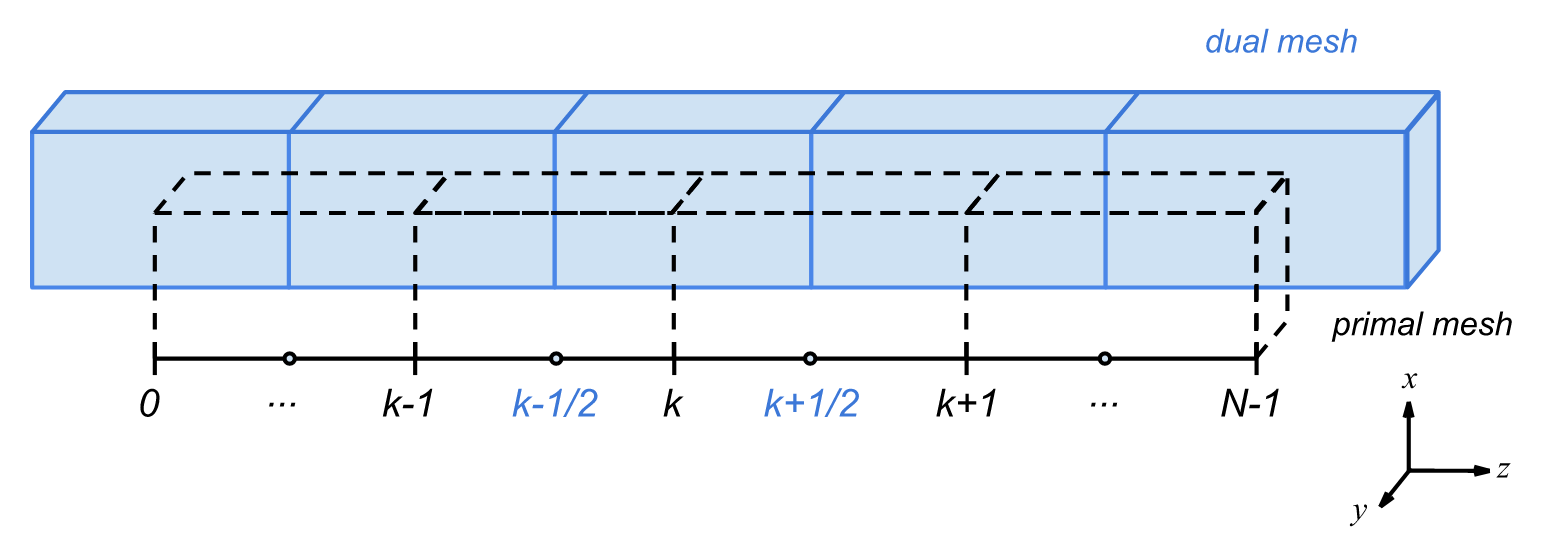
\includegraphics[scale=0.2]{1d_frame.png}
    \caption{Projection of the 3D model onto $z$-axis. Let us consider a Cartesian mesh doublet. The reduction is accomplished by assigning the quantities defined on each cross-section, which is parallel to the $x$-$y$ plane, to its intersection point at $z$-axis. Since it is assumed that no variations occur in each cross-section, the quantities in 3D can be compressed by the ones that locate at each mesh point on the $z$-axis.}
    \label{fig:1d-frame}
\end{figure}

Take all the traverse derivatives $\partial_x, \partial_y$ and $u_y, E_y, B_x, B_z$ to be zero, we get the one-fluid Euler-Maxwell system in 1D:
\begin{align*}
    \partial_t n + \partial_z(nu_z) &= 0, \\
    \varepsilon^2[\partial_t(nu_x) + \partial_z(nu_zu_x)] &= - n(E_x - u_zB_y), \\
    \varepsilon^2[\partial_t(nu_z) + \partial_z(nu_z^2)] + \partial_z(p(n)) &= -n(E_z + u_xB_y), \\
    \partial_t B_y + \partial_z E_x &= 0, \\
    \lambda^2 \partial_t E_x + \partial_z B_y &= nu_x, \\
    \lambda^2 \partial_t E_z &= nu_z, \\
    \lambda^2 \partial_z E_z &= 1 - n,
\end{align*}
as well as the quasi-neutral limit by taking $\lambda \rightarrow 0$:
\begin{align*}
    n &= 1\\
    \varepsilon^2 \partial_t(u_x) &= - E_x, \\
    E_z + u_xB_y &= 0, \\
    u_z &= 0 \\
    \partial_t B_y + \partial_z E_x &= 0, \\
    \partial_z B_y &= nu_x
\end{align*}

\subsection{Full discretization} \label{sec:1f1d-discretization}
Adapt the AP scheme (\ref{equ:maxwell_faraday_ap}) to (\ref{equ:euler_ap}) to this case, and we end up with
\begin{align}
    \frac{n^{m+1}_k - n^m_k}{\delta^m} + \frac{\textcolor{blue}{f^{m+1/2}_{n,k+1/2} - f^{m+1/2}_{n,k-1/2}}}{h} &= 0, \label{equ:1f1d-n}\\
    \frac{(nu_x)^{m+1}_k - (nu_x)^m_k}{\delta^m} + \frac{f^{m}_{u_x,k+1/2} - f^{m}_{u_x,k-1/2}}{h} &= -\frac{n^m_k \textcolor{blue}{E^{m+1}_{x,k}}}{\varepsilon^2} + \frac{n^m_k u^m_{z,k}\Tilde{B}^m_{y,k}}{\varepsilon^2}, \label{equ:1f1d-nux}\\
    \frac{(nu_z)^{m+1}_k - (nu_z)^m_k}{\delta^m} + \frac{f^{m}_{u_z,k+1/2} - f^{m}_{u_z,k-1/2}}{h} &= - \frac{n^m_k \textcolor{blue}{\Tilde{E}^{m+1}_{z,k}}}{\varepsilon^2} - \frac{n^m_k u^m_{x,k}\Tilde{B}^m_{y,k}}{\varepsilon^2}, \label{equ:1f1d-nuz}\\ 
    \frac{B^{m+1}_{y,k+1/2} - B^{m}_{y,k+1/2}}{\delta^m} + \frac{\textcolor{blue}{E^{m+1}_{x,k+1} - E^{m+1}_{x,k}}}{h} &= 0, \label{equ:1f1d-By}\\
    \lambda^2 \frac{E^{m+1}_{x,k} - E^{m}_{x,k}}{\delta^m} + \frac{\textcolor{blue}{B^{m+1}_{y,k+1/2} - B^{m+1}_{y,k-1/2}}}{h} &= \textcolor{blue}{(nu_x)^{m+1}_k}, \label{equ:1f1d-Ex}\\
    \lambda^2 \frac{E^{m+1}_{z,k+1/2} - E^{m}_{z,k+1/2}}{\delta^m} &= \textcolor{blue}{f^{m+1}_{n,k+1/2}}, \label{equ:1f1d-Ez}
\end{align}
where 
\begin{equation*}
    \Tilde{E}^m_{z,k} = \frac{1}{2}(E^m_{z,k+1/2} + E^m_{z,k-1/2}), \ \ \ \Tilde{B}^m_{y,k} = \frac{1}{2}(B^m_{y,k+1/2} + B^m_{y,k-1/2}),
\end{equation*}
is the consequence of interpolation of electromagnetic field, 
and the fluxes read
\begin{align*}
    f^{m+1/2}_{n,k+1/2} & = \frac{1}{2}[\textcolor{blue}{(nu_z)^{m+1}_k + (nu_z)^{m+1}_{k+1}} + \mu^m_{k+1/2}(n^m_k - n^m_{k+1})], \\
    f^{m}_{u_x,k+1/2} & = \frac{1}{2}[(nu_zu_x)^{m}_k + (nu_zu_x)^{m}_{k+1} + \mu^m_{k+1/2}((nu_x)^m_k - (nu_x)^m_{k+1})], \\
    f^{m}_{u_z,k+1/2} & = \frac{1}{2}[(nu_z^2 + p(n)/\varepsilon^2)^{m}_k + (nu_z^2 + p(n)/\varepsilon^2)^{m}_{k+1} + \mu^m_{k+1/2}((nu_z)^m_k - (nu_z)^m_{k+1})]. \\
\end{align*}

\subsection{Numerical results}
A Riemann problem, namely a discontinuous initial condition with two states, is considered. The spatial domain is $[-0.1, 0.1]$. Initially, 
\begin{align*}
    & n(z,0) = 1,\ \ u_z(z,0) = \chi_{[-0.1,0]}(z) - \chi_{[0,0.1]}(z), \\
    & u_x(z,0) = B_y(z,0) = E_x(z,0) = E_z(z,0) = 0.
\end{align*}
Homogeneous Neumann boundary condition is enforced for all the variables for simplicity whereas more sophisticate BC\footnote{In \cite{degond_2012}, Silver-M\"{u}ller condition is used.} is employed in \cite{degond_2012}. The experiments show that no distinct difference occurs. 

To verify the implementation, a grid convergence study is done, see Fig. \ref{fig:grid_study_1d1f}. Due to the discontinuity of solutions, the expected convergence rate for $L^1$-norm error is $1/2$. Since no analytic solution is available, the reference solution is obtained using very fine mesh ($N = 16385$). In addition, the convergence of the number density and the $z$-momentum as the underlying mesh being refined is displayed in Fig. \ref{fig:grid_study_field_1d1f} for $\lambda = 0.01$. Conformity with the results in \cite{degond_2012} is demonstrated by Fig. \ref{fig:lambdas_1d1f} and \ref{fig:lambdas_ref_1d1f}. For $\lambda = 1$, the coupling of fluid motions and electromagnetic fields is weak so that the solution behaves like a shock tube. With decreasing $\lambda$, the coupling effect becomes noticeable. For $\lambda \ll 1$, the solutions converge to quasi-neutral limit. The performance of the scheme when $\lambda = 0$ is also shown in Fig. \ref{fig:lambdas_1d1f}, which leads to a valid solution and nicely reproduces the theoretical solution ($n = 1$ and $u_z = 0$). Slight difference happens for the $z$-momentum when $\lambda = 10^{-4}$, which might result from the different treatment of BC. 

\begin{figure}
    \centering
    \includegraphics{grid_study_1d1f.eps}
    \caption{Grid convergence study for solutions for $\lambda = 10^{-2}$ at $T = 0.0003$. The reference solution is generated by simulation with $N = 16385$. The rate of convergence is roughly 0.5.}
    \label{fig:grid_study_1d1f}
\end{figure}
\begin{figure}
    \centering
    \includegraphics{grid_study_field_1d1f.eps}
    \caption{Comparison of solutions generated by meshes of different sizes. The solutions are computed for $\lambda = 0.01$ at $t=0.0005$.}
    \label{fig:grid_study_field_1d1f}
\end{figure}
\begin{figure}
    \centering
    \includegraphics[scale=1]{lambdas_1d1f.eps}
    \caption{1D one-fluid case of $\lambda = 1, 10^{-2}, 10^{-4}, 0$ at $t = 0.0005$ with $N = 10^3$.}
    \label{fig:lambdas_1d1f}
\end{figure}
\begin{figure}
    \centering
    \includegraphics[scale=0.4]{lambdas_ref_1d1f.png}
    \caption{Results of \cite{degond_2012} at $T = 0.0005$ with $N = 10^3$. }
    \label{fig:lambdas_ref_1d1f}
\end{figure}

\section{Two-fluid model} \label{sec:two_fluid_model}
\subsection{Governing equations in 1D} \label{sec:1d_two_fluid_equations}
Compared to one-fluid model, in two-fluid model the motion of ions is taken into account through one more set of fluid equations. The rescaled two-fluid Euler-Maxwell system reads
\begin{align*}
    \partial_t n_i + \nabla\cdot(n_i \mathbf{u}_i) &= 0, \\
    \partial_t (n_i \mathbf{u}_i) + \nabla \cdot (n_i \mathbf{u}_i \otimes \mathbf{u}_i) + \nabla p(n_i) &= n_i(\mathbf{E} + \mathbf{u}_i \times \mathbf{B}),\\
    \partial_t n_e + \nabla\cdot(n_e \mathbf{u}_e) &= 0, \\
    \varepsilon^2[\partial_t (n_e \mathbf{u}_e) + \nabla \cdot (n_e \mathbf{u}_e \otimes \mathbf{u}_e)] + \nabla p(n_e) &= -n_e(\mathbf{E} + \mathbf{u}_e \times \mathbf{B}),\\
    \partial_t \mathbf{B} + \nabla \times \mathbf{E} &= 0. \\
    \lambda^2 \partial_t\mathbf{E} - \nabla \times \mathbf{B} &= -(n_i \mathbf{u}_i - n_e \mathbf{u}_e),\\
    \nabla\cdot \mathbf{B} &= 0, \\
    \lambda^2 \nabla\cdot \mathbf{E} &= n_i - n_e,
\end{align*}

Following the same assumption as Section \ref{sec:1f-eqs-1d} and supplementing the mass and momentum equations for ions, we obtain the two-fluid Euler-Maxwell system in 1D:
\begin{align*}
    \partial_t n_i + \partial_z(n_i u_{iz}) &= 0, \\
    \partial_t(n_i u_{ix}) + \partial_z(n_i u_{iz} u_{ix}) &= n_i(E_x - u_{iz} B_y), \\
    \partial_t(n_i u_{iz}) + \partial_z(n_i u_{iz}^2 + P(n_i)) &= n_i(E_z + u_{ix} B_y), \\
    \partial_t n_e + \partial_z(n_e u_{ez}) &= 0, \\
    \varepsilon^2 [ \partial_t(n_e u_{ex}) + \partial_z(n_e u_{ez} u_{ex}) ] &= - n_e(E_x - u_{ez} B_y), \\
    \varepsilon^2 [ \partial_t(n_e u_{ez}) + \partial_z(n_e u_{ez}^2) ] + \partial_z(P(n_e)) &= -n_e(E_z + u_{ex} B_y), \\
    \partial_t B_y + \partial_z E_x &= 0, \\
    \lambda^2 \partial_t E_x + \partial_z B_y &= n_e u_{ex} - n_i u_{ix}, \\
    \lambda^2 \partial_t E_z &= n_e u_{ez} - n_i u_{iz}, \\
    \lambda^2 \partial_z E_z &= n_i - n_e,
\end{align*}
where the subscript $i$ and $e$ represent ion and electron variables respectively.

The discretization follows the same principle as illustrated in Section \ref{sec:1f1d-discretization} and thus is omitted here.

\subsection{Numerical results} \label{sec:1d_two_fluid_numerical_results}
The same case as the previous one is tested here. The initial condition remains unchanged for electron variables and electromagnetic fields. Additionally, for ion variables, we set
\begin{align*}
    n_i(z,0) = 1, \ \ u_{ix}(z,0) = u_{iz}(z,0) = 0, 
\end{align*}
namely, the ion is uniform and at rest at the initial time.
\begin{figure}
    \centering
    \includegraphics{grid_study_field_1d2f.eps}
    \caption{Comparison of solutions generated by meshes of different sizes. The solutions are computed for $\lambda = 0.01$ at $t = 5 \times 10^{-4}$.}
    \label{fig:grid_study_field_1d2f}
\end{figure}
\begin{figure}
    \centering
    \includegraphics[scale=1]{lambdas_1d2f.eps}
    \caption{1D two-fluid case of $\lambda = 1, 10^{-2}, 10^{-4}, 0$ at $t = 5\times10^{-4}$ with $N = 10^3$.}
    \label{fig:lambdas_1d2f}
\end{figure}
\begin{figure}
    \centering
    \includegraphics[scale=0.45]{lambdas_ref_1d2f_1.png}
    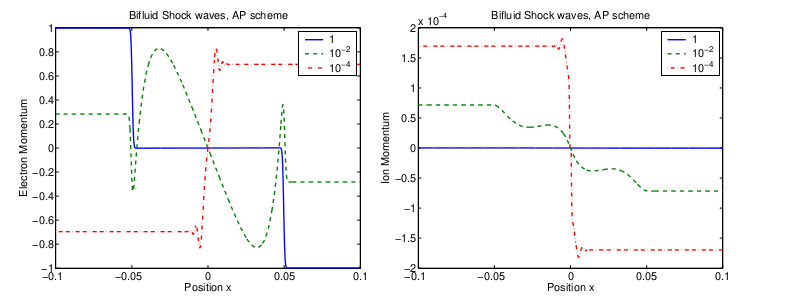
\includegraphics[scale=0.45]{lambdas_ref_1d2f_2.png}
    \caption{Results of \cite{degond_2012} at $t = 5\times10^{-4}$ with $N = 10^3$.}
    \label{fig:lambdas_ref_1d2f}
\end{figure}


For the sake of verification, the convergence of certain quantities as the mesh being refined is demonstrated in Fig. \ref{fig:grid_study_field_1d2f} for $\lambda = 0.01$. Results of the same resolution ($N = 10^4$) with different $\lambda$ are shown in Fig. \ref{fig:lambdas_1d2f}. As reference, results in \cite{degond_2012} are shown in Fig. \ref{fig:lambdas_ref_1d2f}. They almost\footnote{Obviously, electron momentum when $\lambda = 10^{-4}$ in Fig. \ref{fig:lambdas_ref_1d2f} is incorrect since electron and ion momentum are supposed to be equal in quasi-neutral limit} coincide. Besides, the case corresponding to $\lambda = 0$ provided in Fig. \ref{fig:lambdas_1d2f} shows consistency with the quasi-neutral condition $n_i = n_e$ and $n_eu_{ez} = n_iu_{iz}$.

\section{Two-fluid model with collision term} \label{sec:1d2f_coll}
\subsection{Governing equations}
As one step further towards a more realistic model, we take into account the collision between electrons and ions by including the friction term (\ref{equ:collision_rescaled}). The inclusion of collision term leads to the equations
\begin{align*}
    \partial_t n_i + \nabla\cdot(n_i \mathbf{u}_i) &= 0, \\
    \partial_t (n_i \mathbf{u}_i) + \nabla \cdot (n_i \mathbf{u}_i \otimes \mathbf{u}_i) + \nabla p(n_i) &= n_i(\mathbf{E} + \mathbf{u}_i \times \mathbf{B}) + \colorbox{orange!20}{$\alpha^\text{coll} n_en_i(\mathbf{u}_i - \mathbf{u}_e)$},\\
    \partial_t n_e + \nabla\cdot(n_e \mathbf{u}_e) &= 0, \\
    \varepsilon^2[\partial_t (n_e \mathbf{u}_e) + \nabla \cdot (n_e \mathbf{u}_e \otimes \mathbf{u}_e)] + \nabla p(n_e) &= -n_e(\mathbf{E} + \mathbf{u}_e \times \mathbf{B}) + \colorbox{orange!20}{$\alpha^\text{coll}  n_en_i(\mathbf{u}_e - \mathbf{u}_i)$},\\
    \partial_t \mathbf{B} + \nabla \times \mathbf{E} &= 0. \\
    \lambda^2 \partial_t\mathbf{E} - \nabla \times \mathbf{B} &= -(n_i \mathbf{u}_i - n_e \mathbf{u}_e),\\
    \nabla\cdot \mathbf{B} &= 0, \\
    \lambda^2 \nabla\cdot \mathbf{E} &= n_i - n_e,
\end{align*}
where $\alpha^\text{coll}$ is the dimensionless prefactor and we treat it as a pre-defined parameter.

In our 1D setting, the governing equations become
\begin{align*}
    \partial_t n_i + \partial_z(n_i u_{iz}) &= 0, \\
    \partial_t(n_i u_{ix}) + \partial_z(n_i u_{iz} u_{ix}) &= n_i(E_x - u_{iz} B_y) + \colorbox{orange!20}{$\alpha^\text{coll} n_e n_i (u_{ex} - u_{ix})$}, \\
    \partial_t(n_i u_{iz}) + \partial_z(n_i u_{iz}^2 + P(n_i)) &= n_i(E_z + u_{ix} B_y) + \colorbox{orange!20}{$\alpha^\text{coll} n_e n_i (u_{ez} - u_{iz})$}, \\
    \partial_t n_e + \partial_z(n_e u_{ez}) &= 0, \\
    \varepsilon^2 [ \partial_t(n_e u_{ex}) + \partial_z(n_e u_{ez} u_{ex}) ] &= - n_e(E_x - u_{ez} B_y) + \colorbox{orange!20}{$\alpha^\text{coll} n_e n_i (u_{ix} - u_{ex})$}, \\
    \varepsilon^2 [ \partial_t(n_e u_{ez}) + \partial_z(n_e u_{ez}^2) ] + \partial_z(P(n_e)) &= -n_e(E_z + u_{ex} B_y) + \colorbox{orange!20}{$\alpha^\text{coll} n_e n_i (u_{iz} - u_{ez})$}, \\
    \partial_t B_y + \partial_z E_x &= 0, \\
    \lambda^2 \partial_t E_x + \partial_z B_y &= n_e u_{ex} - n_i u_{ix}, \\
    \lambda^2 \partial_t E_z &= n_e u_{ez} - n_i u_{iz}, \\
    \lambda^2 \partial_z E_z &= n_i - n_e.
\end{align*}

\subsection{Full discretization}
The full discretization is merely the one used in the previous section plus implicit collision terms. The implicitness is owing to the stiffness incurred from the potentially large value of $\varepsilon^{-2}\alpha^\text{coll}$.
\begin{align*}
    \frac{n^{m+1}_{i,k} - n^m_{i,k}}{\delta^m} + \frac{\textcolor{blue}{f^{m+1/2}_{n_i,k+1/2} - f^{m+1/2}_{n_i,k-1/2}}}{h} &= 0, \\
    \frac{(n_iu_{ix})^{m+1}_k - (n_iu_{ix})^m_k}{\delta^m} + \frac{f^{m}_{u_{ix},k+1/2} - f^{m}_{u_{ix},k-1/2}}{h} &= n^m_{i,k}( \textcolor{blue}{E^{m+1}_{x,k}} - u^m_{iz,k}\Tilde{B}^m_{y,k}) \\
    & + \colorbox{orange!20}{$\alpha^\text{coll} \left[n^m_{i,k}\textcolor{blue}{(n_eu_{ex})^{m+1}_k} - n^m_{e,k}\textcolor{blue}{(n_iu_{ix})^{m+1}_k}\right]$},\\
    \frac{(n_iu_{iz})^{m+1}_k - (n_iu_{iz})^m_k}{\delta^m} + \frac{f^{m}_{u_{iz},k+1/2} - f^{m}_{u_{iz},k-1/2}}{h} &= n^m_{i,k}(\textcolor{blue}{\Tilde{E}^{m+1}_{z,k}} + u^m_{ix,k}\Tilde{B}^m_{y,k}) \\
    & + \colorbox{orange!20}{$\alpha^\text{coll} \left[n^m_{i,k}\textcolor{blue}{(n_eu_{ez})^{m+1}_k} - n^m_{e,k}\textcolor{blue}{(n_iu_{iz})^{m+1}_k}\right]$},\\
    \frac{n^{m+1}_{e,k} - n^m_{e,k}}{\delta^m} + \frac{\textcolor{blue}{f^{m+1/2}_{n_e,k+1/2} - f^{m+1/2}_{n_e,k-1/2}}}{h} &= 0,  \\
    \varepsilon^2\frac{(n_eu_{ex})^{m+1}_k - (n_eu_{ex})^m_k}{\delta^m} + \frac{f^{m}_{u_{ex},k+1/2} - f^{m}_{u_{ex},k-1/2}}{h} &= - n^m_{e,k}( \textcolor{blue}{E^{m+1}_{x,k}} - u^m_{ez,k}\Tilde{B}^m_{y,k}) \\
    & - \colorbox{orange!20}{$\alpha^\text{coll} \left[n^m_{i,k}\textcolor{blue}{(n_eu_{ex})^{m+1}_k} - n^m_{e,k}\textcolor{blue}{(n_iu_{ix})^{m+1}_k}\right]$},\\
    \varepsilon^2\frac{(n_eu_{ez})^{m+1}_k - (n_eu_{ez})^m_k}{\delta^m} + \frac{f^{m}_{u_{ez},k+1/2} - f^{m}_{u_{ez},k-1/2}}{h} &= - n^m_{e,k}(\textcolor{blue}{\Tilde{E}^{m+1}_{z,k}} + u^m_{ix,k}\Tilde{B}^m_{y,k}) \\
    & - \colorbox{orange!20}{$\alpha^\text{coll} \left[n^m_{i,k}\textcolor{blue}{(n_eu_{ez})^{m+1}_k} - n^m_{e,k}\textcolor{blue}{(n_iu_{iz})^{m+1}_k}\right]$},\\    
    \frac{B^{m+1}_{y,k+1/2} - B^{m}_{y,k+1/2}}{\delta^m} + \frac{\textcolor{blue}{E^{m+1}_{x,k+1} - E^{m+1}_{x,k}}}{h} &= 0, \\
    \lambda^2 \frac{E^{m+1}_{x,k} - E^{m}_{x,k}}{\delta^m} + \frac{\textcolor{blue}{B^{m+1}_{y,k+1/2} - B^{m+1}_{y,k-1/2}}}{h} &= \textcolor{blue}{(n_eu_{ex})^{m+1}_k - (n_iu_{ix})^{m+1}_k}, \\
    \lambda^2 \frac{E^{m+1}_{z,k+1/2} - E^{m}_{z,k+1/2}}{\delta^m} &= \textcolor{blue}{f^{m+1}_{n_e,k+1/2} - f^{m+1}_{n_i,k+1/2}}. \\
\end{align*}

\subsection{Numerical results}
We set the friction coefficient $\alpha^\text{coll} = 644$, and stick to the previous initial condition
\begin{align*}
    & n_e(z,0) = n_i(z,0) = 1,\\
    & u_{ez}(z,0) = u_{iz}(z,0) = \chi_{[-0.1,0]}(z) - \chi_{[0,0.1]}(z), \\
    & u_{ex}(z,0) = u_{ix}(z,0) = B_y(z,0) = E_x(z,0) = E_z(z,0) = 0.
\end{align*}
The case with a cell number $N = 1000$ and terminal time $t_{\text{end}} = 0.02$ is tested for $\lambda = 1, 10^{-2}, 10^{-4}, 0$. The number densities and momenta of ions and electrons are shown in Fig. \ref{fig:lambdas_1d2fc}.
\begin{figure}
    \centering
    \includegraphics{lambdas_1d2fc_const.eps}
    \caption{1D two-fluid case with friction terms. Results for $\lambda = 1, 10^{-2}, 10^{-4}, 0$ at $t = 0.02$ with $N = 1000$.}
    \label{fig:lambdas_1d2fc}
\end{figure}
\begin{figure}
    \centering
    \includegraphics{grid_study_field_1d2fc.eps}
    \caption{Comparison of solutions generated by meshes of different sizes. The solutions are computed for $\lambda = 10^{-4}$ at $t = 0.02$.}
    \label{fig:grid_study_field_1d2fc}
\end{figure}
With decreasing $\lambda$, as expected, the densities and $z$-momenta of ion and electron gradually approach each other. However, when $\lambda = 10^{-4}$, spurious spikes exist at the discontinuity of electron momentum field and can be diminished by refining the mesh, as is shown in Fig. \ref{fig:grid_study_field_1d2fc} which also manifests the convergence with respect to the mesh refinement.
\section{Summary}
We have verified the AP scheme proposed in \cite{degond_2012} by reproducing the numerical solutions of one-fluid and two-fluid Euler-Maxwell systems in 1D. Besides, it is also ensured that the inclusion of friction term does not undermine the AP property. To summarize, the scheme works uniformly for $\lambda \in [0,1]$ in the sense that no instability occurs and the transition of different regimes is smooth. Within expect, the quasi-neutral condition $n_i = n_e$ is observed for the limiting case.

In the sequel, the performance of the AP scheme on problems in 3D is to be checked. It expects to pose more challenges due to the boundary treatment in FIT and the inherently more complex 3D structures of Maxwell's equations.

\chapter{Numerical Experiments in 3D} \label{chap:numerical_experiments_in_3d}

In the previous chapter, we have gone through problems in a 1D setting, and have conveyed the basic idea of simulating plasma by AP schemes. As Maxwell's equations are inherently 3D, doing simulations in 3D is essential to gain realistic results. 

We test the AP scheme on a case that is adapted\footnote{Keeping the geometry and BCs being unchanged, we remove the enclosing solid dielectric domain such that the plasma domain coincides with the electromagnetic domain. The reason is illustrated in Section \ref{sec:impact_insulating_domain}.} from the one used in \cite[][chap. 1 sec. 4]{fuchs_2021}---a cylindrical tube filled with plasmas and applied external potentials on both ends. 

In this chapter, a description of the problem is first given, including the domain geometry and boundary conditions. Considerable words are devoted to the enforcement of BCs as well as their well-posedness from an algebraic perspective. Afterward, we elaborate on the procedure of time-stepping, especially the assembling of the linear system. The validity of such a linear system over arbitrary $\lambda$ is critical for attaining the AP property. 

Instead of directly cutting to the fully-coupled system, we first test the behavior of the scheme on the subsystems of the Euler-Maxwell system as verification. Finally, we present the numerical results of the fully-coupled Euler-Maxwell system, on which the AP property is to be verified.

\section{Problem description and mesh generation} \label{sec:problem_description}
The problem setting is a cylindrical domain filled with plasma fluids, and with two electrodes on each end, as is sketched in Fig. \ref{fig:sketch_domain}. From the viewpoint of the Euler system, the cylinder is enclosed by a non-penetrating wall whereas the plasma fluids are allowed to inflow and outflow through the electrode surfaces. Regarding the Maxwell system, external electric potentials are applied on the electrodes, and the enclosing boundary is considered insulating. 

Under such a setting, the motions of charged particles of the plasma are driven by the external potential, giving rise to an electromagnetic field, which in turn exerts Lorentz force on the charged particles. This setting is intended for simulating electric arcs.

We discretize the spatial domain by an unstructured mesh doublet ($\mathcal{M}, \Tilde{\mathcal{M}}$) which consists of prisms aligned with the axial direction. The mesh generation is realized by the code developed in \cite{fuchs_2021}. The detailed algorithm is omitted. In principle, a circle is first discretized with a 2D mesh which afterward is extended along the axial direction to form the 3D mesh. Based on the generated primal mesh, a dual mesh conforming to the duality requirements, as is illustrated in Section \ref{sec:mesh_duality}, can be constructed with additional attention on the cut-off boundary that is discussed in Section \ref{sec:boundary_treatment}. An example of the primal and dual meshes is shown in Fig. \ref{fig:primal_dual_meshes}.

\begin{figure}
    \centering
    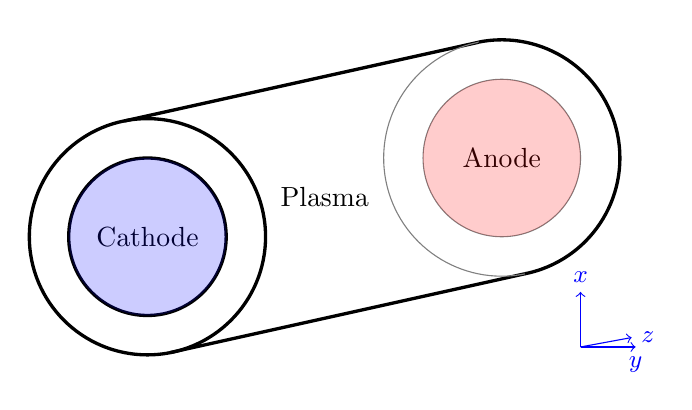
\begin{tikzpicture}
    \coordinate (O1) at (0,0);
    \draw[very thick] (O1) circle (1) node {Cathode};
    \fill[blue, opacity=0.2] (O1) circle (1);
    \draw[very thick] (O1) circle (1.5);
    \coordinate (O2) at (4.5,1) ;
    \draw[gray] (O2) circle (1);
    \node at (O2) {Anode};
    \node at (barycentric cs:O1=1,O2=1) {Plasma}; 
    \fill[red, opacity=0.2] (O2) circle (1);
    \coordinate (S1) at ([shift={(-0.196,0.98)}]O1);
    \coordinate (S2) at ([shift={(-0.196,0.98)}]O2);
    \coordinate (P1) at ([shift={(0.196,-0.98)}]O1);
    \coordinate (P2) at ([shift={(0.196,-0.98)}]O2);
    \coordinate (SS1) at ([shift={({-0.196*1.5},{0.98*1.5})}]O1);
    \coordinate (SS2) at ([shift={({-0.196*1.5},{0.98*1.5})}]O2);
    \coordinate (PP1) at ([shift={({0.196*1.5},{-0.98*1.5})}]O1);
    \coordinate (PP2) at ([shift={({0.196*1.5},{-0.98*1.5})}]O2);
    \draw[very thick] (SS1) -- (SS2);
    \draw[very thick] (PP1) -- (PP2); 
    \draw[gray] (SS2) arc (101.31:180+101.31:1.5);
    \draw[very thick] (PP2) arc (101.31-180:101.31:1.5);
    \begin{scope}[shift={(5.5,-1.4)}]
    \draw[blue, -to] (0,0) -- (0.65,0.12) node[right]{\small $z$};
    \draw[blue, -to] (0,0) -- (0,0.7) node[above]{\small $x$};
    \draw[blue, -to] (0,0) -- (0.7,0) node[below]{\small $y$};
    \end{scope}
    \end{tikzpicture}
    \caption{Sketch of the computational domain: a cylinder filled with plasma and with two electrodes at the ends.}
    \label{fig:sketch_domain}
\end{figure}

\begin{figure}
    \centering
    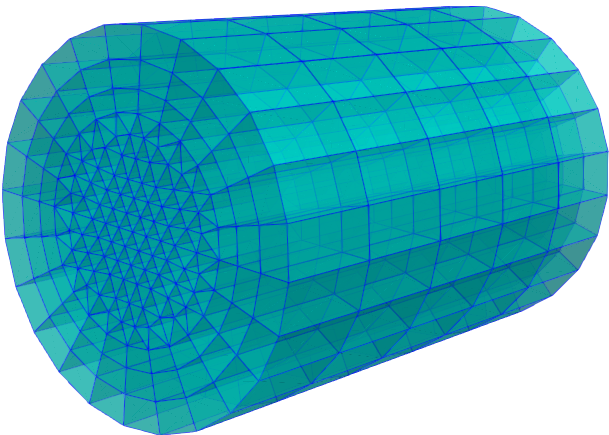
\includegraphics[scale=0.4]{primal_mesh.png}
    \hspace{2cm}
    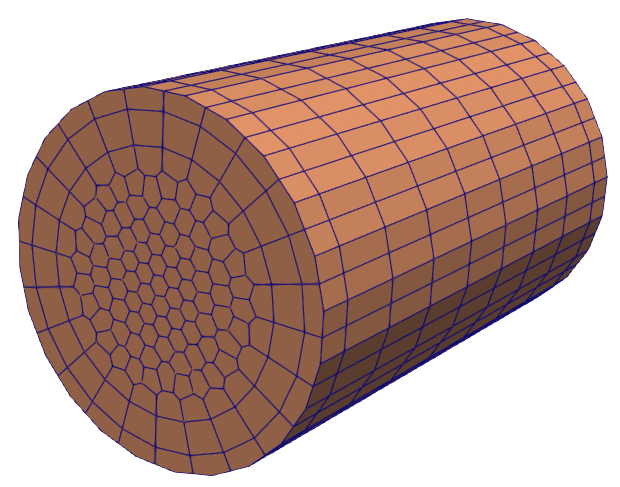
\includegraphics[scale=0.4]{dual_mesh.png}
    \caption{Primal (left) and dual (right) meshes used for the 3D testing case. They are generated by the code developed in \cite{fuchs_2021}.}
    \label{fig:primal_dual_meshes}
\end{figure}

\section{Boundary conditions} \label{sec:numerical_experiement_bc}

\begin{figure}
    \centering
    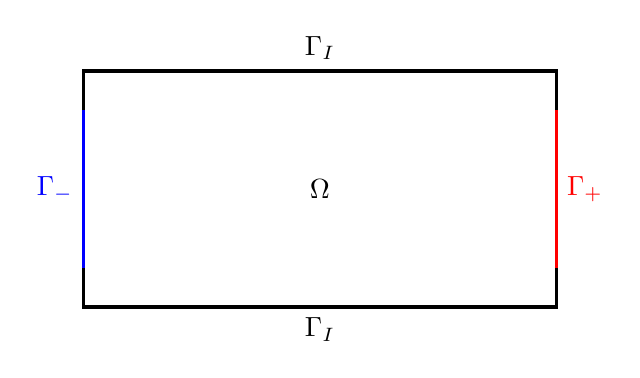
\begin{tikzpicture}
        \coordinate (A1) at (0,1.5);
        \coordinate (A2) at (0,1);
        \coordinate (A3) at (0,-1);
        \coordinate (A4) at (0,-1.5);
        \coordinate (B1) at (6,1.5);
        \coordinate (B2) at (6,1);
        \coordinate (B3) at (6,-1);
        \coordinate (B4) at (6,-1.5);
        \draw[very thick] (A2) -- (A1) -- node[above]{$\Gamma_I$} (B1) -- (B2);
        \draw[very thick] (A3) -- (A4) -- node[below]{$\Gamma_I$} (B4) -- (B3);
        \draw[very thick, blue] (A2) -- node[left]  {$\Gamma_-$}  (A3);
        \draw[very thick, red]  (B2) -- node[right] {$\Gamma_+$}  (B3);
        \node at (3,0) {$\Omega$};
    \end{tikzpicture}
    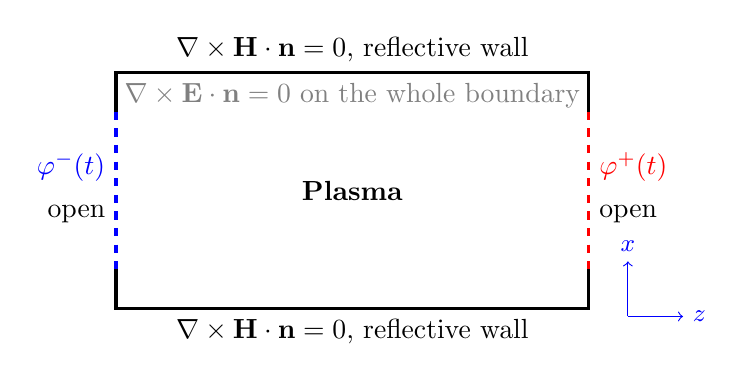
\begin{tikzpicture}
        \coordinate (A1) at (0,1.5);
        \coordinate (A2) at (0,1);
        \coordinate (A3) at (0,-1);
        \coordinate (A4) at (0,-1.5);
        \coordinate (B1) at (6,1.5);
        \coordinate (B2) at (6,1);
        \coordinate (B3) at (6,-1);
        \coordinate (B4) at (6,-1.5);
        \draw[very thick] (A2) -- (A1) -- node[above]{$\nabla \times \mathbf{H}\cdot \mathbf{n} = 0$, reflective wall}  node[below, gray]{$\nabla \times \mathbf{E} \cdot \mathbf{n} = 0$ on the whole boundary} (B1) -- (B2);
        \draw[very thick] (A3) -- (A4) -- node[below]{$\nabla \times \mathbf{H}\cdot \mathbf{n} = 0$, reflective wall} (B4) -- (B3);
        \draw[very thick, dashed, blue] (A2) -- node[left, yshift=0.3cm] {$\varphi^-(t)$} node[left, yshift=-0.3cm] {\textcolor{black}{open}} (A3);
        \draw[very thick, dashed, red]  (B2) -- node[right, yshift=0.3cm]  {$\varphi^+(t)$} node[right, yshift=-0.3cm] {\textcolor{black}{open}}  (B3);
        \node at (3,0) {\textbf{Plasma}};
        \begin{scope}[shift={(6.5,-1.6)}]
        \draw[blue, -to] (0,0) -- (0,0.7) node[above]{\small $x$};
        \draw[blue, -to] (0,0) -- (0.7,0) node[right]{\small $z$};
        \end{scope}
    \end{tikzpicture}
    \caption{Illustration of the boundary conditions: (left) notation of each part of the boundary; (right) boundary conditions at each part of the boundary.}
    \label{fig:bc}
\end{figure}

Before presenting the BCs, we notate the different parts of the computational domain. The whole domain is $\Omega \subset \mathbb{R}^3$ consisting of the interior $\Omega^\circ$ and boundary $\partial \Omega := \Gamma$. The cathode and anode are modeled by a 2D surface without thickness and thus lie on the boundary. They are notated $\Gamma_-$ and $\Gamma_+$ respectively. The rest of the boundary $\Gamma_I := \Gamma \backslash (\Gamma_- \cup \Gamma_+)$ is the insulating boundary. These are visualized in Fig. \ref{fig:bc} (left). 

We would like to stress that the boundary of the plasmas domain, namely the domain where the Euler equations are defined, coincides with the artificial truncation for the electromagnetic field.

For Maxwell's equations, we adopt the so-called \emph{ECE boundary conditions} in the sense that 1) at the electrodes electric potentials $\varphi^-(t)$ and $\varphi^+(t)$ are enforced externally
; 2) the tangential $\mathbf{E}$-field is curl-free on $\Gamma$; 3) the tangential $\mathbf{H}$-field is curl-free at $\Gamma_I$. 

For the Euler system, the wall boundary is considered \emph{reflective} and requires vanishing normal velocity. At $\Gamma_+$ and $\Gamma_-$ where the electrodes lie, we stick to \cite{fuchs_2021}, and employ the \emph{open} BC, allowing the fluids to freely pass in the sense of zero gradients of the fluid quantities. 

Since the electrons and ions cannot penetrate the reflective wall, the orthogonal current vanishes on $\Gamma_I$. By Amp\`{e}re's law (\ref{equ:maxwell_ampere_rescaled}) the insulating BC $\text{curl}\mathbf{H} \cdot \mathbf{n} = 0$ is equivalent to $\mathbf{D}\cdot\mathbf{n} = 0$ provided $\mathbf{D}\cdot\mathbf{n} = 0$ is satisfied at the initial time. To study the asymptotic behavior of the system, the latter one is suitable and thus is actually adopted because of the reason discussed in Section \ref{sec:impact_of_bc}.  

To summarize, 
\begin{align}
    \varphi &= \varphi^-(t)\ \ \text{on} \ \ \Gamma_-, \label{equ:bc_1}\\
    \varphi &= \varphi^+(t)\ \ \text{on} \ \ \Gamma_+, \label{equ:bc_2}\\
    \text{curl} \mathbf{E} \cdot \mathbf{n} &= 0\ \ \text{on} \ \  \Gamma_I,  \label{equ:bc_3}\\
    \text{curl} \mathbf{H} \cdot \mathbf{n} = 0 \Leftrightarrow \mathbf{D} \cdot \mathbf{n} &= 0\ \  \text{on} \ \  \Gamma_I, \label{equ:bc_4}\\
    \mathbf{u_*}\cdot \mathbf{n} &= 0 \ \ \text{on} \ \ \Gamma_I, \label{equ:bc_5}\\
    \text{grad}\mathbf{U_*} \cdot \mathbf{n} &= \mathbf{0} \ \ \text{on} \ \ \Gamma_+\cup\Gamma_-. \label{equ:bc_6}
\end{align}
where $\mathbf{n}$ denotes the outer normal vector. Recall that $\mathbf{u}_*$ and $\mathbf{U}_*$ denotes the velocity and conservative fluid quantities of species $*$. 

To verify that the BCs lead to a well-posed problem, especially for Maxwell's equations\footnote{The BCs for the Euler system are rather classical. See \cite[][Chap. 7]{leveque_2002} for a general introduction, or \cite[][sec. 2e]{mishra_2019b} for the specific implementation for the Euler equations.}, we want to check that these BCs in the discrete level lead to a solvable linear system. A \emph{necessary} condition is that \emph{the number of unknown variables and the number of (independent) algebraic equations coincide}.

We would like to remark that the time-stepping for Euler equations (\ref{equ:euler_ap}) do not involve solving any linear system since the implicit mass term in (\ref{equ:flux_ap}) can be obtained through the momentum equations. As for the implicit term $\mathbf{E}^{m+1}$ in the source term (\ref{equ:rhs_ap}), it is obtained through updating the Maxwell system. Therefore, only the evolution of the Maxwell system entails solving a linear system, whose validity is discussed here.

First, a meticulous classification and counting for facets of meshes are done as follows:
\begin{align*}
    \#\  \text{primal cell}\ \  &N_V \\
    \#\  \text{primal edge}\ \  &N_L := \underbrace{N^+_L + N^-_L + N^I_L}_{N^\partial_L} + N^\circ_L  \\
    \#\  \text{primal face}\ \  &N_A := \underbrace{N_A^+ + N_A^- + N^I_A}_{N^\partial_A} + N^\circ_A  \\
    \#\  \text{primal vertex}\ \  &N_P := \underbrace{N_P^+ + N_P^- + N^I_P}_{N^\partial_P} + N^\circ_P \\
    \#\  \text{dual cell}\ \  &N_{\Tilde{V}} := N_p \\
    \#\  \text{dual edge}\ \  &N_{\Tilde{L}} := \underbrace{N^\partial_{\Tilde{L}}}_{=N^\partial_L} + \underbrace{N^\circ_{\Tilde{L}}}_{=N_A} \\
    \#\  \text{dual face}\ \  &N_{\Tilde{A}} := \underbrace{N^\partial_{\Tilde{A}}}_{=N^\partial_P} + \underbrace{N^\circ_{\Tilde{A}}}_{=N_L}
\end{align*}
where the superscripts indicate the domains to which facets belong to, and $+,-,I,\circ,\partial$ represent $\Gamma_+, \Gamma_-, \Gamma_I, \Omega^\circ, \partial \Omega$ respectively. As is discussed in Section \ref{sec:boundary_treatment}, auxiliary dual facets are needed to trim $\Tilde{\mathcal{M}}$ such that $\mathcal{M}$ and $\Tilde{\mathcal{M}}$ share the same boundary. By inspecting Fig. \ref{fig:illustraion_dual_boundary}, one can realize that the auxiliary dual edges have the same number as the primal boundary edges since they intersect with each other; the auxiliary dual faces have the same number as the primal boundary vertices. These amount to $N^\partial_{\Tilde{L}} = N^\partial_L, N^\partial_{\Tilde{A}} = N^\partial_P$. Note that these number relationships are attained on the premise that non-straight edges and non-flat faces are admissible.

Next, we count the number of unknowns. From the BCs (\ref{equ:bc_1})(\ref{equ:bc_3})  we know that the tangential $\mathbf{E}$-field is irrotational at the whole boundary $\partial\Omega$, which allows a scalar potential function $\varphi$ on $\partial \Omega$ with $\text{grad}_\tau \varphi = \mathbf{E}_\tau$. In the discrete case, $\bm{\varphi}$ is a scalar vector whose entries are defined on each primal vertex on $\partial \Omega$. The collection of boundary electric voltage $\mathbf{e}^\partial$ is retrieved by $\mathbf{e}^\partial = \mathbb{G}_\partial \bm{\varphi}$ where $\mathbb{G}_\partial$ stands for the discrete grad operator on the boundary. Besides, additional dual edges and faces at boundary, to which the integrals of the $\mathbf{H}$-field and the $\mathbf{D}$-field are assigned, give rise to unknown $\mathbf{h^\partial}$ and $\mathbf{d^\partial}$ vectors of sizes $N^\partial_{\Tilde{L}}$ and $N^\partial_{\Tilde{A}}$. The counting of unknown variables is as follows:
\begin{equation*}
    |\mathbf{e}| = N_L, \ \ \ |\mathbf{b}|=N_A, \ \ \ |\mathbf{h}^\partial|=N^\partial_{\Tilde{L}},\ \ \ |\mathbf{d}^\partial| = N^\partial_{\Tilde{A}}, \ \ \ |\bm{\varphi}| = N^\partial_P,
\end{equation*}
where $|\cdot|$ denotes the size of vector. 

Lastly, we collect all the algebraic equations derived from the Maxwell system. The coupling term $\mathbf{j}^{m+1}$ in discrete Ampere's law (\ref{equ:maxwell_ampere_ap}) can be rewritten by electric variables, which will be demonstrated in (\ref{equ:tmp5})(\ref{equ:tmp6}) at the next section. The discrete Faraday's law (\ref{equ:maxwell_faraday_ap}) updates the scalar vector $\mathbf{b}$ which is composed of integrals of $\mathbf{B}$-field on each primal face; the discrete Amp\`{e}re's law (\ref{equ:maxwell_ampere_ap}) updates $\mathbf{d}$ which is composed of integrals of $\mathbf{D}$-field on each dual face; the relation $\mathbf{e}^\partial = \mathbb{G}_\partial \bm{\varphi}$ entails $N^\partial_L$ equations each of which is defined on a boundary primal edge; the entries of $\bm{\varphi}$ that locate on the electrodes are assigned externally; the insulating BC (\ref{equ:bc_4}) needs to be satisfied at each dual face that lies in $\Gamma_I$. In summary, the counting of algebraic equations is as follows:
\begin{align*}
    \text{discrete Faraday law (\ref{equ:maxwell_faraday_ap})} \ \ &\longrightarrow\ \  N_A \ \ \text{equations} \\
    \text{discrete Ampere law (\ref{equ:maxwell_ampere_ap})} \ \ &\longrightarrow\ \  N_{\Tilde{A}} \ \ \text{equations} \\
     \mathbf{E}_\tau = \text{grad}_\tau \varphi \Rightarrow \mathbf{e}^\partial = \mathbb{G}_\partial \bm{\varphi} \ \ &\longrightarrow\ \  N^\partial_L \ \ \text{equations} \\
    \text{enforced potentials}\ \ \varphi^+(t), \varphi^-(t) \ \ &\longrightarrow\ \  N_P^+ + N_P^- \ \ \text{equations} \\
    \text{insulating BC (\ref{equ:bc_4})} \ \ &\longrightarrow\ \  N_{\Tilde{A}}^I = N_P^I \ \ \text{equations}.
\end{align*}
It is straightforward to check that the numbers of unknowns and the equations match. Specifically, 
\begin{align*}
    \#\text{ of unknowns} &= \colorbox{orange!20}{$N_L$} + \colorbox{blue!20}{$N_A$} + \colorbox{gray!20}{$N_{\Tilde{L}}^\partial$} + \colorbox{orange!20}{$N_{\Tilde{A}}^\partial$} + \colorbox{green!20}{$N_P^\partial$}, \\
    \#\text{ of equations} &= \colorbox{blue!20}{$N_A$} + \colorbox{orange!20}{$N_{\Tilde{A}}$} + \colorbox{gray!20}{$N_L^\partial$} + \colorbox{green!20}{$N_P^+ + N_P^- + N_P^I$},
\end{align*}
where the terms with the same color can be equated by applying the counting relations listed above.

However, the matching of numbers of unknowns and equations does not necessarily result in a valid linear system. Inappropriate BCs could cause the singularity of the linear system, as is discussed in Section \ref{sec:impact_of_bc}. 

\section{Procedure of time-stepping}
In this section, we would like to present the concrete strategy to evolve the whole system, namely calculating variables at $t_{m+1}$ given their values at $t_m$. On one hand, the impact of BCs is not considered when presenting the AP scheme (\ref{equ:maxwell_faraday_ap}) to (\ref{equ:current_ap}). On the other hand, a clever and detailed strategy of establishing the linear system at every time step is necessary. 

To avoid any confusion, the definition of the quantities is repeated in Tab. \ref{tab:def_size_var}. For better illustration, matrices used in this section are supplemented with both superscript and subscript indicating the size. For instance, $\mathbb{C}^A_L$ indicates the discrete curl operator of size $N_A \times N_L$ with respect to primal faces and edges; $\Tilde{\mathbb{C}}^{A_I}_{\partial L}$ stands for the discrete curl operator of size $N_{\Tilde{A}}^{I} \times N_{\Tilde{L}}^\partial$ with respect to dual faces on $\Gamma_I$ and edges on $\partial \Gamma$.

\begin{table}[]
    \centering
\begin{tabular}{c c c}
     \hline
     \textbf{Notation}  & \textbf{Meaning}  & \textbf{Size} \\
     \hline
     $\mathbf{e}$ & integral of $\mathbf{E}$-field at primal edges& $N_L$ \\
     $\mathbf{e^\circ}$ & components of $\mathbf{e}$ lying in $\Omega^\circ$ & $N_L^\circ$ \\
     $\mathbf{e^\partial}$ & components of $\mathbf{e}$ lying on $\partial \Omega$ & $N_L^\partial$ \\
     $\mathbf{E}$ & cell average of $\mathbf{E}$-field for dual cells & $N_{\Tilde{V}}$ \\ 
     $\bm{\varphi}$ & electric potentials at primal vertices & $N_P^\partial$ \\
     $\bm{\varphi}^+$ & components of $\bm{\varphi}$ lying on $\Gamma^+$ & $N_P^+$ \\
     $\bm{\varphi}^-$ & components of $\bm{\varphi}$ lying on $\Gamma^-$ & $N_P^-$ \\
     $\mathbf{b}$ & integral of $\mathbf{B}$-field at primal faces & $N_A$ \\
     $\mathbf{d}^\partial$ & integral of $\mathbf{D}$-field at boundary dual faces & $N_{\Tilde{A}}^\partial = N_P^\partial$ \\
     $\mathbf{h}^\partial$ & integral of $\mathbf{H}$-field at boundary dual edges & $N_{\Tilde{L}}^\partial = N_L^\partial$ \\
     $\mathbf{j}$ & current through dual faces & $N_{\Tilde{A}}$ \\
     $\mathbf{j}^\circ$ & components of $\mathbf{j}$ lying in $\Omega^\circ$ & $N_{\Tilde{A}}^\circ$ \\
     $\mathbf{j}^\partial$ & components of $\mathbf{j}$ lying on $\partial \Omega$ & $N_{\Tilde{A}}^\partial$ \\
     \hline
\end{tabular}
    \caption{Definitions and sizes of scalar vectors for each quantity.}
    \label{tab:def_size_var}
\end{table}

With extra quantities at boundary, the schemes (\ref{equ:maxwell_faraday_ap}) (\ref{equ:maxwell_ampere_ap}) turn into
\begin{align}
    \delta_m^{-1} (\mathbf{b}^{m+1} - \mathbf{b}^{m}) + \mathbb{C}_L^A\mathbf{e}^{m+1} \hspace{3.08cm}&= 0, \label{equ:tmp7}\\
    \lambda^2\delta_m^{-1}\mathbb{M}_\varepsilon(\mathbf{e}^{m+1} - \mathbf{e}^m) - \Tilde{\mathbb{C}}_{L^\circ}^{A^\circ}\mathbb{M}_\mu^{-1}\mathbf{b}^{m+1} - \Tilde{C}^{A^\circ}_{\partial L} \mathbf{h}^{\partial, m+1} &= - \mathbf{j}^{\circ,m+1}, \label{equ:tmp8}\\
     \lambda^2\delta_m^{-1}(\mathbf{d}^{\partial,m+1} - \mathbf{d}^{\partial, m}) - \Tilde{\mathbb{C}}^{\partial A}_{\partial L} \mathbf{h}^{\partial,m+1} \hspace{2.60cm}&= - \mathbf{j}^{\partial,m+1}. \label{equ:tmp9}
\end{align}
The equations (\ref{equ:tmp8}) (\ref{equ:tmp9}) arise due to the discrete Faraday law at $\Omega^\circ$ and on $\partial \Omega$. 

The discretized BCs (\ref{equ:bc_1}) to (\ref{equ:bc_4}) appear as
\begin{align}
    \mathbf{e}^{\partial,m} &= \mathbb{G}^{\partial L}_{\partial P} \bm{\varphi}^m, \label{equ:tmp10}\\
    \begin{bmatrix}
    \bm{\varphi}^+ \\
    \bm{\varphi}^- 
    \end{bmatrix}^m &= \mathbb{S}^{\pm}_{\partial P} \bm{\varphi}^m =
    \begin{bmatrix}
    \varphi^+(t_m) \\
    \varphi^-(t_m) 
    \end{bmatrix},\label{equ:tmp11}\\
    \Tilde{\mathbb{S}}^{A_I}_{\partial A} \mathbf{d}^{\partial,m} &= 0, \label{equ:tmp12}
\end{align}
where $\mathbb{G}^{\partial L}_{\partial P}$ is the discrete gradient operator applied on $\partial \Omega$;
$\mathbb{S}^{\pm}_{\partial P}$ is a matrix with entries $\in \{0,1\}$ responsible for selecting the potentials at $\Gamma^+$ and $\Gamma^-$; $\Tilde{\mathbb{S}}^{P_I}_{\partial P}$ is also a selecting matrix that picks dual faces on $\Gamma^I$ from those at $\partial\Omega$. 

With proper ordering of components in $\mathbf{e}$ and (\ref{equ:tmp10}), we derive all the edge voltages $\mathbf{e}$ from interior edge voltages $\mathbf{e}^\circ$ and boundary potentials $\bm{\varphi}$ through 
\begin{align*}
    \mathbf{e}^m =
    \begin{bmatrix}
    \mathbf{e}^\circ \\ \mathbf{e}^\partial
    \end{bmatrix}^m =
    \underbrace{
    \begin{bmatrix}
    \mathbb{I} & 0 \\ 0 & \mathbb{G}^{\partial L}_{\partial P}
    \end{bmatrix}}_{\mathbb{Q}_{L^\circ,\partial P}^{L}}
    \begin{bmatrix}
    \mathbf{e}^\circ \\ \bm{\varphi}
    \end{bmatrix}^m.
\end{align*}

The last piece of the puzzle to be filled is the relation connecting $\mathbf{j}^{m+1}$ and the electrical quantities -- namely, a generalized Ohm's law\footnote{By ``generalized" we mean that it is merely a formula relating the current density and $\mathbf{E}$-field at the discrete model. There is no counterpart for the continuous model, and it is not the \emph{discretized} Ohm's law, either.} -- such that the linear system (\ref{equ:tmp7}) to (\ref{equ:tmp9}) can be closed and solved. The derivation of generalized Ohm's law resorts to the discrete Euler system (\ref{equ:euler_ap}). In the following, we provide the derivations for models with and without friction terms. 

\subsubsection{Model without friction}
By the scheme (\ref{equ:euler_ap}) for the Euler equations, we get 
\begin{equation} \label{equ:tmp1}
    \left[(n\mathbf{u})_{*,k}\right]^{m+1} = \left[\delta_m \varepsilon^{-2}_* q_* n^m_{*,k}\mathbf{E}^{m+1}_k \right] + \underbrace{\left[(n\mathbf{u})_{*,k}\right]^{m} - \left[\frac{\delta_m}{|{\Tilde{V}}_k|}\sum_{j:\Tilde{A}_j\in\partial\Tilde{V}_k}|\Tilde{A}_j|\bm{f}^m_{u,*,j}\right] + \left[\delta_m \varepsilon^{-2}_* q_*(n\mathbf{u})^m_{*,k} \times \mathbf{B}^m_{k}\right]}_{\bm{\eta}^m_*}
\end{equation}
with $[\cdot]$ meaning packing the quantities into a vector. Recall the interpolation relation
\begin{equation*}
    \mathbf{E} = \Tilde{\mathbb{R}}^{V_f}_{A}
    \begin{bmatrix}
    \mathbf{e} \\
    \mathbf{d}^\partial 
    \end{bmatrix},
    \ \ \ \ 
    \mathbf{B} = \Tilde{\mathbb{R}}^{V_f}_{L}
    \begin{bmatrix}
    \mathbf{b} \\
    \mathbf{h}^\partial 
    \end{bmatrix},
\end{equation*}
with which (\ref{equ:tmp1}) is rewritten as
\begin{equation} \label{equ:tmp2}
    \left[(n\mathbf{u})_{*,k}\right]^{m+1} = \text{diag}(\delta_m \varepsilon^{-2}_* q_* n^m_{*,k}) \Tilde{\mathbb{R}}^{V_f}_{A} 
    \begin{bmatrix}
    \mathbf{e} \\
    \mathbf{d}^\partial 
    \end{bmatrix}^{m+1} + \bm{\eta}^m_*.
\end{equation}
Thanks to the linear nature of numerical flux (\ref{equ:flux_ap}), we can express the mass flux by linear operation 
\begin{equation} \label{equ:tmp3}
    \left[f_{n,*,j}\right]^{m+1} = \frac{1}{2} \Tilde{\mathbb{A}}_{V_f}^{A_f} :  \left[(n\mathbf{u})_{*,k}\right]^{m+1} - \frac{1}{2} [s_{*,j}]^m \odot \Tilde{\mathbb{D}}_{V_f}^{A_f} [n_{*,k}]^m,
\end{equation}
where $:$ represents two contraction, $\odot$ represents component-wise product. The meanings of 3-rank tensor $\Tilde{\mathbb{A}}_{V_f}^{A_f}$ and matrix $\Tilde{\mathbb{D}}_{V_f}^{A_f}$ should be self-explanatory by scrutinizing on its component-wise expression (\ref{equ:flux_ap}). We stress that the boundary conditions for the Euler equations are included in these two linear operators. 

Plug (\ref{equ:tmp2}) into (\ref{equ:tmp3}), and we get
\begin{equation} \label{equ:tmp4}
    \left[f_{n,*,j}\right]^{m+1} = \underbrace{\frac{1}{2} \Tilde{\mathbb{A}}_{V_f}^{A_f} : \text{diag}(\delta_m \varepsilon^{-2}_* q_* n^m_{*,k}) \Tilde{\mathbb{R}}^{V_f}_{A}}_{\Tilde{\mathbb{T}}_{A,*}^{A,m}}   
    \begin{bmatrix}
    \mathbf{e} \\
    \mathbf{d}^\partial 
    \end{bmatrix}^{m+1} + \underbrace{\frac{1}{2}\Tilde{\mathbb{A}}_{V_f}^{A_f} :\bm{\eta}^m_* - \frac{1}{2} [s_{*,j}]^m \odot \Tilde{\mathbb{D}}_{V_f}^{A_f} [n_{*,k}]^m}_{\bm{\mu}^m_*}.
\end{equation} 

\subsubsection{Two-fluid model with friction}
We include the friction term (\ref{equ:collision_rescaled}). Adding friction terms would lead to extra complexity since they are discretized implicitly. For the sake of simplicity, only the two-fluid (electron-ion) model is tackled here. Following the same procedure as before, first, we need the discretized relation between momenta and $\mathbf{E}$-field. After lengthy calculation, we end up getting
\begin{multline}\label{equ:tmp13}
    [n\mathbf{u}_{i,k}]^{m+1} = \left[\frac{1 + \delta_m \alpha \varepsilon_e^{-2} n_{i,k}^m + \delta_m \alpha \varepsilon_e^{-2} \frac{q_e}{q_i}n_{e,k}^m }{1 + \delta_m \alpha (\varepsilon^{-2}_e n_{i,k}^m + \varepsilon_i^{-2} n_{e,k}^m)} \delta_m \varepsilon^{-2}_i q_i n_{i,k}^m \mathbf{E}^{m+1}_k\right] \\
    + \left[\frac{\delta_m \alpha \varepsilon_i^{-2} n_{i,k}^m}{1 + \delta_m \alpha (\varepsilon^{-2}_e n_{i,k}^m + \varepsilon^{-2}_i n_{e,k}^m)}\right] \odot \bm{\eta}_e^m + \left[\frac{1 + \delta_m \alpha \varepsilon^{-2}_e n_{i,k}^m}{1 + \delta_m \alpha (\varepsilon^{-2}_e n_{i,k}^m + \varepsilon^{-2}_i n_{e,k}^m)}\right] \odot \bm{\eta}_i^m,
\end{multline}
where $\alpha$ is the friction coefficient, and $\bm{\eta}_e^m, \bm{\eta}_i^m$ are defined in (\ref{equ:tmp1}). Again by (\ref{equ:tmp3}) we derive the expression for mass fluxes in the same form as (\ref{equ:tmp4}). In this case, 
\begin{align}
     \Tilde{\mathbb{T}}_{A, i}^{A, m} &= \frac{1}{2} \Tilde{\mathbb{A}}_{V_f}^{A_f} : \text{diag}\left(\frac{1 + \delta_m \alpha \varepsilon_e^{-2} n_{i,k}^m + \delta_m \alpha \varepsilon_e^{-2} \frac{q_e}{q_i}n_{e,k}^m }{1 + \delta_m \alpha (\varepsilon^{-2}_e n_{i,k}^m + \varepsilon_i^{-2} n_{e,k}^m)}\delta_m \varepsilon^{-2}_i q_i n^m_{i,k}\right) \Tilde{\mathbb{R}}^{V_f}_{A}, \label{equ:tmp14} \\
     \bm{\mu}^m_i &= \frac{1}{2}\Tilde{\mathbb{A}}_{V_f}^{A_f} :\left(\left[\frac{\delta_m \alpha \varepsilon_i^{-2} n_{i,k}^m}{1 + \delta_m \alpha (\varepsilon^{-2}_e n_{i,k}^m + \varepsilon^{-2}_i n_{e,k}^m)}\right] \odot \bm{\eta}_e^m + \left[\frac{1 + \delta_m \alpha \varepsilon^{-2}_e n_{i,k}^m}{1 + \delta_m \alpha (\varepsilon^{-2}_e n_{i,k}^m + \varepsilon^{-2}_i n_{e,k}^m)}\right] \odot \bm{\eta}_i^m \right) \nonumber \\
     &\hspace{10cm} - \frac{1}{2} [s_{i,j}]^m \odot \Tilde{\mathbb{D}}_{V_f}^{A_f} [n_{i,k}]^m. \label{equ:tmp15}
\end{align}
The counterpart of (\ref{equ:tmp14})(\ref{equ:tmp15}) for electron is straightforward by switching the subscript $e$ and $i$. Then the mass fluxes for different species remain the same as (\ref{equ:tmp4}), namely
\begin{equation}
    \left[f_{n,*,j}\right]^{m+1} = \Tilde{\mathbb{T}}_{A,*}^{A,m} 
    \begin{bmatrix}
    \mathbf{e} \\
    \mathbf{d}^\partial 
    \end{bmatrix}^{m+1} + \bm{\mu}^m_*.
\end{equation} 

Now we have had the relation of the mass fluxes and the $\mathbf{E}$-field related quantities at $t_{m+1}$. By definition of the current density (\ref{equ:current_ap}) we end up with the expression for the generalized Ohm's law 
\begin{equation} \label{equ:tmp5}
    \mathbf{j}^{m+1} = \sum_*q_*\text{diag}(|\Tilde{A}_j|)\left[f_{n,*,j}\right]^{m+1} = \underbrace{\sum_*q_*\text{diag}(|\Tilde{A}_j|) \Tilde{\mathbb{T}}_{A,*}^{A,m}}_{\mathbb{M}_\sigma^m} \begin{bmatrix}
    \mathbf{e} \\
    \mathbf{d}^\partial 
    \end{bmatrix}^{m+1} + \underbrace{\sum_*q_*\text{diag}(|\Tilde{A}_j|) \bm{\mu}^m_*}_{\mathbf{j}^m_\text{aux}},
\end{equation}
The generalized Ohm's law (\ref{equ:tmp5}) is further split into
\begin{equation} \label{equ:tmp6}
    \mathbf{j}^{m+1} =
    \begin{bmatrix}
    \mathbf{j}^{\circ,m+1} \\
    \mathbf{j}^{\partial, m+1}
    \end{bmatrix} =
    \begin{bmatrix}
    \mathbb{M}_{\sigma,11}^m & \mathbb{M}_{\sigma,12}^m \\
    \mathbb{M}_{\sigma,21}^m & \mathbb{M}_{\sigma,22}^m
    \end{bmatrix}
    \begin{bmatrix}
    \mathbf{e} \\
    \mathbf{d}^\partial 
    \end{bmatrix}^{m+1} +
    \begin{bmatrix}
    \mathbf{j}^{\circ, m}_\text{aux} \\
    \mathbf{j}^{\partial,m}_\text{aux}
    \end{bmatrix}.
\end{equation}
Combine (\ref{equ:tmp7}) to (\ref{equ:tmp12}) and (\ref{equ:tmp6}), we end up with the assembled linear system
\begin{multline} \label{equ:linear_system}
    \begin{bNiceArray}{wc{4cm} wc{4cm} wc{2cm} c}[margin, hvlines,rules/color=blue]
    \Block{1-2}{\left(\lambda^2\delta_m^{-1}\mathbb{M}_\varepsilon + \Tilde{\mathbb{C}}^{A^\circ}_{L^\circ}\mathbb{M}^{-1}_\mu \delta_m \mathbb{C}^A_L + \mathbb{M}^m_{\sigma,11}\right)\mathbb{Q}_{L^\circ,\partial P}^{L}} & & \Block{2-1}{-\Tilde{\mathbb{C}}^{A}_{\partial L}} & \mathbb{M}^m_{\sigma,12} \\
    \Block{1-2}{\mathbb{M}^m_{\sigma,21}\mathbb{Q}_{L^\circ,\partial P}^{L}} & & & \lambda^2\delta_m^{-1}\mathbb{I} + \mathbb{M}^m_{\sigma,22} \\
    0 & \mathbb{S}^{\pm}_{\partial P} & 0 & 0 \\
    0 & 0 & 0 & \Tilde{\mathbb{S}}^{A_I}_{\partial A}
    \end{bNiceArray}
    \begin{bNiceArray}{c}
    \mathbf{e}^\circ \\
    \bm{\varphi}  \\
    \mathbf{h}^\partial \\
    \mathbf{d}^\partial 
    \end{bNiceArray}^{m+1}  \\ =
    \begin{bNiceArray}{c}
    \lambda^2\delta_m^{-1}\mathbb{M}_\varepsilon\mathbf{e}^m + \Tilde{\mathbb{C}}^{A^\circ}_{L^\circ} \mathbb{M}^{-1}_\mu\mathbf{b}^m - \mathbf{j}^{\circ,m}_{\text{aux}} \\
    \lambda^2\delta_m^{-1}\mathbf{d}^{\partial,m} - \mathbf{j}^{\partial,m}_\text{aux} \\
    \bm{\varphi}^+(t_{m+1}) \\
    \bm{\varphi}^-(t_{m+1}) \\
    0 
    \end{bNiceArray}
\end{multline}
As soon as $\mathbf{e}^{\circ,m+1}, \bm{\varphi}^{m+1}, \mathbf{h}^{\partial,m+1}, \mathbf{d}^{\partial,m+1}$ are available after solving the linear system, the fluid variables can be updated explicitly according to (\ref{equ:euler_ap}). To this point, the time-stepping is done.

We would like to remark that the whole time-stepping procedure, although appears tedious, does not involve any tricky treatment. What is more important is that the formulation of the linear system helps us to identify problems incurring by the quasi-neutral limit. Upon setting $\lambda = 0$, we want to ensure that the square matrix at the left-hand side remains non-singular, which is indeed the case for our formulation.

\section{Subsystem verification}
Before running the fully-coupled Euler-Maxwell system, subsystems---the Euler solver and Maxwell solver---are separately tested such that we can take confidence in the correctness of the coupled system. The testing closely follows \cite{fuchs_2021}.

\subsubsection{Sod shock tube}
To begin with, we test the fluid solver on Sod shock tube, which is a commonly used case for benchmarking numerical schemes on the Euler equations. Although it is originally a 1D problem, we test it along the $z$-axis in our 3D setup. The result expects to be consistent with the reference solution because of the invariance at the spanwise directions. Fig. \ref{fig:sod_test} shows the results over different mesh sizes as well as the analytical solution \citep{isaac_2017} and indicates the right behavior. 
\begin{figure}
    \centering
    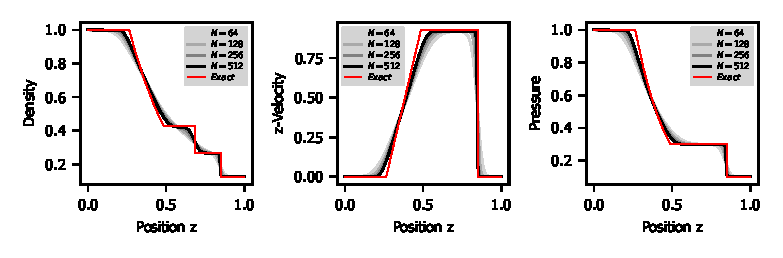
\includegraphics{sod_test.eps}
    \caption{Comparison of results for Sod shock tube case over different mesh refinements and analytical solution. $N$ stands for the number of cells along $z$-axis.}
    \label{fig:sod_test}
\end{figure}
\subsubsection{Uniform steady E-field}
The electric field comes into play in this testing where we expose electrons and ions to the uniform steady E-field $(0,0,1)$, namely unit vector along $z$-axis. For simplicity, two species are assumed to be equal in mass. The magnetic field is set to zero. Collisions among the species are neglected. Initially being static, the electrons and ions expect to be accelerated along the $z$-axis in opposite directions while keeping the temperature unchanged. Fig. \ref{fig:uniform_e_test} shows the behavior we expect. To be noticed is that the temperature slightly decreases over time due to numerical error, and the error is mitigated with mesh refinement.
\begin{figure}
    \centering
    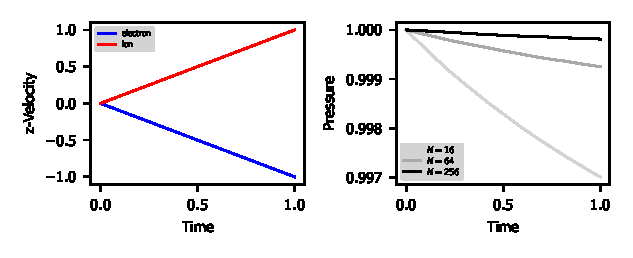
\includegraphics{uniform_E_test.eps}
    \caption{Result when a uniform background $\mathbf{E}$-field exists. The left figure shows the constant accelerations of electrons and ions. The right one indicates the slightly decreasing temperature due to numerical errors.}
    \label{fig:uniform_e_test}
\end{figure}

\subsubsection{Step voltage on anode}
In this case, we test the behavior of the Maxwell system when a step voltage is applied on the anode. Here we consider the domain to be dielectric and be devoid of plasma. In another word, we are dealing with the wave equation
\begin{equation} \label{equ:wave_eq} 
    \lambda^2\partial^2_t\mathbf{E} + \text{curl curl}\mathbf{E} = 0.
\end{equation}
The voltage on anode is given by
\begin{equation*}
    \varphi(t) = \frac{1}{2}\left(1+\text{tanh}\left( \frac{t - 1.0}{0.1}\right) \right).
\end{equation*}
We expect the electric field to produce oscillation with decaying magnitude. Besides, with Debye length $\lambda$ approaching zero, the damping becomes strong since the characteristic time scale is proportional to $\lambda$. Fig. \ref{fig:maxwell_test} (left) shows the $z$-component of $\mathbf{E}$-field at origin up to $t = 15$, and manifests such damping behavior.  
\begin{figure}
    \centering
    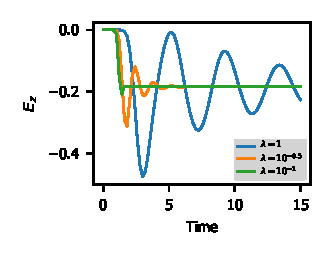
\includegraphics{maxwell_test.eps}
    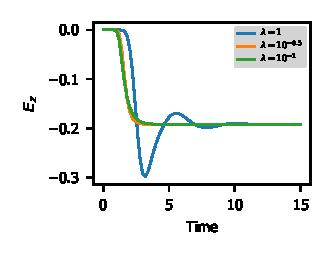
\includegraphics{maxwell_test2.eps}
    \caption{Axial component of the $\mathbf{E}$-field at origin point with step-like voltage on anode. The results are computed under the mesh with 16 cells along axial direction. (left) The domain is an ideal dielectric; (right) the domain is of constant conductivity.}
    \label{fig:maxwell_test}
\end{figure}

If we add to the conductivity of the material, and enforces the Ohm's law $\mathbf{J} = \sigma \mathbf{E}$, the problem to be solved becomes the wave equation with damping term
\begin{equation*}
    \lambda^2\partial^2_t\mathbf{E} + \sigma \partial_t \mathbf{E} - \nabla^2 \mathbf{E} = 0.
\end{equation*}
The introduction of conductivity causes dissipation and thus enhances the damping, as is shown in Fig. \ref{fig:maxwell_test} (right).

\section{Fully-coupled system}
We move on to test the performance of our fully-coupled Euler-Maxwell model (\ref{equ:maxwell_faraday_ap}) to (\ref{equ:current_ap}), and check its AP property. 

\subsection{Reduction to 1D}
On noticing the radial symmetry of the domain as well as boundary conditions, the governing equations defined at the axis of symmetry, namely $z$-axis in this case, can be tremendously simplified thanks to vanishing radial components of vector variables and radial derivatives. The Euler-Maxwell system at the axis of symmetry is formulated as 
\begin{align}
    &\partial_t n_* + \partial_z(n_*u_{*,z}) = 0, \\
    &\partial_t (n_* u_{*,z}) + \partial_z(n_*u_{*,z}^2) + \varepsilon_*^{-2} \partial_z P_* = \varepsilon_*^{-2}q_*n_*E_z, \\
    &\partial_t (n_*e_*) + \partial_z (n_* h_* u_{*,z}) = \varepsilon_*^{-2} q_* n_* u_{*,z} E_z, \\
    \lambda^2 &\partial_t E_z = \sum_* - q_* n_* u_{*,z}.
\end{align}
Recall that in section \ref{sec:two_fluid_model} the two-fluid model in 1D setting is discussed and verified. We take the results as reference solutions for the 1D reduction on the $z$-axis of the 3D model. With the same setting as is described in section \ref{sec:1d_two_fluid_numerical_results} and the vanishing anode potentials, we expect the results produced by the purely 1D model and 1D reduction of the 3D model to behave in a similar way, which is shown in Fig. \ref{fig:z_axis_reduction}.
\begin{figure}
    \centering
    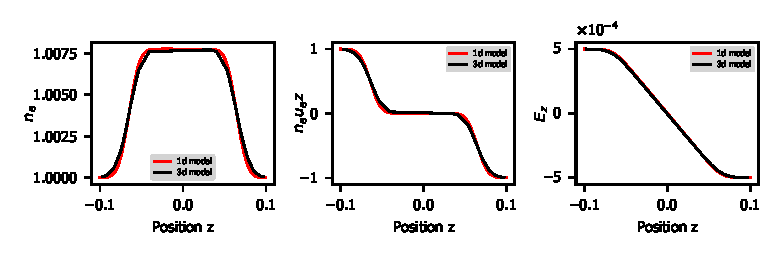
\includegraphics{z_axis_reduction.eps}
    \caption{Comparison of 1D two-fluid model and reduced 1D model on $z$-axis from 3D two-fluid model. The results are both generated on meshes with 64 cells along $z$-axis. No friction term exists. $t = 5 \times 10^{-4}.$}
    \label{fig:z_axis_reduction}
\end{figure}

\subsection{Numerical results in 3D} \label{chap:3d_problem}
Now comes the point to finally present the numerical results of the AP scheme on the Euler-Maxwell system in a 3D domain. To recap the problem setting and BCs, see Section \ref{sec:problem_description} and \ref{sec:numerical_experiement_bc}. We consider the two-fluid situation where the plasma is composed of electrons and ions. The mass ratio $m_i / m_e$ is equal to $10^4$. The friction term (\ref{equ:collision_rescaled}) is included with $\alpha^\text{coll} = 32$. Other effects like recombination or ionization are not considered yet.  

The initial state is
\begin{equation*}
    n_i(x,y,z,0) = n_e(x,y,z,0) = 1, \ \ \  p_i(x,y,z,0) = p_e(x,y,z,0) = 1.
\end{equation*}
All the other quantities are vanishing initially. The cathode is grounded, and the anode has potential 1.0 throughout the simulation, namely $\varphi^-(t) = 0, \varphi^+(t) = 1.0$. It is intended to see how a stationary system responds to an applied voltage. We would like to remark that such an initial state is conforming to the BCs as well as the quasi-neutral condition $\rho = 0$ so that the quasi-neutrality $\lambda  = 0$ would not incur any initial layer. 

In Fig. \ref{fig:3d_vec_field_E_B_ue} we present the vector fields of the numerical solutions for $\lambda = 1.0, 0.01, 0$ at $t = 0.1$, aiming to give an intuitive visualization. First of all, one \emph{a priori} expects the rotational symmetry in the solutions, which serves as a basic criterion to justify the results. In terms of the 3D structure of the electromagnetic fields, the electric field points from the anode to the cathode, and the magnetic field is spiral-shaped and orthogonal to the electric field. The electrons move in the inverse direction of the electric field. Regarding the asymptotic behavior of the AP scheme, the primary concern is its validity in the limiting case. For this case, the scheme manages to produce a meaningful numerical solution when $\lambda = 0$. Besides, by comparing the solutions for different $\lambda$, the smooth transition from the non-neutrality to quasi-neutrality is observed, which is an implication that the scheme reproduces the asymptotic behavior of the analytical solutions from the non-neutral model to the quasi-neutral one.
\begin{figure}
    \centering
    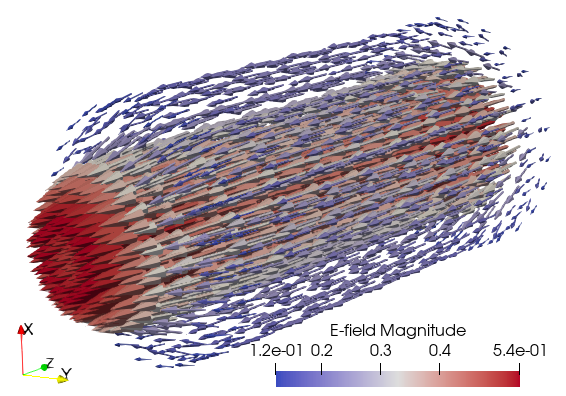
\includegraphics[scale=0.35]{E_lambda_1.png}
    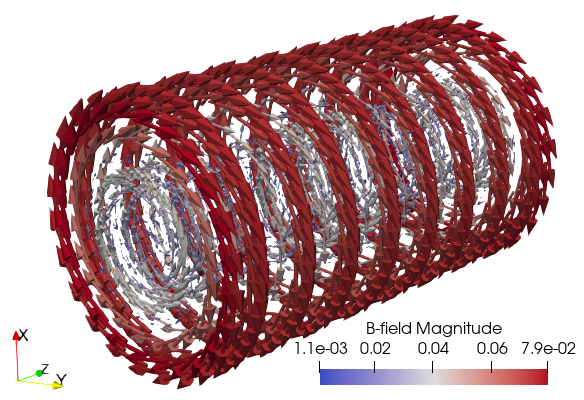
\includegraphics[scale=0.35]{B_lambda_1.png}
    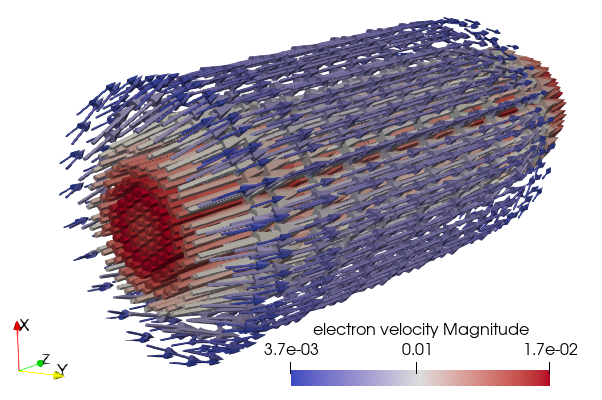
\includegraphics[scale=0.35]{ue_lambda_1.png} \\
    (a) $\lambda = 1.0$ \\
    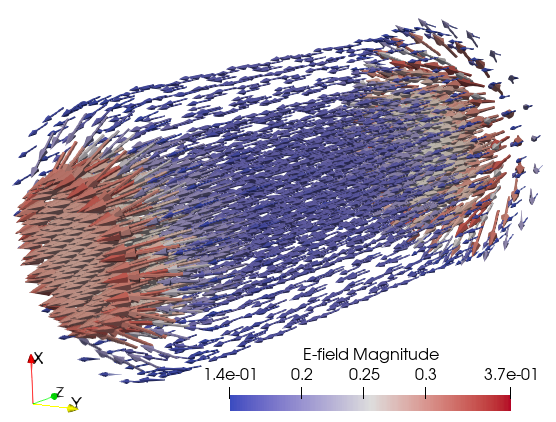
\includegraphics[scale=0.35]{E_lambda_1e-2.png}
    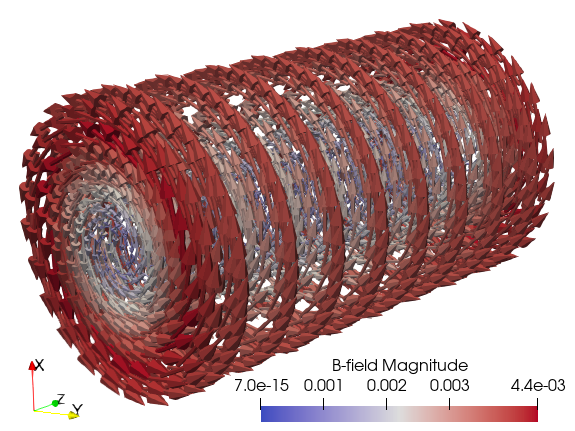
\includegraphics[scale=0.35]{B_lambda_1e-2.png}
    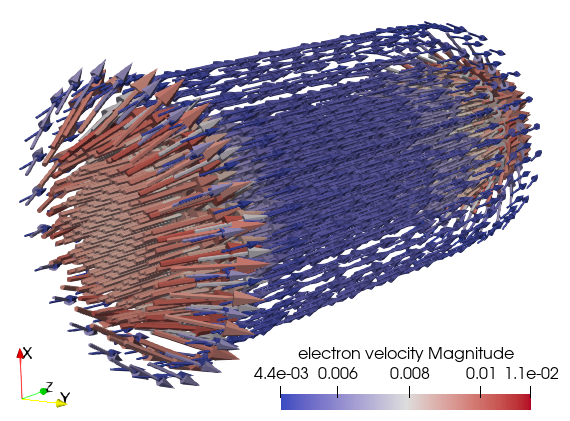
\includegraphics[scale=0.35]{ue_lambda_1e-2.png} \\
    (b) $\lambda = 0.01$ \\
    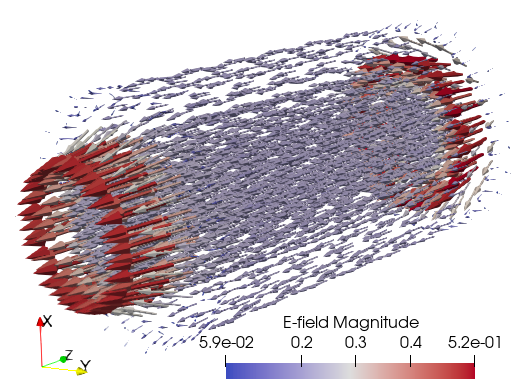
\includegraphics[scale=0.35]{E_lambda_0.png}
    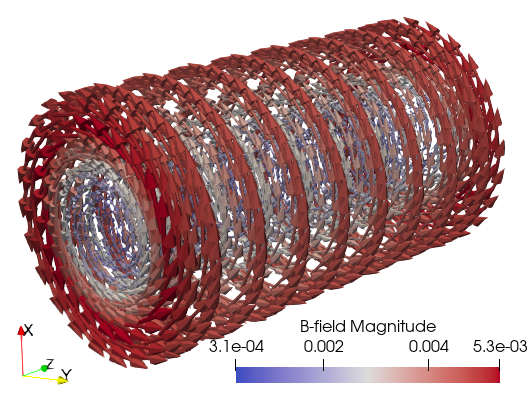
\includegraphics[scale=0.35]{B_lambda_0.png}
    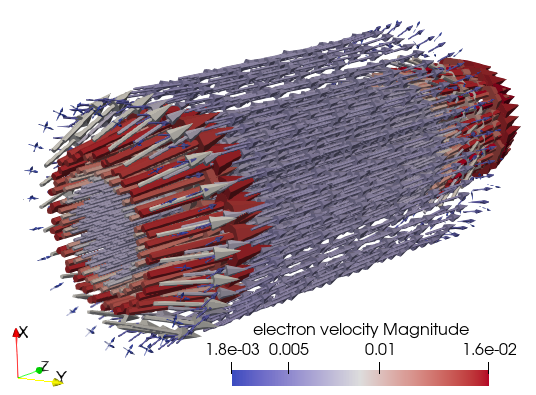
\includegraphics[scale=0.35]{ue_lambda_0.png} \\
    (c) $\lambda = 0$
    \caption{Snapshots of the $\mathbf{E}$-field, $\mathbf{B}$-field, and $\mathbf{u}_e$ for different $\lambda$ at $t = 10$ based on a primal mesh with 1920 cells (8 cells along $z$-axis). } 
    \label{fig:3d_vec_field_E_B_ue}
\end{figure}

We perform the grid study and show the result in Fig. \ref{fig:grid_study_3d}. Meshes with different refinement levels are tested for $\lambda = 1$ and $0.1$ at $t = 1$, and the norms of the quantities are calculated. Due to the high computational cost incurred by the curse of dimensionality, only meshes with limited size are tested and the asymptotic regime of the grid study might be not reached. Nevertheless, it still helps to reveal the independence of solutions with respect to meshes --- the norms of electron density and the magnetic field do not deviate in a divergent manner. The exception of the norm of the electric field possibly results from the singularity caused by the interface of the contacting and insulating surfaces, as will be seen later. 
In Fig. \ref{fig:grid_study_3d_clip_lambda-1e-1} and \ref{fig:grid_study_3d_clip_lambda-0}, we plot the distribution of certain quantities at the cross-section based on different meshes for $\lambda = 0.1$ and $0$ at $t = 1$. Thanks to the rotational symmetry of the problem, the solution at the cross-section suffices to characterize the whole solution. The figures again demonstrate the stability of the numerical solutions with respect to mesh refinement in the sense that qualitatively the same solutions are produced by a series of meshes of different sizes. We would like to point out that singularity arises in the $\mathbf{E}$-field at the interface of contacting and insulating surfaces (two points at the left end and two at the right end). In numerical experiments, we observe an increasing magnitude of the $\mathbf{E}$-field at these points as the mesh is refined. Furthermore, it is noted from Fig. \ref{fig:grid_study_3d_clip_lambda-0} (last two rows) that when $\lambda = 0$, the charges carried by ions and electrons cancel out everywhere as indicated by the quasi-neutral condition $\rho = 0$.

\begin{figure}
    \centering
    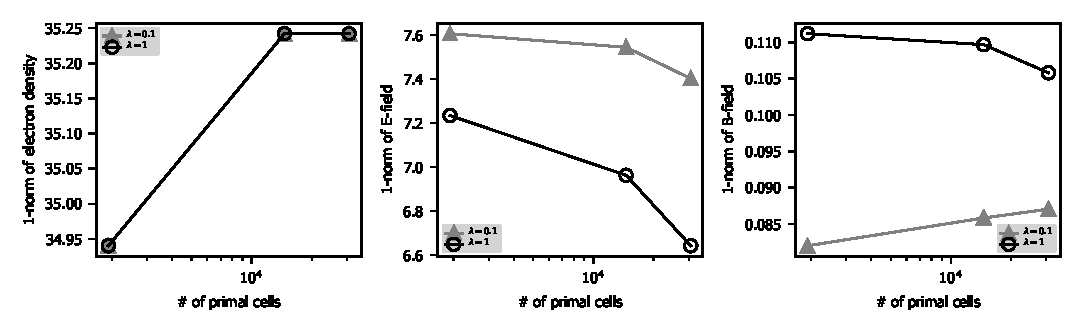
\includegraphics[scale=0.9]{norm_vs_nCell-T_1.eps}
    \caption{1-norms of quantities with respect to different mesh size: The results are computed for $\lambda = 1$ and $0.1$ at $t = 1$.}.
    \label{fig:grid_study_3d}
\end{figure}

\begin{figure}
    \centering
    Refinement 1\hspace{2.5cm}Refinement 2\hspace{2.5cm}Refinement 3\hspace{1cm}
    
    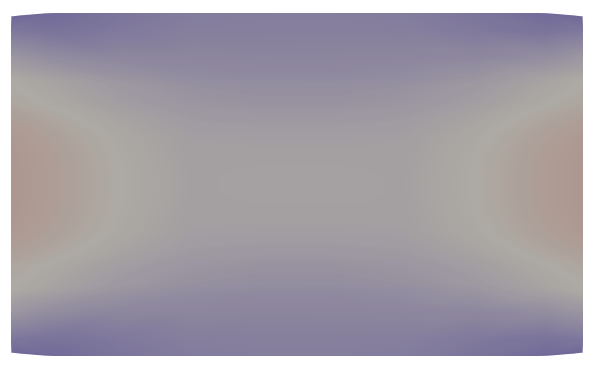
\includegraphics[scale=0.27]{clip_E_T-1_lambda-1e-1_8-2-2.png}
    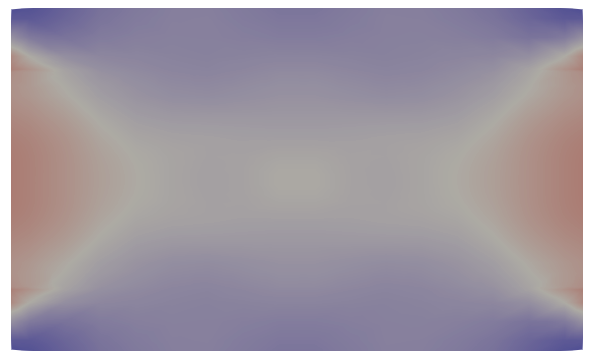
\includegraphics[scale=0.27]{clip_E_T-1_lambda-1e-1_16-3-3.png}
    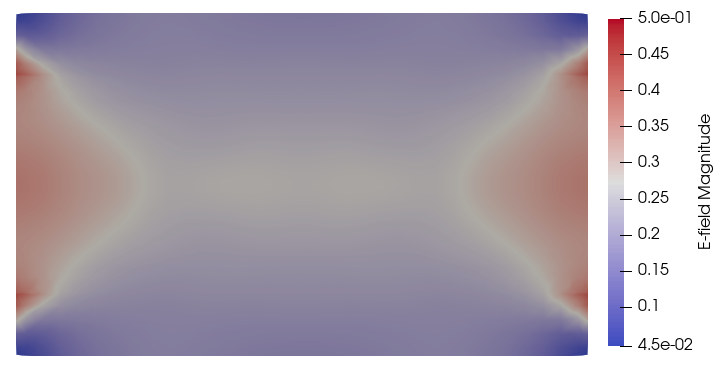
\includegraphics[scale=0.27]{clip_E_T-1_lambda-1e-1_32-3-4.png}
    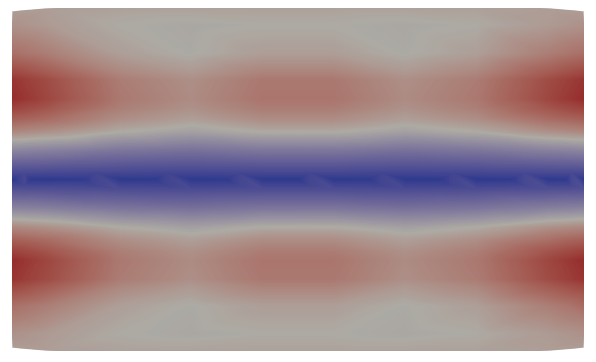
\includegraphics[scale=0.27]{clip_B_T-1_lambda-1e-1_8-2-2.png}
    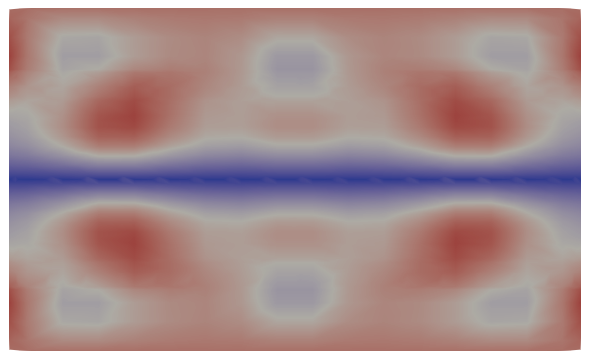
\includegraphics[scale=0.27]{clip_B_T-1_lambda-1e-1_16-3-3.png}
    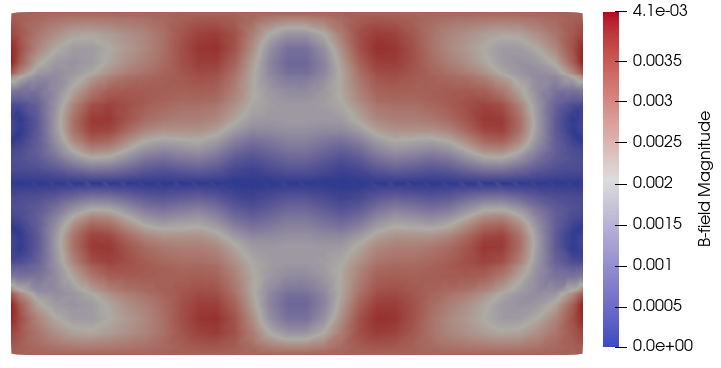
\includegraphics[scale=0.27]{clip_B_T-1_lambda-1e-1_32-3-4.png}
    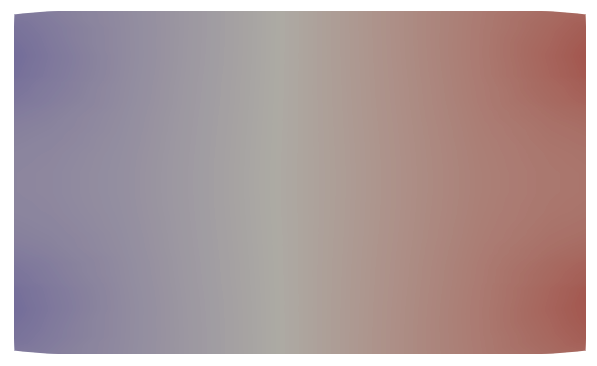
\includegraphics[scale=0.27]{clip_ne_T-1_lambda-1e-1_8-2-2.png}
    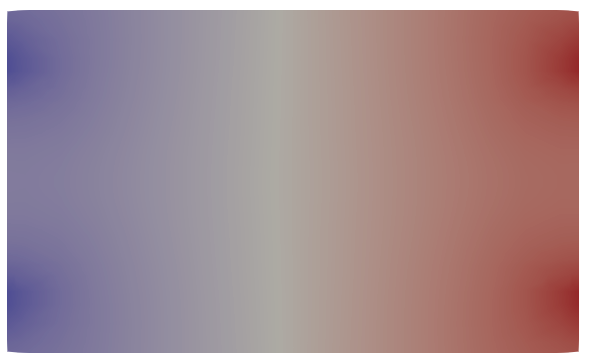
\includegraphics[scale=0.27]{clip_ne_T-1_lambda-1e-1_16-3-3.png}
    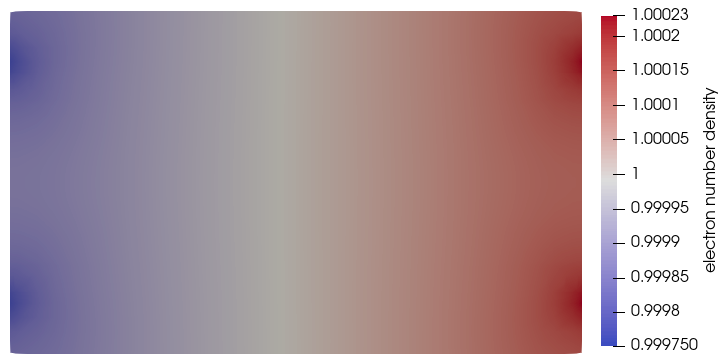
\includegraphics[scale=0.27]{clip_ne_T-1_lambda-1e-1_32-3-4.png}
    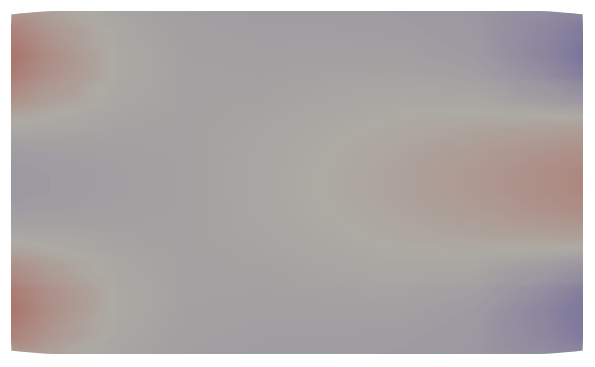
\includegraphics[scale=0.27]{clip_ni_T-1_lambda-1e-1_8-2-2.png}
    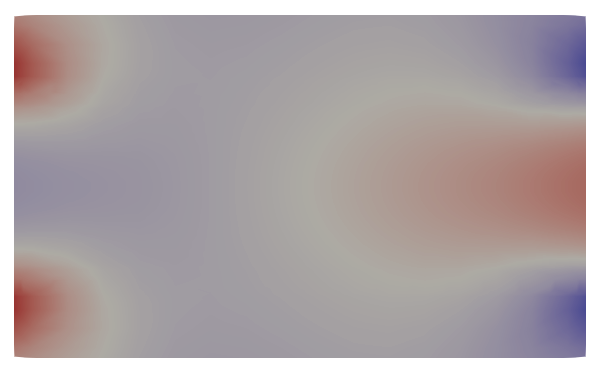
\includegraphics[scale=0.27]{clip_ni_T-1_lambda-1e-1_16-3-3.png}
    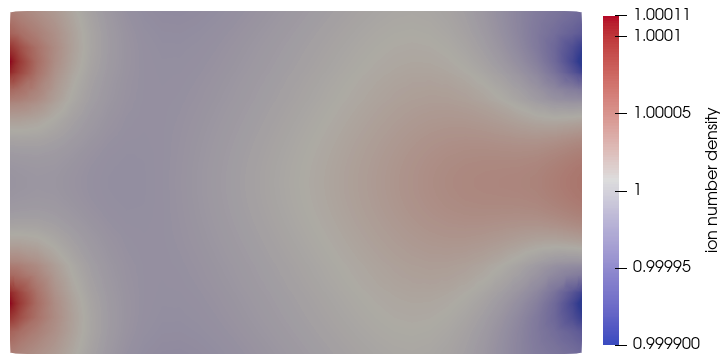
\includegraphics[scale=0.27]{clip_ni_T-1_lambda-1e-1_32-3-4.png}
    \caption{Quantities at the cross-section generated by meshes with different refinement level. Refinement 1: 1920 primal cells; Refinement 2: 14592 primal cells; Refinement 3: 30720 primal cells. The snapshots are computed for $\lambda = 0.1$ at $t = 1$.}
    \label{fig:grid_study_3d_clip_lambda-1e-1}
\end{figure}

\begin{figure}
    \centering
    Refinement 1\hspace{2.5cm}Refinement 2\hspace{2.5cm}Refinement 3\hspace{1cm}
    
    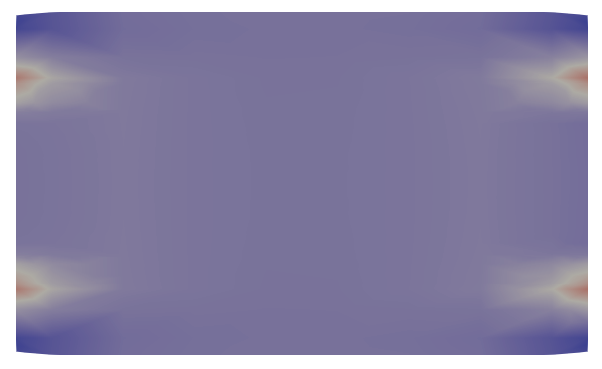
\includegraphics[scale=0.27]{slice_E_T-1_lambda-0_8-2-2.png}
    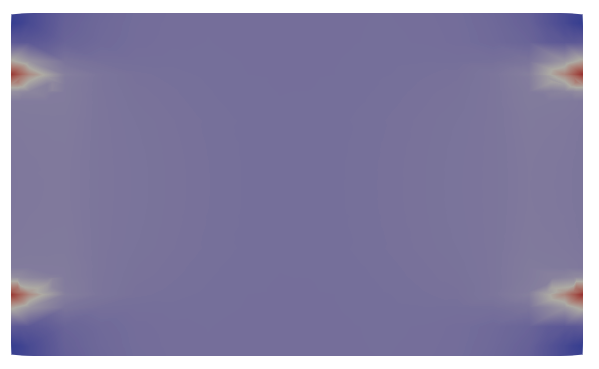
\includegraphics[scale=0.27]{slice_E_T-1_lambda-0_16-3-3.png}
    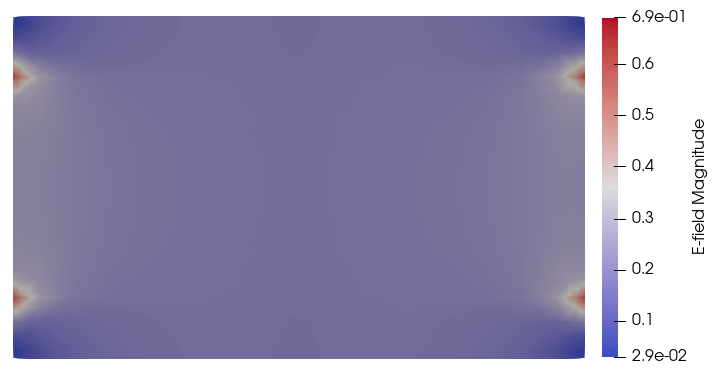
\includegraphics[scale=0.27]{slice_E_T-1_lambda-0_32-3-4.png}
    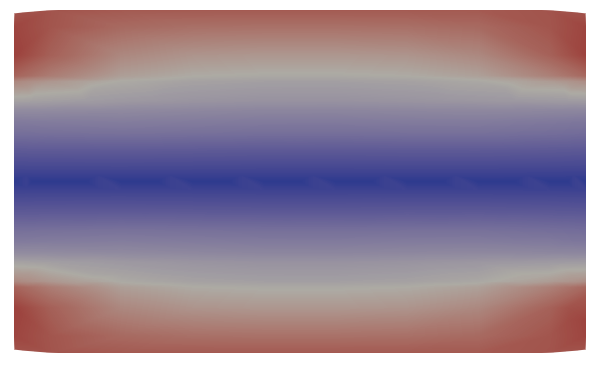
\includegraphics[scale=0.27]{slice_B_T-1_lambda-0_8-2-2.png}
    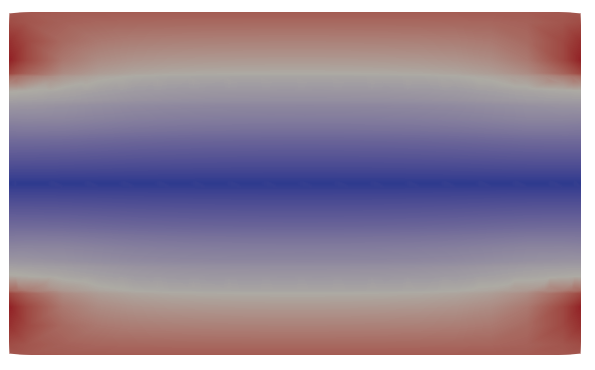
\includegraphics[scale=0.27]{slice_B_T-1_lambda-0_16-3-3.png}
    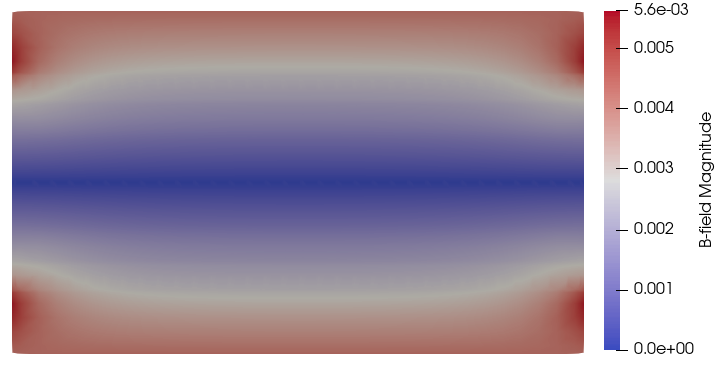
\includegraphics[scale=0.27]{slice_B_T-1_lambda-0_32-3-4.png}
    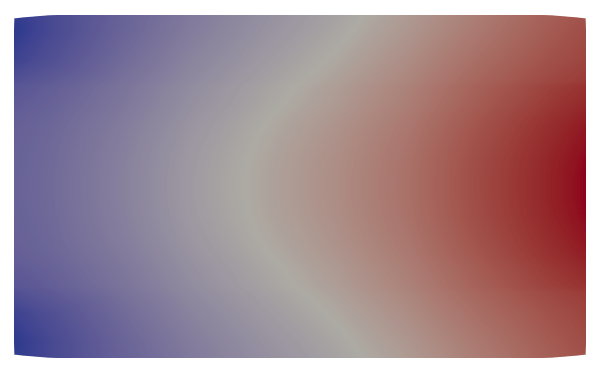
\includegraphics[scale=0.27]{slice_ne_T-1_lambda-0_8-2-2.png}
    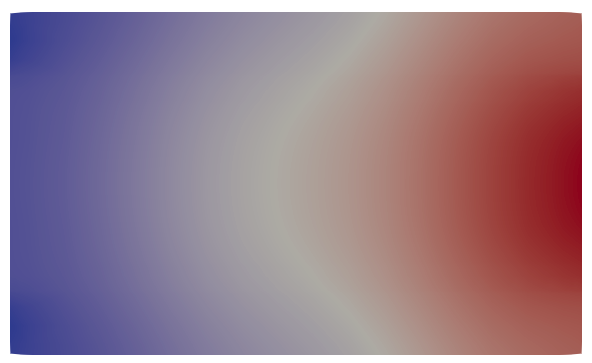
\includegraphics[scale=0.27]{slice_ne_T-1_lambda-0_16-3-3.png}
    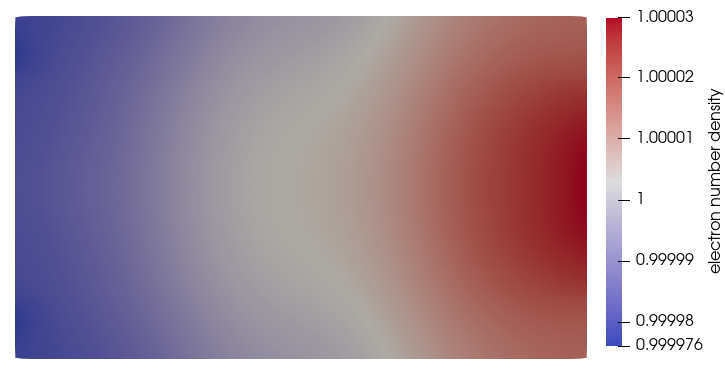
\includegraphics[scale=0.27]{slice_ne_T-1_lambda-0_32-3-4.png}
    \includegraphics[scale=0.27]{slice_ni_T-1_lambda-0_8-2-2.png}
    \includegraphics[scale=0.27]{slice_ni_T-1_lambda-0_16-3-3.png}
    \includegraphics[scale=0.27]{slice_ni_T-1_lambda-0_32-3-4.png}
    \caption{Quantities at the cross-section generated by meshes with different refinement level. Refinement 1: 1920 primal cells; Refinement 2: 14592 primal cells; Refinement 3: 30720 primal cells. The snapshots are computed for $\lambda = 0$ at $t = 1$.}
    \label{fig:grid_study_3d_clip_lambda-0}
\end{figure}

To inspect how the system evolves, we extract the time histories of certain quantities at the origin (the center of the tube) up to $t = 10$ and display them in Fig. \ref{fig:origin-data_vs_time}. Being originally at rest, the system is excited by the suddenly applied voltage and generates oscillations that dampen over time. In general, a large value of $\lambda$ leads to stronger oscillations with larger amplitude whereas smaller $\lambda$ incurs more damping and the system rapidly reaches a steady state. It is a reflection of the shielding effect of plasma which is characterized by the Debye length. It can also be noticed that the electron velocity becomes steady much sooner than ion velocity, which is a consequence of the huge difference in inertia. Besides, the convergence of the discrete model as $\lambda \rightarrow 0$ can be observed---the solution becomes steady over time.
\begin{figure}
    \centering
    \includegraphics[scale=0.9]{origin-data_vs_time.eps}
    \caption{Time histories of quantities at the origin for different $\lambda$. The simulation is done on a mesh with 1920 primal cells with 8 layers along $z$-axis.}
    \label{fig:origin-data_vs_time}
\end{figure}

A critical sign of quasi-neutrality is the vanishing charge. In fact, in Section \ref{sec:quasi-neutral_limit} we discuss the limiting model where $\rho = 0$ is satisfied. To examine that, the quantities at the $z$-axis over different $\lambda$ are provided in Fig. \ref{fig:zaxis-data_vs_z-T_10}. The right figure demonstrates the approaching and eventual coincidence of electron and ion densities as $\lambda \rightarrow 0$. Furthermore, with relatively small but non-zero $\lambda$, the bulk of the plasma is approximately neutral while the area near the electrodes is not, which is known as a plasma sheath and within such an area the quasi-neutrality is usually inappropriate.
\begin{figure}
    \centering
    \includegraphics{zaxis-data_vs_z-T_10.eps}
    \caption{Quantities along $z$-axis for different $\lambda$: The results are computed at $t = 10$ on a mesh with 1920 primal cells with 8 layers along $z$-axis.}.
    \label{fig:zaxis-data_vs_z-T_10}
\end{figure}

In Fig. \ref{fig:clip-ne-nue-T_10} the distribution of the electron number density and velocity at the cross-section is displayed. In the non-neutral case, the electrons accumulate near the anode, and the velocity is distributed rather uniformly. With the model approaching quasi-neutrality $\lambda = 0$, the electrons move slower in the bulk area while they are accelerated to high speed at the edge of electrodes, and they tend to accumulate in the middle pass.
\begin{figure}
    \centering
    \begin{subfigure}[b]{0.4\textwidth}
        \centering
        \includegraphics[scale=0.4]{clip-ne-nue-T_10-lambda_1.png}
        \caption{$\lambda = 1$}
    \end{subfigure}
    \begin{subfigure}[b]{0.4\textwidth}
        \centering
        \includegraphics[scale=0.4]{clip-ne-nue-T_10-lambda_1e-1.png}
        \caption{$\lambda = 0.1$}
    \end{subfigure}
    \begin{subfigure}[b]{0.4\textwidth}
        \centering
        \includegraphics[scale=0.4]{clip-ne-nue-T_10-lambda_1e-2.png}
        \caption{$\lambda = 0.01$}
    \end{subfigure}
    \hspace{0.2cm}
    \begin{subfigure}[b]{0.4\textwidth}
        \centering
        \includegraphics[scale=0.38]{clip-ne-nue-T_10-lambda_0.png}
        \caption{$\lambda = 0$}
    \end{subfigure}
    \caption{Electron number density and velocity vector at the cross-section. The results are computed at $t = 10$ on a mesh with 1920 primal cells with 8 layers along $z$-axis. The velocity vector lengths, which indicates the magnitude, are rescaled by the same factor.}
    \label{fig:clip-ne-nue-T_10}
\end{figure}

\section{Summary}
To evaluate the performance of the scheme (\ref{equ:maxwell_faraday_ap}) to (\ref{equ:euler_ap}), we need to examine the two criterion in Definition \ref{def:ap} which states the asymptotic stability and consistency. Both properties are \emph{experimentally} checked in a 3D setting. The former one, referring to the unconditional stability on $\lambda$, is confirmed as the program achieves meaningful solutions for arbitrary $\lambda$ without adjusting the time step size. The latter one requires the convergence of the limit scheme to the limit model, which is supported by two facts: the smooth transition of numerical solutions over $\lambda \in [0,1]$ and the conformity of the quasi-neutral condition $n_i = n_e$. 

\chapter{Extension to Insulating Domain}
As is mentioned in Section \ref{sec:impact_insulating_domain}, the scheme so far could not directly handle the case with an insulating domain $\Omega_I$ where no plasma fluid is there. An example is shown in Fig. \ref{fig:sketch_domain_fusch}. Now the plasma domain is enclosed by a insulating sleeve. 

We repeat the dilemma again: the scheme fails for $\lambda \rightarrow 0$. The Maxwell system in $\Omega_I$ is    
\begin{align}
    \partial_t \mathbf{B} + \nabla \times \mathbf{E} &= 0, \label{equ:ex_1}\\ 
    \lambda^2 \partial_t \mathbf{D} - \nabla \times \mathbf{H} &= 0,  \label{equ:ex_2}\\
    \nabla \cdot \mathbf{B} &= 0, \label{equ:ex_3}\\
    \lambda^2 \nabla \cdot \mathbf{D} &= 0 \label{equ:ex_4}.
\end{align}
In non-neutral regime, namely $\lambda = \mathcal{O}(1)$, the Maxwell system in $\Omega_I$ is well-posed and Gauss's laws (\ref{equ:ex_3}) (\ref{equ:ex_4}) are redundant. Therefore, they are \emph{implicitly} satisfied (up to numerical errors) in the scheme. Nonetheless, the quasi-neutral limit $\lambda \rightarrow 0$ dismisses the implicit fulfillment of Gauss's law for electric field (\ref{equ:ex_4}) through Amper\`{e}'s law (\ref{equ:ex_2}). A crucial observation is that formally letting $\lambda \rightarrow 0$ makes (\ref{equ:ex_4}) degenerate, but the divergence-free condition of $\mathbf{D}$-field is always satisfied since the system is divergent as $\lambda \rightarrow 0$ [cite something]. 

The remedy is to \emph{explicitly} include the divergence-free constraint in the scheme for any value of $\lambda$:  
\begin{align}
    \partial_t \mathbf{B} + \nabla \times \mathbf{E} &= 0, \label{equ:ex_5}\\ 
    \lambda^2 \partial_t \mathbf{D} - \nabla \times \mathbf{H} &= 0,  \label{equ:ex_6}\\
    \nabla \cdot \mathbf{D} &= 0 \label{equ:ex_7}.
\end{align}

With the divergence-free constraint (\ref{equ:ex_7}), we have more equations than unknowns, which can be resolved by introducing a Lagrange multiplier $p$ as follows:
\begin{align}
    \partial_t \mathbf{B} + \nabla \times \mathbf{E} &= 0, \label{equ:ex_8}\\ 
    \lambda^2 \partial_t \mathbf{D} - \nabla \times \mathbf{H} + \colorbox{orange!20}{$\nabla p$} &= 0,  \label{equ:ex_9}\\
    \nabla \cdot \mathbf{D} &= 0 \label{equ:ex_10},
\end{align}
supplemented with the boundary condition $p = 0$ on $\partial\Omega_I$. One can check that (\ref{equ:ex_8})-(\ref{equ:ex_10}) are equivalent to (\ref{equ:ex_5})-(\ref{equ:ex_7}) by verifying that $p = 0$ in $\Omega_I$. This is done by taking the divergence of (\ref{equ:ex_9}) such that the Laplace equation of $p$ with zero Dirichlet boundary condition gives vanishing $p$. 

The discretization of the Maxwell system in the insulating domain then becomes
\begin{align*}
    \delta_m^{-1} (\mathbf{b}^{m+1} - \mathbf{b}^m) + \mathbb{C}\mathbf{e}^{m+1} &= 0, \\
    \lambda^2\delta_m^{-1} (\Tilde{\mathbf{d}}^{m+1} - \Tilde{\mathbf{d}}^m) - \Tilde{\mathbb{C}}\Tilde{\mathbf{h}}^{m+1} + \colorbox{orange!20}{$\mathbb{H} \mathbb{G} \mathbf{p}^{m+1}$} &= 0 \\
    \Tilde{\mathbb{D}} \Tilde{\mathbf{d}}^{m+1} &= 0.
\end{align*}
where $\mathbb{H}$ is the discrete Hodge operator (matrix\footnote{In our case where the orthogonal mesh pair is used, it is diagonal.}) responsible for transforming any primal-edge-integrated variables to dual-face-integrated ones; the vector $\mathbf{p}$ is the discrete representation of $p$ and is defined on primal vertices lying in $\Omega_I$.

\begin{figure}
    \centering
    \begin{minipage}{0.5\textwidth}
\resizebox{\textwidth}{!}{
    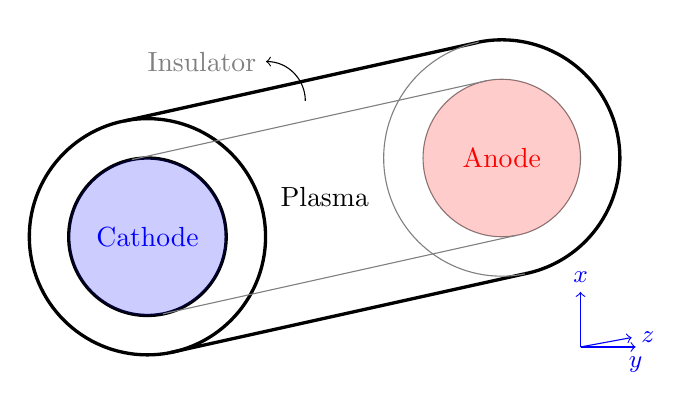
\begin{tikzpicture}
    \coordinate (O1) at (0,0);
    \draw[very thick] (O1) circle (1) node[blue] {Cathode};
    \fill[blue, opacity=0.2] (O1) circle (1);
    \draw[very thick] (O1) circle (1.5);
    \coordinate (O2) at (4.5,1) ;
    \draw[gray] (O2) circle (1);
    \node at (O2) {\textcolor{red}{Anode}};
    \node at (barycentric cs:O1=1,O2=1) {Plasma}; 
    \fill[red, opacity=0.2] (O2) circle (1);
    \coordinate (S1) at ([shift={(-0.196,0.98)}]O1);
    \coordinate (S2) at ([shift={(-0.196,0.98)}]O2);
    \coordinate (P1) at ([shift={(0.196,-0.98)}]O1);
    \coordinate (P2) at ([shift={(0.196,-0.98)}]O2);
    \draw[gray] (S1) -- (S2);
    \draw[gray] (P1) -- (P2);
    \coordinate (SS1) at ([shift={({-0.196*1.5},{0.98*1.5})}]O1);
    \coordinate (SS2) at ([shift={({-0.196*1.5},{0.98*1.5})}]O2);
    \coordinate (PP1) at ([shift={({0.196*1.5},{-0.98*1.5})}]O1);
    \coordinate (PP2) at ([shift={({0.196*1.5},{-0.98*1.5})}]O2);
    \draw[very thick] (SS1) -- (SS2);
    \draw[very thick] (PP1) -- (PP2); 
    \draw[gray] (SS2) arc (101.31:180+101.31:1.5);
    \draw[very thick] (PP2) arc (101.31-180:101.31:1.5);
    \draw[-to] (barycentric cs:SS1=1,SS2=1,S1=1,S2=1) to[out=90,in=0] ([shift={(-0.5,0.5)}]barycentric cs:SS1=1,SS2=1,S1=1,S2=1) node[left, gray] {Insulator};
    \begin{scope}[shift={(5.5,-1.4)}]
    \draw[blue, -to] (0,0) -- (0.65,0.12) node[right]{\small $z$};
    \draw[blue, -to] (0,0) -- (0,0.7) node[above]{\small $x$};
    \draw[blue, -to] (0,0) -- (0.7,0) node[below]{\small $y$};
    \end{scope}
    \end{tikzpicture}}
\end{minipage}
\begin{minipage}{0.49\textwidth}
    \resizebox{1.1\textwidth}{!}{ 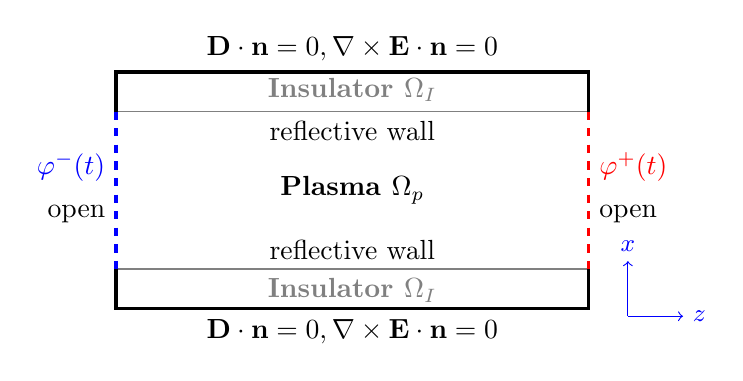
\begin{tikzpicture}
        \coordinate (A1) at (0,1.5);
        \coordinate (A2) at (0,1);
        \coordinate (A3) at (0,-1);
        \coordinate (A4) at (0,-1.5);
        \coordinate (B1) at (6,1.5);
        \coordinate (B2) at (6,1);
        \coordinate (B3) at (6,-1);
        \coordinate (B4) at (6,-1.5);
        \draw[gray] (A2) -- node[above]{\textbf{Insulator $\Omega_I$}} node[black, below]{reflective wall} (B2);
        \draw[gray] (A3) -- node[below]{\textbf{Insulator $\Omega_I$}} node[black, above]{reflective wall} (B3);
        \draw[very thick] (A2) -- (A1) -- node[above]{$\mathbf{D} \cdot \mathbf{n} = 0, \nabla \times \mathbf{E} \cdot \mathbf{n} = 0$}  (B1) -- (B2);
        \draw[very thick] (A3) -- (A4) -- node[below]{$\mathbf{D} \cdot \mathbf{n} = 0, \nabla \times \mathbf{E} \cdot \mathbf{n} = 0$} (B4) -- (B3);
        \draw[very thick, dashed, blue] (A2) -- node[left, yshift=0.3cm] {$\varphi^-(t)$} node[left, yshift=-0.3cm] {\textcolor{black}{open}} (A3);
        \draw[very thick, dashed, red]  (B2) -- node[right, yshift=0.3cm]  {$\varphi^+(t)$} node[right, yshift=-0.3cm] {\textcolor{black}{open}}  (B3);
        \node at (3,0) {\textbf{Plasma $\Omega_p$}};
        \begin{scope}[shift={(6.5,-1.6)}]
        \draw[blue, -to] (0,0) -- (0,0.7) node[above]{\small $x$};
        \draw[blue, -to] (0,0) -- (0.7,0) node[right]{\small $z$};
        \end{scope}
    \end{tikzpicture}}
\end{minipage}
    \caption{Caption}
    \label{fig:ex}
\end{figure}

The setting of the numerical test is sketched in Fig. \ref{fig:ex}. The initial conditions keep unchanged as Section \ref{chap:3d_problem}.  

As predicted in the analytic case, the Lagrange multiplier $p$ is approximately zero (in the order of $\mathcal{O}(10^{-12})$) in the numerical test. The introduction of the surrounding insulator sleeve does not qualitatively alters the 3D structure of the resulting electromagnetic fields (see Fig. \ref{fig:3d_vec_field_E_B_ue}), which are therefore omitted here. In Fig. \ref{fig:time_history_extend} we demonstrate how quantities at the center of the cylinder evolve with time. Comparison with its counterpart Fig. \ref{fig:origin-data_vs_time} shows many similarities. An interesting point is that now the ions move towards the anode, which is not nonphysical since the frictional force could be stronger than the electric force. What matters is the capability of the scheme to handle the quasi-neutral limit.
\begin{figure}
    \centering
    \includegraphics[scale=0.9]{origin_data-vs-time_withInsulator.eps}
    \caption{Time histories of quantities at the origin for different value of $\lambda$. The simulations are done on a mesh with 3840 primal cells with 16 layers along $z$-axis. Compared to fig. \ref{fig:origin-data_vs_time}, an insulating domain is included in this case.}
    \label{fig:time_history_extend}
\end{figure}




\chapter{Conclusion}
We generalize the AP scheme proposed in \cite{degond_2012}, which is originally designed to handle the quasi-neutrality of the Euler-Maxwell system and applied to problems in 1D, to a 3D scenario. Such generalization has been partially done in \cite{fuchs_2021}, and yet an inconsistency in the limiting case remains unsolved. Based upon the framework built by \cite{fuchs_2021}, this thesis proposes several modifications to the algorithm and the targeting problems.    

The generalized scheme incorporates FIT and FVM for spatial discretization of Maxwell's equations and the Euler equations. The time discretization is of critical significance in attaining AP property, and the choice of implicit terms conforms to the mentioned references. Additionally, the collision between species is included. Substantial efforts are put on issues related to the boundary. We enforce the BCs under the framework of FIT by introducing auxiliary mesh facets and quantities at the boundary. Furthermore, we identify the proper BCs that are essential for the well-posedness of the Euler-Maxwell system over different regimes. The detailed strategy to assemble the linear system due to the implicitness is presented. The 3D scheme is first validated on the subsystems and is compared to its corresponding 1D discrete model. Solutions performed on the fully-coupled system for $\lambda$ ranging in $[0,1]$ show a smooth transition from the non-neutral model to the quasi-neutral one, which demonstrates that our scheme is AP.

Apart from the implementation of the scheme in 3D, the definition and property of AP schemes are rephrased in a more definite way. Despite a large amount of literature discussing AP schemes, the definition differs from paper to paper and remains vague. In this thesis, we summarize AP properties by two features: asymptotic-stability and asymptotic-consistency, which refer to the unconditional stability on the asymptotic parameter, and convergence of the scheme in the limiting case. We formulate two propositions as an attempt to unveil the connection between these two aspects---the second one might be relaxed by only requiring consistency under certain assumptions. 

Future works could be carried out in the following directions. As is discussed in Section \ref{sec:impact_insulating_domain}, the failure arising from the insulating solid domain could be remedied by enforcing $\nabla \cdot \mathbf{D}$ = 0, which is worth pursuing. In terms of implementation, the algorithm is not yet optimized. As the bottleneck, solving the large sparse linear systems consumes nearly all the computation time. The matrix assembly might be smarter such that the resulting linear system possesses certain desired properties, e.g. symmetric positive-definite, and hence a faster solver can be invoked. Besides, the present AP scheme is of first-order in accuracy. The combination of high-order schemes and the AP property is a potential challenge since several issues, e.g. the intra-mesh interpolation of the electromagnetic fields and the discrete material law, could undermine the accuracy. One can also contemplate incorporating the AP property into other numerical frameworks like FEM. Regarding the design of AP schemes, the approaches so far are mostly heuristic and specific to the given problem. A unified strategy of construction and verification is still to be explored.

\begin{appendices}
\chapter{Rusanov Flux in 3D} \label{app:flux}
Consider the Euler equations
\begin{align} \label{equ:euler}
    \partial_t
    \begin{bmatrix}
    \rho \\
    \rho \mathbf{u} \\
    E
    \end{bmatrix}
    + \nabla \cdot
    \begin{bmatrix}
    \rho \mathbf{u} \\
    \rho \mathbf{u} \otimes \mathbf{u} + p\mathbb{I} \\
    (E+p)\mathbf{u}
    \end{bmatrix}
    = 0.
\end{align}
In 3D Cartesian coordinate system, it reads 
\begin{align} \label{equ:euler_xyz}
    \partial_t \mathbf{U} + \partial_x \mathbf{F}^x(\mathbf{U}) + \partial_y \mathbf{F}^y(\mathbf{U}) + \partial_z \mathbf{F}^z(\mathbf{U}) = 0.
\end{align}
where
\begin{equation*}
    \mathbf{U} =
    \begin{bmatrix}
    \rho \\
    \rho u_x \\
    \rho u_y \\
    \rho u_z \\
    E
    \end{bmatrix}, \ \ \ 
    \mathbf{F}^x(\mathbf{U}) =
    \begin{bmatrix}
    \rho u_x \\
    \rho u_x^2 + p \\
    \rho u_y u_x  \\
    \rho u_z u_x \\
    (E + p)u_x
    \end{bmatrix}, \ \ \ 
    \mathbf{F}^y(\mathbf{U}) =
    \begin{bmatrix}
    \rho u_y \\
    \rho u_x u_y \\
    \rho u_y^2 + p \\
    \rho u_z u_y \\
    (E + p)u_y
    \end{bmatrix}, \ \ \ 
    \mathbf{F}^z(\mathbf{U}) =
    \begin{bmatrix}
    \rho u_z \\
    \rho u_x u_z  \\
    \rho u_y u_z  \\
    \rho u_z^2  + p\\
    (E + p)u_z
    \end{bmatrix}
\end{equation*}
\begin{figure}
    \centering
    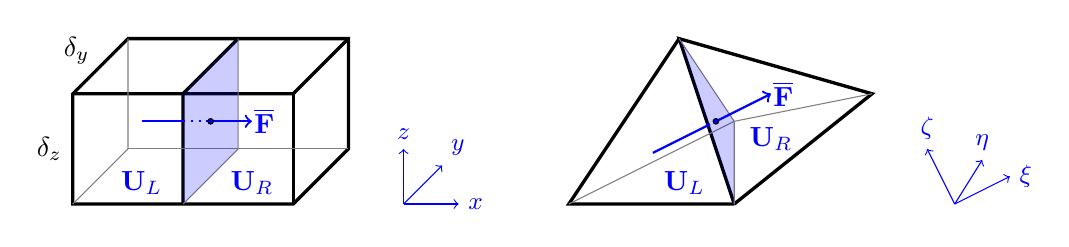
\begin{tikzpicture}[scale=0.7]
        \coordinate (A1) at (0,0);
        \coordinate (A2) at (2,0);
        \coordinate (A3) at (3,1);
        \coordinate (A4) at (3,3);
        \coordinate (A5) at (1,3);
        \coordinate (A6) at (-1,3);
        \coordinate (A7) at (-2,2);
        \coordinate (A8) at (-2,0);
        \coordinate (A10) at (0,2);
        \coordinate (A11) at (2,2);
        \coordinate (A12) at (-1,1);
        \coordinate (A13) at (1,1);
        \draw[very thick] (A1) -- (A2) -- (A3) -- (A4) -- (A5) -- (A6) -- node[left, yshift=2mm]{$\delta_y$} (A7) -- node[left]{$\delta_z$} (A8) -- (A1);
        \draw[very thick] (A7) -- (A10) -- (A11) -- (A4);
        \draw[very thick] (A1) -- (A10) -- (A5);
        \draw[very thick] (A2) -- (A11);
        \draw[gray] (A6) -- (A12) -- (A8);
        \draw[gray] (A12) -- (A3);
        \draw[gray] (A5) -- (A13) -- (A1); 
        \fill[blue, opacity=0.2] (A1) -- (A10) -- (A5) -- (A13);
        \draw[blue, thick] (-0.75,1.5) node[below=0.5cm] {$\mathbf{U}_L$} -- (0,1.5); 
        \draw[blue, thick, dotted] (0,1.5) -- (0.5,1.5); 
        \draw[blue, thick, -to] (0.5,1.5) -- (1.25,1.5) node[right,xshift=-1mm] {$\overline{\mathbf{F}}$} node[below=0.5cm] {$\mathbf{U}_R$};
        \draw[fill=blue] (0.5,1.5) circle (0.5mm) ;
        \begin{scope}[shift={(4,0)}]
        \draw[blue, -to] (0,0) -- (1,0) node[right]{\small $x$};
        \draw[blue, -to] (0,0) -- (0,1) node[above]{\small $z$};
        \draw[blue, -to] (0,0) -- (0.7,0.7) node[above, xshift=2mm]{\small $y$};
        \end{scope}
        \begin{scope}[shift={(10,0)}]
        \coordinate (P1) at (0,0);
        \coordinate (P2) at (0,1.5);
        \coordinate (P3) at (-1,3);
        \coordinate (P4) at (-3,0);
        \coordinate (P5) at (2.5,2);
        \draw[very thick] (P1) -- (P3) -- (P5) -- (P1);
        \draw[very thick] (P1) -- (P4) -- (P3);
        \draw[gray] (P1) -- (P2) -- (P3);
        \draw[gray] (P4) -- (P2) -- (P5);
        \fill[blue, opacity=0.2] (P1) -- (P2) -- (P3);
        \coordinate (O) at (barycentric cs:P1=1,P2=1,P3=1);
        \coordinate (O1) at ([shift={(1,0.5)}]barycentric cs:P1=1,P2=1,P3=1);
        \draw[blue, thick, -to] (O) -- (O1) node[below=3mm] {$\mathbf{U}_R$} node[right,xshift=-1mm] {$\overline{\mathbf{F}}$};
        \coordinate (S)  at (intersection of O--O1 and P1--P3);
        \draw[blue, thick] (S)--([shift={(-1,-0.5)}]S) node[below=0.1cm, xshift=4mm] {$\mathbf{U}_L$} ;
        \draw[blue, thick, dotted] (S) -- (O);
        \draw[fill=blue] (O) circle (0.5mm);
        \begin{scope}[shift={(4,0)}]
        \draw[blue, -to] (0,0) -- (1,0.5) node[right]{\small $\xi$};
        \draw[blue, -to] (0,0) -- (-0.5,1) node[above]{\small $\zeta$};
        \draw[blue, -to] (0,0) -- (0.5,0.8) node[above, xshift=0mm]{\small $\eta$};
        \end{scope}
        \end{scope}
    \end{tikzpicture}
    \caption{Flux between two cells in 3D Cartesian coordinate.}
    \label{fig:flux_cartesian}
\end{figure}

For the flux through a face orthogonal to $x$-axis, as is shown in Fig. \ref{fig:flux_cartesian}, Rusanov flux reads
\begin{equation} \label{equ:rusanov_flux_original}
    \overline{\mathbf{F}}(\mathbf{U}_L, \mathbf{U}_R) = \frac{1}{2}\left[\mathbf{F}^x(\mathbf{U}_L) + \mathbf{F}^x(\mathbf{U}_R)\right] - \frac{1}{2}\overline{s}\left(\mathbf{U}_R - \mathbf{U}_L\right).
\end{equation}
where $\overline{s} = \text{max}(s(\mathbf{U}_L), s(\mathbf{U}_R))$, $s(\mathbf{U}) := |u_x| + \sqrt{\gamma p/\rho}$ represents the largest wave speed. The numerical flux is derived from the approximate Riemann solver.

For the flux outflowing through arbitrary face with outer normal vector $\bm{\xi}$, as is shown in Fig. \ref{fig:flux_cartesian}, the Euler equations (\ref{equ:euler_xyz}) under $(x,y,z)$ reference coordinate system should be reformulated under $(\xi, \eta, \zeta)$ reference coordinate system:
\begin{align} \label{equ:euler_xez}
    \partial_t \mathbf{U'} + \partial_\xi \mathbf{F}^\xi(\mathbf{U'}) + \partial_\eta \mathbf{F}^\eta(\mathbf{U'}) + \partial_\zeta \mathbf{F}^\zeta(\mathbf{U'}) = 0.
\end{align}
where
\begin{equation*}
    \mathbf{U'} =
    \begin{bmatrix}
    \rho \\
    \rho u_\xi \\
    \rho u_\eta \\
    \rho u_\zeta \\
    E
    \end{bmatrix}, \ \ \ 
    \mathbf{F}^\xi(\mathbf{U'}) =
    \begin{bmatrix}
    \rho u_\xi \\
    \rho u_\xi^2 + p \\
    \rho u_\eta u_\xi  \\
    \rho u_\zeta u_\xi \\
    (E + p)u_\xi
    \end{bmatrix}, \ \ \ 
    \mathbf{F}^\eta(\mathbf{U'}) =
    \begin{bmatrix}
    \rho u_\eta \\
    \rho u_\xi u_\eta \\
    \rho u_\eta^2 + p \\
    \rho u_\zeta u_\eta \\
    (E + p)u_\eta
    \end{bmatrix}, \ \ \ 
    \mathbf{F}^\zeta(\mathbf{U'}) =
    \begin{bmatrix}
    \rho u_\zeta \\
    \rho u_\xi u_\zeta  \\
    \rho u_\eta u_\zeta  \\
    \rho u_\zeta^2  + p\\
    (E + p)u_\zeta
    \end{bmatrix}
\end{equation*}
The density $\rho$, pressure $p$, and energy $E$ remain the same while the velocities satisfy the following transformation
\begin{equation} \label{equ:rotation_relation}
    \begin{bmatrix}
    u_\xi \\
    u_\eta \\
    u_\zeta
    \end{bmatrix}
    =
    \begin{bmatrix}
    \bm{\xi}^T \\
    \bm{\eta}^T \\
    \bm{\zeta}^T 
    \end{bmatrix}
    \begin{bmatrix}
    u_x \\
    u_y \\
    u_z
    \end{bmatrix}, \ \ \ 
    \begin{bmatrix}
    u_x \\
    u_y \\
    u_z
    \end{bmatrix}
    =
    \begin{bmatrix}
    \bm{\xi},\bm{\eta},\bm{\zeta} 
    \end{bmatrix}
    \begin{bmatrix}
    u_\xi \\
    u_\eta \\
    u_\zeta
    \end{bmatrix},
\end{equation}
where $\bm{\xi}, \bm{\eta}, \bm{\zeta}$ denote the unit column vectors of $\xi$-axis, $\eta$-axis, $\zeta$-axis \emph{under $(x,y,z)$ coordinate systems}.
Since now $\xi$-axis is parallel to the face normal, we can use the formula for Rusanov flux (\ref{equ:rusanov_flux_original}) to compute the flux through the face
\begin{equation} \label{equ:rusanov_flux_rotated}
    \overline{\mathbf{F'}}(\mathbf{U}'_L, \mathbf{U}'_R) = \frac{1}{2}\left[\mathbf{F}^\xi(\mathbf{U}'_L) + \mathbf{F}^\xi(\mathbf{U}'_R)\right] - \frac{1}{2}\overline{s}\left(\mathbf{U}'_R - \mathbf{U}'_L\right).
\end{equation}
Note that now everything is under the rotated coordinate system, and the flux (\ref{equ:rusanov_flux_rotated}) need to be transformed into the original coordinate system. To be concrete, the momentum flux, which corresponds to the second, third and fourth components of (\ref{equ:rusanov_flux_rotated}), need to be rotated through the relation (\ref{equ:rotation_relation}), while the density and energy flux remain the same since they are invariant under rotation. Take the term $\mathbf{F}^\xi(\mathbf{U}'_L)$ as an example, its expression under $(x,y,z)$-system reads
\begin{equation*}
    \begin{bmatrix}
    \rho u_\xi \\
    (\rho u_\xi^2 + p)\bm{\xi} + \rho u_\eta u_\xi \bm{\eta} + \rho u_\zeta u_\xi \bm{\zeta}\\
    (E + p)u_\xi
    \end{bmatrix}_L
    = 
    \begin{bmatrix}
    \rho u_\xi \\
    \rho u_\xi(u_\xi\bm{\xi} + u_\eta\bm{\eta} + u_\zeta\bm{\zeta}) + p\bm{\xi}\\
    (E + p)u_\xi
    \end{bmatrix}_L
    = 
    \begin{bmatrix}
    \rho u_\xi \\
    \rho u_\xi u_x + p\xi_1\\
    \rho u_\xi u_y + p\xi_2\\
    \rho u_\xi u_z + p\xi_3\\
    (E + p)u_\xi
    \end{bmatrix}_L
\end{equation*}
under the $(x,y,z)$ coordinate system.

Finally, we end up with Rusanov flux at the face with normal vector $\bm{\xi}$ under $(x,y,z)$-system:
\begin{equation} \label{equ:rusanov_flux_euler}
    \overline{\mathbf{F}}(\mathbf{U}_L, \mathbf{U}_R, \bm{\xi})
    = \frac{1}{2} \left( 
    \begin{bmatrix}
    \rho u_\xi \\
    \rho u_\xi u_x + p\xi_1\\
    \rho u_\xi u_y + p\xi_2\\
    \rho u_\xi u_z + p\xi_3\\
    (E + p)u_\xi
    \end{bmatrix}_L
    +
    \begin{bmatrix}
    \rho u_\xi \\
    \rho u_\xi u_x + p\xi_1\\
    \rho u_\xi u_y + p\xi_2\\
    \rho u_\xi u_z + p\xi_3\\
    (E + p)u_\xi
    \end{bmatrix}_R
    \right)
    - \frac{1}{2}\overline{s}
    \left(
    \begin{bmatrix}
    \rho \\
    \rho u_x \\
    \rho u_y \\
    \rho u_z \\
    E
    \end{bmatrix}_L
    -
    \begin{bmatrix}
    \rho \\
    \rho u_x \\
    \rho u_y \\
    \rho u_z \\
    E
    \end{bmatrix}_R
    \right),
\end{equation}
where $\overline{s} = \text{max}(s(\mathbf{U}_L), s(\mathbf{U}_R))$, $s(\mathbf{U}) := |u_\xi| + \sqrt{\gamma p/\rho}$. Recall that $u_\xi$ is defined in (\ref{equ:rotation_relation}) which is the velocity projection on $\bm{\xi}$. Obviously it is nothing but formula (\ref{equ:rusanov-flux-3d}). 

\chapter{Implementation in \texttt{C++}}
On presenting the numerical scheme for the Euler-Maxwell system under the framework of FIT and FVM, in this section, we want to illustrate the skeleton of our implementation including the data structure, the fluid solver, and Maxwell solver. Due to the coupling of two systems and the specially designed time discretization scheme, the update of quantities follows a complex sequence, which we want to make clear here. The program is written in \texttt{C++}. 

This chapter is aimed to convey concrete ideas on how such a complex system is tackled in a computer program. Although the program is intended for simulating the case presented in Chapter \ref{chap:numerical_experiments_in_3d}, we would like to provide sufficient generality for other problems and make it extensible for more advanced algorithms.     

\section{Data structure}
We refer to the data structure as the way of defining how the information of meshes is organized in the program. To allow the ability to tackle problems with complex geometries, we treat meshes in an unstructured manner, that is, the topological relations between elements (facets, as is defined before) cannot be induced by the indexing and have to be stored.  

We define a parent class \texttt{GeometryItem} that only manages the indexing. Four child classes are derived from it. They are \texttt{Vertex}, \texttt{Edge}, \texttt{Face} and \texttt{Cell}, representing facets of zero, one, two and three dimensions. A class \texttt{Mesh} is defined to collect all these facet objects that compose an mesh. 

In terms of the topology of a mesh, a facet object, say a $k$-dim facet, is aware of all the $(k-1)$-dim facets that it contains as well as all the $(k+1)$-dim facets containing it. Meanwhile, each object has its internal orientation. Each class provides a function \texttt{getIncidence} to check whether the internal orientation of a $(k-1)$-dim facet coincides with its external orientation induced by the $k$-dim facet. This information already suffices to construct the incidence matrices mentioned in Section \ref{sec:fit}.  

The geometry is determined by the coordinates of all the \texttt{Vertex} objects, based on which each facet class can define its geometric property, such as length for \texttt{Edge}, area for \texttt{Face} and volume for \texttt{Cell}. 

These components consist of the basic data structure used in our program. Some code snippets for their definitions are given in the following.

\begin{lstlisting}[numbers=none]
class GeometryItem
{
public:
    ...
private:
    int index;
    ...
};
\end{lstlisting}

\begin{minipage}{0.465\textwidth}
\begin{lstlisting}[numbers=none]
class Vertex :
    public GeometryItem
{
public:
    ...
private:
    Eigen::Vector3d position;
    std::vector<Edge*> edgeList;
    ...
    
    
};
\end{lstlisting}
\end{minipage}
\hfill
\begin{minipage}{0.465\textwidth}
\begin{lstlisting}[numbers=none]
class Edge :
    public GeometryItem
{
public:
    double getLength();
    int getIncidence(const Vertex* v);
    ...
private:
    std::vector<Vertex*> vertexList;
    std::vector<Face*>   faceList;
    ...
};
\end{lstlisting}
\end{minipage}

\begin{minipage}{0.465\textwidth}
\begin{lstlisting}[numbers=none]
class Face :
    public GeometryItem
{
public:
    double getArea();
    int getIncidence(const Edge* e);
    ...
private:
    std::vector<Edge*> edgeList;
    std::vector<Cell*> cellList;
    ...
};
\end{lstlisting}
\end{minipage}
\hfill
\begin{minipage}{0.465\textwidth}
\begin{lstlisting}[numbers=none]
class Cell :
    public GeometryItem
{
public:
    double getVolume();
    int getIncidence(const Face* f);
    ...
private:
    std::vector<Vertex*> faceList;
    ...
    
};
\end{lstlisting}
\end{minipage}

\hfill
\begin{minipage}{0.97\textwidth}
\begin{lstlisting}[numbers=none]
class Mesh
{
public:
    ...
protected:
    std::vector<Vertex*> vertexList;
    std::vector<Edge*>   edgeList;
    std::vector<Face*>   faceList;
    std::vector<Cell*>   cellList;
    ...
};
\end{lstlisting}
\end{minipage}

Two child classes \texttt{PrimalMesh} and \texttt{DualMesh} are derived from the parent class \texttt{Mesh} with some functions for their construction.

\section{Class for the fluid solver}
A class \texttt{FluidSolver} is defined to handle the computation related to the Euler system, such as the equation of state, the transformation between primitive and conservative quantities, the numerical flux, the time-stepping scheme. A \texttt{FluidSolver} object has information about the \texttt{DualMesh} object on which the Euler equations are solved. It maintains an array of fluid quantities whose indexing conforms to the one defined by the \texttt{DualMesh} object and is responsible to evolve it over time. The functions for applying the source term, such as the Lorentz force and the friction term, are also provided. These basic components are shown in the following code block.
\begin{lstlisting}[numbers=none]
class FluidSolver
{
public:
    ...
    void updateFlux(); // compute the numerical flux at each face
    void timestepping(const double dt);
private:
    ...
    void applyLorentzForce(const Eigen::MatrixXd &E, const Eigen::MatrixXd &B);
    void applyFrictionTerm(const FluidSolver* anotherSpecies, const double alpha);
    Eigen::VectorXd Flux(const Eigen::VectorXd &q, const Eigen::Vector3d &fn) const;
    Eigen::VectorXd RusanovFlux(const Eigen::VectorXd & qL, 
                                const Eigen::VectorXd & qR,
                                const Eigen::Vector3d & fn) const;
    Eigen::VectorXd conservative2primitive(const Eigen::VectorXd &q_cons) const;
    Eigen::VectorXd primitive2conservative(const Eigen::VectorXd &q_prim) const;
    
    const DualMesh* mesh;
    Eigen::MatrixXd U;  // conservative variable at each fluid cell
    Eigen::MatrixXd F;  // flux at each fluid face
    Eigen::MatrixXd rhs;// rhs at each fluid cell
};
\end{lstlisting}

To deal with the multi-species model, multiple \texttt{FluidSolver} objects are built at the simulation, and each of them is responsible for just one species. Hence, a class that wraps them together is needed and it has full control of these objects. In another word, it is representative of the Euler system and interacts with the Maxwell system over the simulation. Recall that such interaction is realized through the generalized Ohm's law (\ref{equ:tmp5}), namely providing $\mathbf{M}_\sigma$ and $\mathbf{j}_{\text{aux}}$.

In the two-fluid model, for instance, we define a class \texttt{TwoFluidSolver} that owns two \texttt{FluidSolver} members for electrons and ions. Some of its essential members are shown below.
\begin{lstlisting}[numbers=none]
class TwoFluidSolver
{
public:
    ...
    void updateFlux(); // compute the numerical fluxes of each species 
    void timestepping(const double dt); // do time-stepping for each species
    Eigen::SparseMatrix<double> get_M_sigma(const double dt); 
    Eigen::VectorXd get_j_aux(const double dt, const Eigen::MatrixXd& B) const; 
private:
    ...
    const PrimalMesh* primal;
    const DualMesh* dual;
    FluidSolver electron_solver;
    FluidSolver ion_solver;
};
\end{lstlisting}

\section{Class for the Maxwell solver}
Under the framework of FIT, a Maxwell solver takes care of the integral quantities on mesh facets and evolves them according to Maxwell's Grid Equations described in Section \ref{sec:fit}. Due to the implicit scheme, a linear system has to be solved at each time step, and the assembling of such a linear system is accomplished by the Maxwell solver. Besides, the Maxwell system influences the Euler system by the Lorentz force which entails interpolation of electromagnetic fields based on the integral quantities defined on mesh facets. These missions are assigned to the class \texttt{MaxwellSolver}, whose definition is briefly given as follows.
\begin{lstlisting}[numbers=none]
class MaxwellSolver
{
public:
    ...
    void solveLinearSystem(const double time, const double dt,
                           Eigen::SparseMatrix<double>&& M_sigma, 
                           Eigen::VectorXd&& j_aux);
    void evolveMagneticFlux(const double dt);
    Eigen::MatrixXd getInterpolated_E() const;
    Eigen::MatrixXd getInterpolated_B() const; 
private:
    ...
    const PrimalMesh* primal;
    const DualMesh* dual;
    
    Eigen::VectorXd eo;  // E-field integral at interior primal edge
    Eigen::VectorXd phi; // electric potenial at boundary primal vertex
    Eigen::VectorXd hp;	 // H-field integral at boundary dual edge  
    Eigen::VectorXd dp;	 // D-field integral at boundary dual face
};
\end{lstlisting}

\section{Workflow for simulations}
To perform a simulation, the primal and dual meshes are first generated with the boundary facets assigned with their boundary type. The inherent property of each plasma species, such as mass, charge number, and thermodynamic properties, are specified in the corresponding \texttt{FluidSolver} object. On setting the initial conditions, the discrete system can evolve until $t_{\text{end}}$. 

The implementation of the AP scheme (\ref{equ:maxwell_faraday_ap}) to (\ref{equ:euler_ap}) requires particular attention on the order of updating quantities. In principle, the time step d$t$ satisfying CFL conditions is first fixed by invoking \texttt{TwoFluidSolver}. With the generalized ohm's law (\ref{equ:tmp5}) being provided by \texttt{TwoFluidSolver}, the Maxwell system is updated, followed by the Euler system. The pseudo-code depicting the typical workflow is given as follows. The input and output procedures are omitted.

\vspace{0.5cm}
\begin{minipage}{0.9\textwidth}
\fbox{
\parbox{\textwidth}{
\begin{algorithmic}
\State Init \texttt{PrimalMesh} and \texttt{DualMesh};
\State Init \texttt{TwoFluidSolver} and \texttt{MaxwellSolver};
\While{$t < t_{\text{end}}$}
\State \texttt{TwoFluidSolver} updates the numerical fluxes and computes d$t$;
\State \texttt{TwoFluidSolver} computes $\mathbf{M}_\sigma$ and $\mathbf{j}_{\text{aux}}$ in (\ref{equ:tmp5});
\State \texttt{MaxwellSolver} assembles and solves the linear system (\ref{equ:linear_system});
\State \texttt{MaxwellSolver} interpolates $\mathbf{E}$-field and $\mathbf{B}$-field;
\State \texttt{TwoFluidSolver} updates the momenta (\ref{equ:tmp1}) or (\ref{equ:tmp13});
\State \texttt{TwoFluidSolver} updates the implicit mass fluxes (\ref{equ:flux_ap});
\State \texttt{TwoFluidSolver} evolves all the fluid quantities as (\ref{equ:euler_ap});
\State \texttt{MaxwellSolver} evolves magnetic fluxes as (\ref{equ:maxwell_faraday_ap}); 
\State $t = t + \text{d}t$;
\EndWhile
\end{algorithmic}
}}
\end{minipage}
\end{appendices}

\bibliography{bib}
\end{document}
